% =============================================================================
% Documentação técnica do Projeto Analítico A3 — Microestrutura BTC/USDT
% Formatação: ABNT (NBR 14724, 6023, 6024, 6027, 6028, 10520) via classe abnTeX2.
%
% Compilação (a partir desta pasta):
%   latexmk -pdf documentacao_A3.tex
% Para preencher o nome do(a) professor(a), edite \nomeprofessor abaixo.
% =============================================================================
\documentclass[
  12pt,
  openany,
  oneside,
  a4paper,
  chapter=TITLE,
  section=TITLE,
  english,
  brazil,
  sumario=tradicional
]{abntex2}

% --- Codificação, fontes e matemática ----------------------------------------
\usepackage[T1]{fontenc}
\usepackage[utf8]{inputenc}
\usepackage{amsmath}
\usepackage{newtxtext,newtxmath}   % fonte com serifa tipo Times (texto e matemática)
\usepackage[varqu,scaled=0.88]{zi4} % monoespaçada (Inconsolata) para código
\usepackage{icomma}                % vírgula decimal em modo matemático: $0,385$
\usepackage{indentfirst}
\usepackage{microtype}

% --- Tabelas, figuras e diagramas ---------------------------------------------
\usepackage{graphicx}
\usepackage{booktabs}
\usepackage{tabularx}
\usepackage{array}
\usepackage{multirow}
\usepackage{placeins}
\usepackage{xcolor}
\usepackage{tikz}
\usetikzlibrary{positioning,arrows.meta,fit,calc,shapes.misc,backgrounds}
\usepackage{listings}
\usepackage{dirtree}

% --- Citações e referências (NBR 10520 / NBR 6023) -----------------------------
\usepackage[alf,abnt-emphasize=bf]{abntex2cite}
% NBR 6023:2018 dispensa os sinais < > em torno de endereços eletrônicos.
\def\UrlLeft{}\def\UrlRight{}

% --- Dados do trabalho ---------------------------------------------------------
\newcommand{\nomeprofessor}{[nome do(a) professor(a) a preencher]}

\titulo{Microestrutura do Bitcoin (BTC/USDT) em uma semana de estresse: documentação técnica do Projeto Analítico A3}
\autor{Gabriel Almeida Portela\\Daniel Almeida Portela}
\local{São Paulo}
\data{2026}
\instituicao{Universidade São Judas Tadeu}
\orientador[Professor(a):]{\nomeprofessor}
\tipotrabalho{Relatório técnico}
\preambulo{Documentação técnica do Projeto Analítico apresentada à Unidade
Curricular Análise de Dados e Big Data (0005073) da Universidade São Judas Tadeu,
como parte da Avaliação A3 (Avaliação Continuada de Desempenho de
Compreensão), semestre 2026/2.}

% --- Cores (mesma paleta funcional do projeto) ------------------------------------
\definecolor{azul}{HTML}{2A78D6}
\definecolor{azulclaro}{HTML}{CDE2FB}
\definecolor{laranja}{HTML}{EB6834}
\definecolor{laranjaclaro}{HTML}{FBE3D9}
\definecolor{cinza}{HTML}{898781}
\definecolor{cinzaclaro}{HTML}{F0EFEC}
\definecolor{tinta}{HTML}{52514E}

% --- Aparência dos títulos (NBR 6024) ---------------------------------------------
% Primária: negrito e maiúsculas; secundária: maiúsculas; terciária: negrito;
% quaternária: normal. Todas no mesmo corpo do texto.
\renewcommand{\ABNTEXchapterfont}{\rmfamily\bfseries}
\renewcommand{\ABNTEXchapterfontsize}{\normalsize}
\renewcommand{\ABNTEXpartfont}{\rmfamily\bfseries}
\renewcommand{\ABNTEXsectionfont}{\rmfamily\mdseries}
\renewcommand{\ABNTEXsectionfontsize}{\normalsize}
\renewcommand{\ABNTEXsubsectionfont}{\rmfamily\bfseries}
\renewcommand{\ABNTEXsubsectionfontsize}{\normalsize}
\renewcommand{\ABNTEXsubsubsectionfont}{\rmfamily\mdseries}
\renewcommand{\ABNTEXsubsubsectionfontsize}{\normalsize}

% Legendas de ilustrações e tabelas em fonte menor (NBR 14724, 5.1)
\captionnamefont{\small}
\captiontitlefont{\small}

% --- Metadados do PDF ---------------------------------------------------------------
\makeatletter
\hypersetup{
  pdftitle={Microestrutura do Bitcoin (BTC/USDT) em uma semana de estresse},
  pdfauthor={Gabriel Almeida Portela; Daniel Almeida Portela},
  pdfsubject={Documentação técnica do Projeto Analítico A3 — Análise de Dados e Big Data},
  pdfkeywords={microestrutura de mercado}{Bitcoin}{ETL}{qualidade de dados}{walk-forward},
  pdfcreator={LaTeX com abnTeX2},
  hidelinks,
  bookmarksdepth=4
}
\makeatother

% --- Float "Quadro" (conteúdo textual, bordas fechadas) e sua lista ----------------
\newcommand{\quadroname}{Quadro}
\newcommand{\listofquadrosname}{Lista de quadros}
\newfloat[chapter]{quadro}{loq}{\quadroname}
\newlistof{listofquadros}{loq}{\listofquadrosname}
\newlistentry{quadro}{loq}{0}
\counterwithout{quadro}{chapter}
\renewcommand{\cftquadroname}{\quadroname\space}
\renewcommand*{\cftquadroaftersnum}{\hfill\textendash\hfill}
\setfloatlocations{quadro}{htbp}
\providecommand{\quadroautorefname}{Quadro}
% Numeração contínua (não reinicia por capítulo) para figuras e tabelas
\counterwithout{figure}{chapter}
\counterwithout{table}{chapter}

% --- Macros utilitárias ---------------------------------------------------------------
% Identificadores de código: monoespaçados e com quebra de linha permitida em _ / . -
\DeclareUrlCommand\code{\urlstyle{tt}\def\UrlBreaks{\do\_\do\/\do\.\do\-\do\(}}
\newcommand{\usd}{US\$}
\newcommand{\fonteautores}[1][Elaborada]{\fonte{#1 pelos autores (2026).}}
\newcommand{\fontedados}[1][Elaborada]{\fonte{#1 pelos autores (2026), com dados de \citeonline{glitchlist2026}.}}
% Ambiente de tabela no padrão IBGE (bordas laterais abertas), corpo menor e espaço simples
\newenvironment{corpotabela}{\footnotesize\SingleSpacing\centering}{}
\newcolumntype{L}[1]{>{\raggedright\arraybackslash}p{#1}}
\newcolumntype{C}[1]{>{\centering\arraybackslash}p{#1}}
\newcolumntype{Y}{>{\raggedright\arraybackslash}X}
\newcolumntype{R}{>{\raggedleft\arraybackslash}X}
\newcolumntype{P}[1]{>{\raggedleft\arraybackslash}p{#1}}

% Listagens de comandos e código
\lstset{
  basicstyle=\ttfamily\footnotesize,
  columns=fullflexible,
  keepspaces=true,
  breaklines=true,
  frame=single,
  rulecolor=\color{cinza},
  framesep=4pt,
  xleftmargin=6pt,
  xrightmargin=6pt,
  showstringspaces=false,
  aboveskip=8pt,
  belowskip=8pt,
  literate={á}{{\'a}}1 {é}{{\'e}}1 {í}{{\'i}}1 {ó}{{\'o}}1 {ú}{{\'u}}1
           {ã}{{\~a}}1 {õ}{{\~o}}1 {ç}{{\c c}}1 {â}{{\^a}}1 {ê}{{\^e}}1 {ô}{{\^o}}1
           {Á}{{\'A}}1 {É}{{\'E}}1 {Ç}{{\c C}}1 {Ã}{{\~A}}1
}

% Posicionamento de ilustrações: menos páginas só de figuras, alinhadas ao topo
\renewcommand{\topfraction}{0.9}
\renewcommand{\bottomfraction}{0.8}
\renewcommand{\textfraction}{0.07}
\renewcommand{\floatpagefraction}{0.8}
\setcounter{topnumber}{3}
\setcounter{bottomnumber}{2}
\setcounter{totalnumber}{5}
\makeatletter
\setlength{\@fptop}{0pt}
\setlength{\@fpsep}{12pt plus 2fil}
\setlength{\@fpbot}{0pt plus 1fil}
\makeatother

% Espaçamento do parágrafo e recuo
\setlength{\parindent}{1.25cm}
\setlength{\parskip}{0.2cm}

\makeindex

% =============================================================================
\begin{document}

\selectlanguage{brazil}
\frenchspacing

% ---------------------------------------------------------------------------------
% ELEMENTOS PRÉ-TEXTUAIS
% ---------------------------------------------------------------------------------
\pretextual

% Capa: instituição, autores, título, local e ano
\renewcommand{\imprimircapa}{%
  \begin{capa}%
    \center
    {\ABNTEXchapterfont\MakeUppercase{\imprimirinstituicao}}\par
    {\ABNTEXchapterfont Unidade Curricular: Análise de Dados e Big Data (0005073)}
    \vspace*{2.5cm}

    {\ABNTEXchapterfont\MakeUppercase{Gabriel Almeida Portela}}\par
    {\ABNTEXchapterfont\MakeUppercase{Daniel Almeida Portela}}
    \vfill

    \begin{center}
      \ABNTEXchapterfont\bfseries
      MICROESTRUTURA DO BITCOIN (BTC/USDT) EM UMA SEMANA DE ESTRESSE:\par
      \mdseries documentação técnica do Projeto Analítico A3
    \end{center}
    \vfill

    \MakeUppercase{\imprimirlocal}\par
    \imprimirdata
    \vspace*{1cm}
  \end{capa}
}
\imprimircapa

% Folha de rosto (sem ficha catalográfica no verso, por ser relatório de disciplina)
\makeatletter
\renewcommand{\folhaderostocontent}{%
  \begin{center}
    {\ABNTEXchapterfont Gabriel Almeida Portela -- RA 825233281}\par
    {\ABNTEXchapterfont Daniel Almeida Portela -- RA 825234443}
    \vspace*{\fill}\vspace*{\fill}

    \begin{center}
      \ABNTEXchapterfont\bfseries
      MICROESTRUTURA DO BITCOIN (BTC/USDT) EM UMA SEMANA DE ESTRESSE:\par
      \mdseries documentação técnica do Projeto Analítico A3
    \end{center}
    \vspace*{\fill}

    \abntex@ifnotempty{\imprimirpreambulo}{%
      \hspace{.45\textwidth}
      \begin{minipage}{.5\textwidth}
        \SingleSpacing
        \imprimirpreambulo
        \par\vspace{0.6cm}
        \imprimirorientadorRotulo~\imprimirorientador
      \end{minipage}%
      \vspace*{\fill}
    }%
    \vspace*{\fill}

    {\MakeUppercase{\imprimirlocal}}\par
    {\imprimirdata}
    \vspace*{1cm}
  \end{center}
}
\makeatother
\imprimirfolhaderosto*

% ---------------------------------------------------------------------------------
% Resumo na língua vernácula (NBR 6028)
% ---------------------------------------------------------------------------------
\setlength{\absparsep}{18pt}
\begin{resumo}
Este documento descreve, de ponta a ponta, o Projeto Analítico A3 da unidade
curricular Análise de Dados e Big Data, que investiga a microestrutura do mercado
à vista de bitcoin (par BTC/USDT na corretora Binance) entre 19 e 25 de fevereiro
de 2025, semana marcada pelo ataque hacker à corretora Bybit e por uma queda de
13,5\,\% no preço. O cenário simulado é o de uma mesa de execução de
criptoativos que precisa decidir quando e como executar ordens grandes e como
calibrar seus controles de risco. A base pública utilizada contém 27.925.338
negócios individuais e 9 colunas e foi fixada por versão e conferida por
resumo criptográfico SHA-256. A auditoria de qualidade identificou um carimbo
de ingestão 100\,\% inválido, tipos inadequados, colunas constantes e
redundantes e 41,7\,\% de duplicatas aparentes que, na verdade, são execuções
parciais legítimas e não podem ser removidas. Após a limpeza, a base foi
reconciliada minuto a minuto com os dados oficiais da Binance, com concordância
de 100\,\% nos 10.080 minutos, e agregada em barras de 1 minuto, barras de
1 segundo e ordens agressoras. A análise exploratória mostrou que a liquidez se
concentra às 15h UTC (4,2 vezes a hora mais fraca), que os dias de estresse
têm volume 2,7 vezes e volatilidade 2,0 vezes maiores que um dia útil normal e
que negócios acima de \usd~10 mil representam 1,4\,\% da contagem e 59,8\,\% do
valor negociado. Na etapa preditiva, com validação \textit{walk-forward} e
atributos estritamente causais, a volatilidade do minuto seguinte mostrou-se
previsível ($R^2 = 0,385$ com regressão Ridge), enquanto a direção do preço
não gerou ganho capaz de cobrir os custos de transação. Os resultados foram
comunicados em um painel interativo e em uma narrativa orientada à decisão, com
análise de ética, conformidade com a LGPD e limitações.

\vspace{\onelineskip}
\noindent\textbf{Palavras-chave}: microestrutura de mercado; Bitcoin; qualidade de
dados; ETL; validação \textit{walk-forward}.
\end{resumo}

% ---------------------------------------------------------------------------------
% Resumo em língua estrangeira
% ---------------------------------------------------------------------------------
\begin{resumo}[Abstract]
\begin{otherlanguage*}{english}
This document describes, end to end, the A3 Analytical Project of the Data
Analysis and Big Data course, which investigates the market microstructure of
spot bitcoin (the BTC/USDT pair on Binance) between 19 and 25 February 2025, a
week marked by the hack of the Bybit exchange and a 13.5\,\% price drop. The
simulated scenario is a crypto-asset execution desk that must decide when and
how to execute large orders and how to calibrate its risk controls. The public
dataset contains 27,925,338 individual trades and 9 columns; it was pinned to a
fixed revision and verified with a SHA-256 digest. The data-quality audit found
a fully invalid ingestion timestamp, inappropriate data types, constant and
redundant columns, and 41.7\,\% apparent duplicates that are in fact legitimate
partial fills and must not be removed. After cleaning, the data was reconciled
minute by minute against Binance's official candles, with 100\,\% agreement over
all 10,080 minutes, and aggregated into 1-minute bars, 1-second bars and
aggressor orders. Exploratory analysis showed that liquidity peaks at 15:00 UTC
(4.2 times the quietest hour), that stress days carry 2.7 times the volume and
2.0 times the volatility of a normal weekday, and that trades above US\$~10
thousand represent 1.4\,\% of the count but 59.8\,\% of the traded value. In the
predictive stage, using walk-forward validation and strictly causal features,
next-minute volatility proved predictable ($R^2 = 0.385$ with Ridge
regression), whereas price direction yielded no edge large enough to cover
transaction costs. The results were communicated through an interactive
dashboard and a decision-oriented narrative, together with an analysis of
ethics, compliance with the Brazilian data protection law (LGPD) and
limitations.

\vspace{\onelineskip}
\noindent\textbf{Keywords}: market microstructure; Bitcoin; data quality; ETL;
walk-forward validation.
\end{otherlanguage*}
\end{resumo}

% ---------------------------------------------------------------------------------
% Listas
% ---------------------------------------------------------------------------------
\pdfbookmark[0]{\listfigurename}{lof}
\listoffigures*
\cleardoublepage

\pdfbookmark[0]{\listofquadrosname}{loq}
\listofquadros*
\cleardoublepage

\pdfbookmark[0]{\listtablename}{lot}
\listoftables*
\cleardoublepage

\begin{siglas}
  \item[ABNT] Associação Brasileira de Normas Técnicas
  \item[API] \textit{Application Programming Interface} (interface de programação)
  \item[AUC] \textit{Area Under the Curve} (área sob a curva ROC)
  \item[BRT] Horário de Brasília (UTC$-3$)
  \item[BTC] Bitcoin
  \item[CP] \textit{Checkpoint} (entrega parcial da A3)
  \item[CV] Coeficiente de variação
  \item[EDA] \textit{Exploratory Data Analysis} (análise exploratória de dados)
  \item[ETH] Ether (criptoativo da rede Ethereum)
  \item[ETL] \textit{Extract, Transform, Load} (extração, transformação e carga)
  \item[GIGO] \textit{Garbage In, Garbage Out}
  \item[HGB] \textit{HistGradientBoosting} (árvores de decisão com \textit{boosting} por histogramas)
  \item[IQR] \textit{Interquartile Range} (amplitude interquartil)
  \item[KPI] \textit{Key Performance Indicator} (indicador-chave)
  \item[KYC] \textit{Know Your Customer} (identificação de clientes)
  \item[LGPD] Lei Geral de Proteção de Dados Pessoais
  \item[MAE] \textit{Mean Absolute Error} (erro absoluto médio)
  \item[OFI] \textit{Order Flow Imbalance} (desequilíbrio do fluxo de ordens)
  \item[OHLCV] Abertura, máxima, mínima, fechamento e volume (\textit{open, high, low, close, volume})
  \item[RA] Registro acadêmico
  \item[RAM] \textit{Random Access Memory} (memória de acesso aleatório)
  \item[RMSE] \textit{Root Mean Squared Error} (raiz do erro quadrático médio)
  \item[ROC] \textit{Receiver Operating Characteristic}
  \item[SHA-256] \textit{Secure Hash Algorithm} de 256 bits
  \item[TWAP] \textit{Time-Weighted Average Price} (preço médio ponderado pelo tempo)
  \item[USDT] Tether, \textit{stablecoin} pareada ao dólar americano
  \item[UTC] Tempo Universal Coordenado
  \item[VWAP] \textit{Volume-Weighted Average Price} (preço médio ponderado pelo volume)
\end{siglas}

\begin{simbolos}
  \item[$t$] Índice de um intervalo de tempo (barra de 1 minuto ou de 1 segundo)
  \item[$O_t, H_t, L_t, C_t$] Preços de abertura, máxima, mínima e fechamento da barra $t$
  \item[$p_i, q_i$] Preço (USDT) e quantidade (BTC) do negócio $i$
  \item[$V_t^{c}, V_t^{v}$] Volume comprador e volume vendedor agressor da barra $t$ (BTC)
  \item[$r_t$] Retorno logarítmico da barra $t$
  \item[$\mathrm{OFI}_t$] Desequilíbrio do fluxo agressor da barra $t$
  \item[$\mathrm{bps}$] Ponto-base, igual a $0,01\,\%$ ou $10^{-4}$
  \item[$\sigma$] Desvio-padrão
  \item[$\rho$] Coeficiente de correlação de postos de Spearman
  \item[$R^2$] Coeficiente de determinação fora da amostra
  \item[$\alpha$] Intensidade da regularização L2 do modelo Ridge
\end{simbolos}

\pdfbookmark[0]{\contentsname}{toc}
\tableofcontents*
\cleardoublepage

% ---------------------------------------------------------------------------------
% ELEMENTOS TEXTUAIS
% ---------------------------------------------------------------------------------
\textual
\pagestyle{abntchapfirst} % apenas o número da página no canto superior direito (NBR 14724)

% =============================================================================
\chapter{Introdução}\label{cap:introducao}
% =============================================================================

O Projeto Analítico A3 é a avaliação prática e continuada da unidade curricular
Análise de Dados e Big Data. Segundo as diretrizes da disciplina
\cite{usjt2026}, cada grupo deve diagnosticar um problema real, coletar e
sanitizar uma base de dados pública por meio de um processo de extração,
transformação e carga (ETL), realizar análises exploratórias e preditivas e
comunicar os resultados por meio de \textit{Data Storytelling} e visualização,
respeitando a ética e a Lei Geral de Proteção de Dados Pessoais (LGPD).

Este documento consolida, em um único volume, tudo o que o grupo produziu nos
três \textit{checkpoints} da A3: o diagnóstico e o escopo, a auditoria de
qualidade e o ETL, a análise exploratória, a modelagem preditiva, o painel
interativo, a narrativa executiva, a reflexão ética e as instruções de
reprodução. Ele foi escrito a partir do estado do repositório do projeto na
revisão \code{9aaf3fb} (novembro de 2026) e das saídas registradas nos
notebooks executados.

\section{Contexto e cenário}\label{sec:contexto}

O grupo assume o papel do time de dados de uma \textbf{mesa de execução de
criptoativos}, área que recebe ordens grandes de clientes institucionais
(fundos, tesourarias de empresas e \textit{family offices}) e precisa
executá-las no mercado à vista de BTC/USDT da Binance, a corretora de maior
liquidez do mundo. Executar mal custa caro: uma ordem grande colocada no
momento errado consome vários níveis de preço do livro de ofertas, paga
\textit{slippage} (diferença entre o preço esperado e o efetivamente obtido) e
fica exposta a movimentos bruscos.

O período escolhido, de 19 a 25 de fevereiro de 2025, foi uma semana de forte
estresse. Em 21 de fevereiro a corretora Bybit sofreu o maior roubo de
criptoativos já registrado, de aproximadamente \usd~1,5 bilhão em ether (ETH),
atribuído pelo FBI a agentes norte-coreanos \cite{fbi2025}. Nos dias seguintes,
o bitcoin, que havia tocado \usd~99.475 em 21 de fevereiro, caiu até
\usd~86.051 em 25 de fevereiro, uma queda de 13,5\,\%. Somente em 25 de
fevereiro ocorreram 10,3 milhões de negócios, 37\,\% de toda a semana.

\section{Problema e objetivos}\label{sec:objetivos}

A mesa precisa de evidências, e não de intuição, para decidir \textbf{quando}
e \textbf{como} executar ordens e para \textbf{calibrar seus controles de risco}
em dias de estresse. Dados de \textit{tick}, isto é, cada negócio individual com
precisão de milissegundo, permitem medir liquidez, volatilidade e pressão
compradora ou vendedora em uma granularidade que os candles diários escondem.

O \textbf{objetivo geral} do projeto é transformar uma base pública de
27,9 milhões de negócios em evidências confiáveis para as decisões de uma mesa
de execução. Os \textbf{objetivos específicos} são:

\begin{alineas}
  \item auditar a qualidade da base bruta e documentar cada problema encontrado,
        aplicando o princípio \textit{Garbage In, Garbage Out} (GIGO);
  \item construir um pipeline de ETL reprodutível, com verificação de
        integridade, contrato de qualidade e validação cruzada contra a fonte
        primária;
  \item responder, com métricas e agrupamentos, a três perguntas de negócio
        sobre liquidez, estresse e fluxo de ordens;
  \item avaliar, sem vazamento de informação futura, se é possível prever a
        volatilidade e a direção do preço no intervalo seguinte;
  \item comunicar os achados em um painel interativo e em uma narrativa
        orientada à decisão;
  \item analisar criticamente a ética, a conformidade com a LGPD, a licença da
        fonte e as limitações do estudo.
\end{alineas}

\section{Perguntas de negócio}\label{sec:perguntas}

O \autoref{qua:perguntas} apresenta as três perguntas de negócio definidas no
\textit{Checkpoint}~1, com a decisão que cada uma apoia, as métricas usadas e a
hipótese inicial do grupo.

\begin{quadro}[htbp]
\caption{\label{qua:perguntas}Perguntas de negócio, decisões apoiadas e hipóteses}
\begin{corpotabela}
\begin{tabularx}{\textwidth}{|C{0.6cm}|Y|L{3.3cm}|L{3.6cm}|L{3.2cm}|}
\hline
\textbf{Id} & \textbf{Pergunta} & \textbf{Decisão apoiada} & \textbf{Métricas} & \textbf{Hipótese} \\ \hline
P1 & Em quais horários do dia (UTC) o BTC/USDT concentra maior volume e número
de negócios, e como a volatilidade acompanha essa liquidez? &
Janela em que a mesa deve executar ou fatiar ordens grandes para reduzir o
impacto de preço. &
Volume em dólares e número de negócios por minuto (média e mediana por hora);
retorno absoluto e amplitude por hora; mapa de calor dia $\times$ hora. &
A liquidez se concentra na abertura do mercado americano, mas a volatilidade
também, o que cria um \textit{trade-off}. \\ \hline
P2 & Como volume, volatilidade e perfil de tamanho dos negócios mudaram nos
dias de estresse em relação aos dias calmos? Quem concentra o volume? &
Calibração de limites de risco e alertas; dimensionamento da capacidade
operacional. &
Amplitude diária, volatilidade realizada, volume, número de negócios;
participação de cada faixa de tamanho (\code{groupby}). &
Em estresse o volume se multiplica e poucos negócios grandes concentram a
maior parte do valor. \\ \hline
P3 & O desequilíbrio entre compras e vendas agressoras (OFI) está associado ao
retorno do mesmo minuto? Ele antecipa o retorno do minuto seguinte? &
Viabilidade de um sinal ou modelo preditivo de curto prazo. &
OFI por minuto; correlações de Pearson e Spearman com defasagens de 0 a 10
minutos; saldo comprador diário. &
Forte associação no mesmo minuto, mas pouco ou nenhum poder preditivo
(eficiência de mercado). \\ \hline
\end{tabularx}
\end{corpotabela}
\fonteautores[Elaborado]
\end{quadro}

\section{Equipe e cronograma de entregas}\label{sec:equipe}

O grupo é formado por dois integrantes, dentro do limite de dois a três alunos
estabelecido pelas diretrizes da A3: Gabriel Almeida Portela (RA 825233281) e
Daniel Almeida Portela (RA 825234443). A A3 vale 40 pontos e é entregue em três
\textit{checkpoints}, resumidos no \autoref{qua:checkpoints} com a situação de
cada entrega no momento desta documentação.

\begin{quadro}[htbp]
\caption{\label{qua:checkpoints}Cronograma de entregas da A3 e situação do projeto}
\begin{corpotabela}
\begin{tabularx}{\textwidth}{|L{3.0cm}|C{1.5cm}|C{1.3cm}|Y|L{2.6cm}|}
\hline
\textbf{\textit{Checkpoint}} & \textbf{Prazo} & \textbf{Valor} & \textbf{Entregáveis do projeto} & \textbf{Situação} \\ \hline
1 -- Diagnóstico e escopo & Semana 5 & 5,0 pts &
\code{CHECKPOINT_1.md}: grupo, cenário, base, dicionário de dados e três
perguntas de negócio. & Concluído \\ \hline
2 -- Auditoria e ETL & Semana 10 & 15,0 pts &
\code{notebooks/A3_CP2_auditoria_etl_eda.ipynb}: auditoria, limpeza, validação
cruzada, carga e EDA inicial. & Concluído \\ \hline
3 -- Entrega final e defesa & Semana 18 & 20,0 pts &
Código consolidado (\code{src/}), notebook de modelagem e
\textit{storytelling}, painel interativo (\code{app/}), análise de ética e LGPD
e esta documentação. & Concluído, exceto os \textit{slides} da defesa \\ \hline
\end{tabularx}
\end{corpotabela}
\fonte{Elaborado pelos autores (2026), com base em \citeonline{usjt2026}.}
\end{quadro}

\section{Organização do documento}\label{sec:organizacao}

O \autoref{cap:fundamentacao} apresenta os conceitos de microestrutura de
mercado, qualidade de dados e validação temporal que sustentam o trabalho. O
\autoref{cap:base} descreve a base de dados e o dicionário de dados. O
\autoref{cap:arquitetura} mostra a arquitetura da solução e a organização do
código. O \autoref{cap:etl} detalha a auditoria de qualidade e o ETL. O
\autoref{cap:eda} reúne a análise exploratória e as respostas às perguntas de
negócio. O \autoref{cap:modelagem} trata da modelagem preditiva. O
\autoref{cap:dashboard} documenta o painel interativo e o
\autoref{cap:storytelling}, a narrativa executiva. O \autoref{cap:etica}
discute ética, LGPD e limitações; o \autoref{cap:reprodutibilidade}, testes e
reprodutibilidade; e o \autoref{cap:consideracoes} apresenta as considerações
finais. Os apêndices trazem a matriz de atendimento aos requisitos da A3, o
dicionário dos produtos analíticos e a lista completa de atributos dos
modelos.

% =============================================================================
\chapter{Fundamentação teórica}\label{cap:fundamentacao}
% =============================================================================

Este capítulo resume os conceitos usados ao longo do projeto. A intenção não é
esgotar os temas, mas deixar claras as definições e as premissas adotadas nas
análises dos capítulos seguintes.

\section{Microestrutura de mercado e dados de \textit{tick}}\label{sec:microestrutura}

Em uma corretora centralizada, as ordens limitadas que aguardam execução formam
o \textbf{livro de ofertas}. Quem deixa uma ordem no livro é o participante
\textbf{passivo}; quem envia uma ordem que cruza com o livro, por exemplo uma
compra a mercado, é o participante \textbf{agressor}. Cada casamento entre a
ordem agressora e uma ordem passiva gera um negócio separado, com identificador
próprio. Assim, uma única ordem agressora grande pode produzir dezenas de
negócios no mesmo milissegundo, a preços iguais ou crescentes, à medida que
consome os níveis do livro. Esse consumo progressivo é chamado aqui de
\textit{book walk} e é a origem do \textit{slippage} pago por quem executa
ordens grandes de uma só vez.

Uma base de \textit{tick} registra cada um desses negócios com preço,
quantidade, instante e lado do agressor. A partir dela é possível reconstruir
barras de qualquer frequência e medir liquidez, volatilidade e pressão
direcional com granularidade muito maior que a dos candles diários.

\section{Qualidade de dados e o princípio GIGO}\label{sec:qualidade}

O princípio \textit{Garbage In, Garbage Out} afirma que nenhuma análise é
melhor que os dados que a alimentam. \citeonline{wang1996} mostram que
qualidade de dados é multidimensional e depende do uso pretendido. O projeto
adota cinco dimensões clássicas para auditar a base bruta:

\begin{alineas}
  \item \textbf{completude}: falta algum valor ou algum registro?
  \item \textbf{unicidade}: há registros repetidos?
  \item \textbf{validade}: os valores respeitam tipo, domínio e regras de negócio?
  \item \textbf{consistência}: as colunas concordam entre si e com os metadados?
  \item \textbf{exatidão}: há valores extremos e, se houver, são erro ou realidade?
\end{alineas}

\section{Desequilíbrio do fluxo de ordens (OFI)}\label{sec:ofi}

\citeonline{cont2014} mostram que, em horizontes curtos, a variação de preço é
explicada principalmente pelo desequilíbrio entre a pressão compradora e a
vendedora no topo do livro, que os autores chamam de \textit{Order Flow
Imbalance} (OFI). Como a base disponível contém apenas negócios executados, e
não as cotações do livro, o projeto usa uma adaptação baseada no volume
agressor, normalizada entre $-1$ e $+1$:

\begin{equation}\label{eq:ofi}
  \mathrm{OFI}_t = \frac{V_t^{c} - V_t^{v}}{V_t^{c} + V_t^{v}},
\end{equation}

\noindent em que $V_t^{c}$ e $V_t^{v}$ são, respectivamente, os volumes em BTC
negociados por agressores compradores e vendedores na barra $t$. O indicador
vale $+1$ quando todos os agressores compraram, $-1$ quando todos venderam e
$0$ quando há equilíbrio ou nenhum negócio.

\section{Retornos, volatilidade realizada e caudas pesadas}\label{sec:volatilidade}

O retorno de cada barra é medido em escala logarítmica, a partir do preço de
fechamento $C_t$, e expresso em pontos-base (bps), em que 1~bps $= 0,01\,\%$:

\begin{equation}\label{eq:retorno}
  r_t = \ln\!\left(\frac{C_t}{C_{t-1}}\right), \qquad
  |r_t|_{\mathrm{bps}} = 10^4\,|r_t|.
\end{equation}

A amplitude da barra, usada como medida de volatilidade intrabarra, é

\begin{equation}\label{eq:amplitude}
  \mathrm{amplitude}_t = 10^4\left(\frac{H_t}{L_t} - 1\right)\ \text{bps},
\end{equation}

\noindent e a volatilidade realizada diária, seguindo \citeonline{andersen2003},
é a raiz da soma dos quadrados dos retornos de 1 minuto do dia $d$:

\begin{equation}\label{eq:volrealizada}
  \mathrm{VR}_d = \sqrt{\sum_{t \in d} r_t^{2}}.
\end{equation}

Retornos financeiros têm caudas mais pesadas que a distribuição normal
\cite{cont2001}: movimentos extremos são muito mais frequentes do que a curva
gaussiana prevê. Por isso, o projeto privilegia medianas, escalas logarítmicas e
correlações de postos (Spearman) sempre que a cauda distorce a média.

\section{Eficiência de mercado e \textit{bid-ask bounce}}\label{sec:eficiencia}

Na forma fraca da hipótese de mercados eficientes \cite{fama1970}, os preços já
incorporam a informação contida no histórico de preços e volumes, de modo que
não deveria ser possível obter lucro sistemático apenas com esse histórico.
Em escalas muito curtas, porém, surge uma previsibilidade mecânica: o preço do
último negócio oscila entre a melhor oferta de compra e a melhor oferta de venda
conforme o lado do agressor, o que produz autocorrelação negativa entre retornos
consecutivos. \citeonline{roll1984} formalizou esse efeito, conhecido como
\textit{bid-ask bounce}. Ele pode gerar acurácia estatística elevada sem gerar
lucro, porque a amplitude do movimento é da ordem de um \textit{tick} e fica
abaixo dos custos de transação.

\section{Validação temporal \textit{walk-forward}}\label{sec:walkforward}

Em séries temporais, embaralhar observações entre treino e teste vaza
informação do futuro para o passado e superestima o desempenho. A alternativa é
a validação por origem móvel \cite{hyndman2021}, também chamada de
\textit{walk-forward}: treina-se o modelo com os dados até um instante e
avalia-se no período imediatamente seguinte; em seguida, a origem avança e o
processo se repete. No projeto, cada dobra de teste corresponde a um dia
completo, e o treino usa todos os dias anteriores (janela expansiva).

\section{Execução algorítmica: TWAP e VWAP}\label{sec:twap}

Para reduzir o impacto de mercado, ordens grandes costumam ser fatiadas ao
longo do tempo. As estratégias mais simples são o TWAP, que divide a ordem em
partes iguais distribuídas uniformemente no tempo, e o VWAP, que distribui as
partes proporcionalmente ao volume esperado em cada intervalo.
\citeonline{almgren2001} mostram que a execução ótima equilibra dois custos: o
impacto de executar depressa e o risco de preço de executar devagar. Esse
equilíbrio é exatamente o \textit{trade-off} entre liquidez e volatilidade
investigado na pergunta P1.

% =============================================================================
\chapter{Base de dados}\label{cap:base}
% =============================================================================

\section{Fonte, versão e integridade}\label{sec:fonte}

A base utilizada é o conjunto \textit{Bitcoin (BTC/USDT) Tick-Level Trade Data
-- Free Sample}, publicado no Hugging Face pelo fornecedor The Glitch List
\cite{glitchlist2026}. Ela contém os negócios públicos do mercado à vista de
BTC/USDT da Binance. O \autoref{qua:ficha} resume as características da base.

\begin{quadro}[htbp]
\caption{\label{qua:ficha}Ficha técnica da base de dados}
\begin{corpotabela}
\begin{tabularx}{\textwidth}{|L{3.4cm}|Y|}
\hline
\textbf{Item} & \textbf{Valor} \\ \hline
Nome & Bitcoin (BTC/USDT) Tick-Level Trade Data -- Free Sample \\ \hline
Endereço & \url{https://huggingface.co/datasets/jalvart/bitcoin-tick-level-trade-data-free-sample} \\ \hline
Arquivo & \code{data/sample_BTC_2025-02-19_to_2025-02-26.parquet} (Apache Parquet, compressão ZSTD, 103,4 MB, 29 \textit{row groups}) \\ \hline
Versão fixada & \textit{Commit} \code{c90f6087f5975daec7fe80e6ed110dd19108bd5c} \\ \hline
SHA-256 esperado & \code{2a6602489e57e8fcde945e082eba0a60ea95484ee8cfe3333ea1fe166d44070a} \\ \hline
Origem primária & Negócios públicos da Binance (\textit{spot}), coletados e publicados pelo fornecedor The Glitch List \\ \hline
Dimensão & 27.925.338 registros $\times$ 9 colunas \\ \hline
Período efetivo & 19/02/2025 00:00:00,219 a 25/02/2025 23:59:59,694 (UTC) \\ \hline
Licença & Uso pessoal e acadêmico; redistribuição proibida. O repositório não inclui os dados: o código baixa o arquivo da fonte e confere o resumo criptográfico. \\ \hline
Validação & Reconciliação minuto a minuto com os candles oficiais da Binance \cite{binance2025}: 10.080 de 10.080 minutos idênticos (\autoref{sec:validacaocruzada}) \\ \hline
\end{tabularx}
\end{corpotabela}
\fonteautores[Elaborado]
\end{quadro}

O USDT é uma \textit{stablecoin} pareada ao dólar americano (1~USDT
$\approx$ \usd~1). Por isso, neste trabalho, valores em USDT são lidos como
dólares.

\section{Aderência aos requisitos da A3}\label{sec:aderencia}

As diretrizes da A3 exigem uma base real e pública com pelo menos 1.000
registros, de 8 a 10 colunas de tipos variados e com oportunidades reais de
limpeza \cite{usjt2026}. O \autoref{qua:requisitosbase} mostra que a base
escolhida atende a todos os requisitos.

\begin{quadro}[htbp]
\caption{\label{qua:requisitosbase}Aderência da base aos requisitos da A3}
\begin{corpotabela}
\begin{tabularx}{\textwidth}{|L{4.6cm}|C{1.6cm}|Y|}
\hline
\textbf{Requisito} & \textbf{Atende?} & \textbf{Evidência} \\ \hline
Base real e pública & Sim & Hugging Face, acesso aberto, sem cadastro prévio \\ \hline
Mínimo de 1.000 registros & Sim & 27.925.338 registros \\ \hline
De 8 a 10 colunas & Sim & 9 colunas \\ \hline
Tipos de dados variados & Sim & Numéricos (\code{price}, \code{quantity}, \code{trade_id}), categóricos (\code{exchange}, \code{symbol}, \code{aggressor_side}, \code{raw_side}) e temporais (\code{exchange_ts}, \code{ingest_ts}) \\ \hline
Oportunidades reais de limpeza (GIGO) & Sim & Carimbo de ingestão inválido, tipos inadequados, colunas constantes e redundantes, duplicatas aparentes, metadado inconsistente, unidades de tempo divergentes entre fontes e nulos estruturais na reamostragem (\autoref{cap:etl}) \\ \hline
\end{tabularx}
\end{corpotabela}
\fonteautores[Elaborado]
\end{quadro}

\section{Dicionário de dados original}\label{sec:dicionario}

O \autoref{qua:dicionario} descreve as nove colunas do arquivo bruto, os valores
observados e o tratamento aplicado a cada uma no ETL.

\begin{quadro}[htbp]
\caption{\label{qua:dicionario}Dicionário de dados da base bruta}
\begin{corpotabela}
\begin{tabularx}{\textwidth}{|L{2.3cm}|L{2.2cm}|Y|L{3.4cm}|L{3.1cm}|}
\hline
\textbf{Coluna} & \textbf{Tipo no arquivo / lógico} & \textbf{Descrição} & \textbf{Valores observados} & \textbf{Problema e tratamento} \\ \hline
\code{exchange} & dicionário de texto / categórico nominal & Corretora em que o negócio ocorreu & \code{binance} (único valor) & Constante: vira metadado e sai da tabela \\ \hline
\code{symbol} & dicionário de texto / categórico nominal & Par negociado & \code{BTCUSDT} (único valor) & Constante: vira metadado e sai da tabela \\ \hline
\code{trade_id} & texto / identificador inteiro & Identificador sequencial do negócio atribuído pela Binance & 4.570.646.084 a 4.598.571.421; único e contíguo & Texto convertido para inteiro de 64 bits \\ \hline
\code{exchange_ts} & inteiro (ms desde 1970) / temporal & Instante da execução na corretora (UTC) & 19/02/2025 00:00:00,219 a 25/02/2025 23:59:59,694 & Convertido para data-hora UTC (\code{ts}) \\ \hline
\code{ingest_ts} & inteiro (ms desde 1970) / temporal & Instante em que o fornecedor gravou o registro & 7 valores, de 05/04/2032 a 09/01/2037 & Datas futuras: convertidas em nulo; coluna descartada \\ \hline
\code{price} & real / numérico contínuo & Preço de execução em USDT por 1~BTC & 86.050,99 a 99.475,00 (passo de 0,01) & Sem problema \\ \hline
\code{quantity} & real / numérico contínuo & Quantidade negociada em BTC & 0,00001 a 56,34875 (passo de 0,00001) & Cauda pesada: mantida e analisada em escala logarítmica \\ \hline
\code{aggressor_side} & inteiro de 8 bits / categórico binário & Lado do agressor: $+1$ compra, $-1$ venda & $-1$: 14.471.136; $+1$: 13.454.202 & Convertido na coluna categórica \code{side} \\ \hline
\code{raw_side} & texto / categórico binário & Mesmo lado do agressor, em texto & \code{sell}, \code{buy} & Redundante: descartada \\ \hline
\end{tabularx}
\end{corpotabela}
\fonteautores[Elaborado]
\end{quadro}

\section{Variáveis derivadas}\label{sec:derivadas}

O ETL cria novas variáveis em três níveis de granularidade: o negócio
individual, a barra de tempo (1 minuto ou 1 segundo) e a ordem agressora
reconstruída. O \autoref{qua:derivadas} lista as principais; as fórmulas de OFI,
retorno e amplitude foram apresentadas nas equações \eqref{eq:ofi} a
\eqref{eq:amplitude}. O dicionário completo dos arquivos gerados está no
\autoref{apendice:dicionario}.

\begin{quadro}[htbp]
\caption{\label{qua:derivadas}Principais variáveis derivadas no ETL}
\begin{corpotabela}
\begin{tabularx}{\textwidth}{|L{2.9cm}|L{2.4cm}|Y|}
\hline
\textbf{Variável} & \textbf{Nível} & \textbf{Definição} \\ \hline
\code{ts} & negócio & \code{exchange_ts} convertido para data-hora UTC \\ \hline
\code{side} & negócio & \code{buy} ou \code{sell} (categórica), a partir de \code{aggressor_side} \\ \hline
\code{notional_usd} & negócio & $p_i \times q_i$: valor financeiro do negócio em dólares \\ \hline
\code{size_bucket} & negócio e ordem & Faixa de valor: $<$ \usd~100; \usd~100 a 1 mil; \usd~1 mil a 10 mil; \usd~10 mil a 100 mil; $\geq$ \usd~100 mil \\ \hline
\code{open}, \code{high}, \code{low}, \code{close} & barra & Primeiro, máximo, mínimo e último preço do intervalo \\ \hline
\code{volume_btc}, \code{volume_usd} & barra & Soma de \code{quantity} e de \code{notional_usd} \\ \hline
\code{n_trades} & barra & Número de negócios no intervalo \\ \hline
\code{buy_volume_btc} & barra & Volume em que o agressor foi comprador ($V_t^{c}$) \\ \hline
\code{vwap} & barra & Preço médio ponderado pelo volume, $\sum p_i q_i / \sum q_i$ \\ \hline
\code{ofi} & barra & Desequilíbrio do fluxo agressor, \autoref{eq:ofi} \\ \hline
\code{log_return}, \code{abs_return_bps} & barra & Retorno logarítmico e seu valor absoluto em bps, \autoref{eq:retorno} \\ \hline
\code{range_bps} & barra & Amplitude da barra em bps, \autoref{eq:amplitude} \\ \hline
\code{has_trades} & barra de 1 s & Indica se houve ao menos um negócio no segundo \\ \hline
\code{n_fills} & ordem agressora & Número de execuções parciais agrupadas na mesma ordem \\ \hline
\code{book_walk_bps} & ordem agressora & Quanto a ordem andou no livro: $10^4\,|p_{\text{último}}/p_{\text{primeiro}} - 1|$ \\ \hline
\end{tabularx}
\end{corpotabela}
\fonteautores[Elaborado]
\end{quadro}

% =============================================================================
\chapter{Arquitetura da solução}\label{cap:arquitetura}
% =============================================================================

\section{Visão geral do pipeline}\label{sec:pipeline}

A \autoref{fig:pipeline} mostra o fluxo completo de dados do projeto. O arquivo
bruto é baixado da fonte secundária e conferido por SHA-256; em seguida passa
por auditoria, transformação e validação cruzada contra a fonte primária
(Binance). O resultado é gravado em quatro arquivos Parquet, que alimentam a
análise exploratória, a modelagem preditiva e o painel interativo. As etapas da
extração à carga existem em duas formas equivalentes: comentadas passo a passo
no notebook do \textit{Checkpoint}~2 e consolidadas na função
\code{run_etl_pipeline()} do módulo \code{src/etl.py}.

\begin{figure}[htbp]
\caption{\label{fig:pipeline}Fluxo de dados do projeto, da fonte aos produtos analíticos}
\begin{center}
\begin{tikzpicture}[
  font=\footnotesize,
  >={Stealth[length=2.2mm]},
  etapa/.style={rectangle, rounded corners=3pt,
                draw=azul, fill=azulclaro, line width=0.6pt, text width=3.15cm, align=center,
                minimum height=1.35cm, inner sep=3pt},
  externo/.style={etapa, draw=cinza, fill=cinzaclaro, dashed},
  produto/.style={etapa, draw=laranja, fill=laranjaclaro, text width=4.3cm},
  seta/.style={->, line width=0.7pt, draw=tinta}
]
  % Linha 1
  \node[externo] (hf)    at (1.7,0)  {\textbf{Hugging Face}\\Parquet bruto\\27,9 mi negócios};
  \node[etapa]   (ext)   at (5.8,0)  {\textbf{Extração (E)}\\download com\\verificação SHA-256};
  \node[etapa]   (aud)   at (9.9,0)  {\textbf{Auditoria}\\completude, unicidade,\\validade, consistência,\\exatidão};
  \node[etapa]   (tra)   at (14.0,0) {\textbf{Transformação (T)}\\tipos, nulos, colunas,\\contrato de qualidade};
  % Linha 2
  \node[externo] (bn)    at (9.9,-2.4) {\textbf{Binance Public Data}\\candles oficiais\\de 1 minuto};
  \node[etapa]   (val)   at (14.0,-2.4) {\textbf{Validação cruzada}\\10.080 minutos\\comparados};
  % Linha 3
  \node[etapa, text width=15.1cm, minimum height=1.0cm] (car) at (7.85,-4.6)
     {\textbf{Carga (L)} em \texttt{data/processed/} (Parquet ZSTD):\quad
      \texttt{trades\_clean}\ \textperiodcentered\ \texttt{bars\_1min}\ \textperiodcentered\
      \texttt{bars\_1s}\ \textperiodcentered\ \texttt{taker\_orders}};
  % Linha 4
  \node[produto] (eda)   at (2.6,-6.8)  {\textbf{EDA e respostas P1--P3}\\notebook do CP2};
  \node[produto] (mod)   at (7.85,-6.8) {\textbf{Modelagem \textit{walk-forward}}\\notebook do CP3 e\\\texttt{src/modeling.py}};
  \node[produto] (dash)  at (13.1,-6.8) {\textbf{Painel interativo}\\Streamlit e Plotly\\\texttt{app/dashboard.py}};

  \draw[seta] (hf) -- (ext);
  \draw[seta] (ext) -- (aud);
  \draw[seta] (aud) -- (tra);
  \draw[seta] (tra) -- (val);
  \draw[seta] (bn) -- (val);
  \draw[seta] (val.south) -- (val.south |- car.north);
  \draw[seta] (eda.north |- car.south) -- (eda.north);
  \draw[seta] (mod.north |- car.south) -- (mod.north);
  \draw[seta] (dash.north |- car.south) -- (dash.north);
\end{tikzpicture}
\end{center}
\fonteautores
\end{figure}

\section{Estrutura do repositório}\label{sec:repositorio}

O código é organizado como um pequeno pacote Python (\code{src/}), consumido
pelos notebooks, pelo painel e pelos testes. A pasta \code{data/} é gerada
localmente pelo ETL e \textbf{não é versionada}, em respeito à licença da base.
A \autoref{fig:arvore} mostra a estrutura de pastas.

\begin{figure}[htbp]
\caption{\label{fig:arvore}Estrutura de pastas do repositório}
\begin{minipage}{\textwidth}
\SingleSpacing\small
\renewcommand*\DTstylecomment{\rmfamily\color{tinta}}
\renewcommand*\DTstyle{\ttfamily}
\dirtree{%
.1 btc-data-analysis/.
.2 CHECKPOINT\_1.md\DTcomment{diagnóstico e escopo (CP1)}.
.2 ETHICS\_LGPD.md\DTcomment{LGPD, licença, vieses e riscos de sinais}.
.2 STORYTELLING.md\DTcomment{narrativa executiva}.
.2 README.md, TODO.md, requirements.txt.
.2 src/\DTcomment{código consolidado e reutilizável}.
.3 config.py\DTcomment{parâmetros, paleta e caminhos}.
.3 etl.py\DTcomment{extração, limpeza, validação e agregação}.
.3 data\_loader.py\DTcomment{leitura dos Parquets e agregações de P1 a P3}.
.3 modeling.py\DTcomment{atributos causais e validação \textit{walk-forward}}.
.2 app/dashboard.py\DTcomment{painel interativo (Streamlit e Plotly)}.
.2 tests/test\_etl\_and\_modeling.py\DTcomment{testes unitários e de ausência de vazamento}.
.2 notebooks/.
.3 A3\_CP2\_auditoria\_etl\_eda.ipynb\DTcomment{auditoria, ETL e EDA}.
.3 A3\_CP3\_modelagem\_storytelling.ipynb\DTcomment{modelagem e \textit{storytelling}}.
.2 docs/documentacao/\DTcomment{fonte \LaTeX{} desta documentação}.
.2 data/\DTcomment{gerada localmente; não versionada}.
.3 raw/\DTcomment{Parquet original (SHA-256 conferido)}.
.3 external/\DTcomment{candles oficiais da Binance}.
.3 processed/\DTcomment{produtos do ETL em Parquet}.
}
\end{minipage}
\fonteautores
\end{figure}

\section{Módulos do pacote \texttt{src}}\label{sec:modulos}

O pacote \code{src/} reúne as funções que, no \textit{Checkpoint}~2, estavam
escritas diretamente no notebook. Consolidá-las em módulos permite reutilizar o
mesmo código no notebook de modelagem, no painel e nos testes automatizados,
garantindo que todos trabalhem sobre as mesmas regras. Os
quadros~\ref{qua:modulos1} e~\ref{qua:modulos2} descrevem a interface pública de
cada módulo.

\begin{quadro}[htbp]
\caption{\label{qua:modulos1}Interface dos módulos \texttt{config.py} e \texttt{etl.py}}
\begin{corpotabela}
\begin{tabularx}{\textwidth}{|L{1.9cm}|L{4.6cm}|Y|}
\hline
\textbf{Módulo} & \textbf{Elemento} & \textbf{Responsabilidade} \\ \hline
\multirow{6}{=}{\code{config.py}}
 & \code{HF_REPO}, \code{HF_REVISION}, \code{DATA_URL}, \code{EXPECTED_SHA256} & Identificam a versão exata da base e o resumo criptográfico esperado \\ \cline{2-3}
 & \code{PERIOD_START}, \code{PERIOD_END_DECLARED}, \code{DATASET_PUBLISHED_AT} & Período analisado e data de publicação usada para validar \code{ingest_ts} \\ \cline{2-3}
 & \code{STRESS_RANGE_THRESHOLD} $= 0,04$ & Regra objetiva de dia de estresse: amplitude intradiária acima de 4\,\% \\ \cline{2-3}
 & \code{SIZE_BINS}, \code{SIZE_LABELS} & Limites e rótulos das cinco faixas de tamanho \\ \cline{2-3}
 & \code{PALETTE}, \code{DAY_COLORS} & Paleta de cores compartilhada por notebooks e painel \\ \cline{2-3}
 & \code{get_project_paths()}, \code{day_label()} & Resolvem as pastas de dados e formatam rótulos de dia em português \\ \hline
\multirow{9}{=}{\code{etl.py}}
 & \code{sha256_of()} & Calcula o SHA-256 de um arquivo em blocos de 1 MB \\ \cline{2-3}
 & \code{download_file()} & Baixa um arquivo (gravação atômica via \code{.part}) e confere o resumo \\ \cline{2-3}
 & \code{clean_trades()} & Aplica a limpeza do CP2: tipos, \code{ingest_ts}, colunas constantes e redundantes, deduplicação idempotente, \code{notional_usd} e \code{size_bucket} \\ \cline{2-3}
 & \code{validate_trades()} & Verifica o contrato de qualidade e interrompe a execução se alguma regra falhar \\ \cline{2-3}
 & \code{build_bars()} & Agrega negócios em barras OHLCV sobre uma grade temporal contínua \\ \cline{2-3}
 & \code{fill_bar_gaps()} & Preenche intervalos sem negócio sem viés de antecipação \\ \cline{2-3}
 & \code{add_bar_features()} & Calcula VWAP, OFI, retorno, amplitude e ticket médio \\ \cline{2-3}
 & \code{build_taker_orders()} & Reconstrói ordens agressoras a partir das execuções parciais \\ \cline{2-3}
 & \code{run_etl_pipeline()} & Orquestra o ETL completo e grava os Parquets (idempotente) \\ \hline
\end{tabularx}
\end{corpotabela}
\fonteautores[Elaborado]
\end{quadro}

\begin{quadro}[htbp]
\caption{\label{qua:modulos2}Interface dos módulos \texttt{data\_loader.py} e \texttt{modeling.py}}
\begin{corpotabela}
\begin{tabularx}{\textwidth}{|L{1.9cm}|L{4.6cm}|Y|}
\hline
\textbf{Módulo} & \textbf{Função} & \textbf{Responsabilidade} \\ \hline
\multirow{7}{=}{\code{data_loader.py}}
 & \code{load_bars()} & Lê \code{bars_1min} ou \code{bars_1s} e garante índice em UTC \\ \cline{2-3}
 & \code{load_taker_orders()}, \code{load_trades_clean()} & Leem os demais Parquets, com seleção de colunas para economizar memória \\ \cline{2-3}
 & \code{compute_daily_summary()} & Resumo diário (OHLC, volume, volatilidade realizada, saldo de fluxo) e classificação do tipo de dia \\ \cline{2-3}
 & \code{compute_hourly_profile()} & Medianas e médias horárias de liquidez e volatilidade, em UTC ou BRT \\ \cline{2-3}
 & \code{compute_trade_size_summary()} & Distribuição por dia, hora e faixa de tamanho, com \textit{cache} em Parquet \\ \cline{2-3}
 & \code{compute_lag_correlations()} & Correlações de Pearson e Spearman entre $\mathrm{OFI}_t$ e $r_{t+k}$ \\ \cline{2-3}
 & \code{attach_day_type()} & Associa cada registro ao tipo do seu dia \\ \hline
\multirow{6}{=}{\code{modeling.py}}
 & \code{build_lagged_features()} & Constrói 50 atributos estritamente causais e os três grupos de ablação \\ \cline{2-3}
 & \code{build_targets()} & Constrói os alvos do intervalo $t+1$ alinhados ao índice $t$ \\ \cline{2-3}
 & \code{prepare_modeling_dataset()} & Combina atributos e alvos, removendo só as bordas incompletas \\ \cline{2-3}
 & \code{daily_walk_forward_folds()} & Gera as dobras \textit{walk-forward} diárias em ordem cronológica \\ \cline{2-3}
 & \code{run_volatility_walk_forward()}, \code{run_direction_walk_forward()} & Treinam e avaliam baselines e modelos em cada dobra \\ \cline{2-3}
 & \code{summarize_walk_forward()} & Calcula a média das métricas entre as dobras \\ \hline
\end{tabularx}
\end{corpotabela}
\fonteautores[Elaborado]
\end{quadro}

O \autoref{qua:dependencias} mostra quais módulos cada componente consumidor
importa. O módulo \code{modeling.py} não depende dos demais, o que facilita
testá-lo com dados sintéticos.

\begin{quadro}[htbp]
\caption{\label{qua:dependencias}Dependências entre componentes e módulos do pacote}
\begin{corpotabela}
\begin{tabularx}{\textwidth}{|Y|C{1.9cm}|C{1.9cm}|C{2.3cm}|C{2.3cm}|}
\hline
\textbf{Componente} & \code{config} & \code{etl} & \code{data_loader} & \code{modeling} \\ \hline
\code{src/etl.py} & sim & -- & -- & -- \\ \hline
\code{src/data_loader.py} & sim & -- & -- & -- \\ \hline
Notebook do CP3 & sim & sim & sim & sim \\ \hline
\code{app/dashboard.py} & sim & -- & sim & sim \\ \hline
\code{tests/test_etl_and_modeling.py} & sim & sim & -- & sim \\ \hline
\end{tabularx}
\end{corpotabela}
\fonteautores[Elaborado]
\end{quadro}

\section{Tecnologias utilizadas}\label{sec:tecnologias}

O projeto usa apenas bibliotecas de código aberto do ecossistema Python,
listadas no \autoref{qua:tecnologias} com as versões mínimas declaradas em
\code{requirements.txt}. O ambiente de referência é o Google Colab gratuito, que
já traz instaladas as bibliotecas de manipulação e visualização.

\begin{quadro}[htbp]
\caption{\label{qua:tecnologias}Bibliotecas e ferramentas do projeto}
\begin{corpotabela}
\begin{tabularx}{\textwidth}{|L{3.4cm}|C{2.2cm}|Y|}
\hline
\textbf{Biblioteca} & \textbf{Versão mínima} & \textbf{Uso no projeto} \\ \hline
pandas \cite{mckinney2010} & 2.2 & Manipulação tabular, \code{groupby}, reamostragem; testado com 2.2 e 3.1 \\ \hline
NumPy \cite{harris2020} & 1.26 & Operações vetoriais e logaritmos \\ \hline
PyArrow \cite{arrow2026} & 15 & Leitura e gravação de Parquet; alocador de memória do sistema \\ \hline
Matplotlib \cite{hunter2007} e seaborn \cite{waskom2021} & 3.8 e 0.13 & Gráficos estáticos dos notebooks \\ \hline
scikit-learn \cite{pedregosa2011} & 1.5 & Modelos (Ridge, regressão logística, \textit{HistGradientBoosting}), \code{Pipeline}, \code{StandardScaler} e métricas \\ \hline
Streamlit \cite{streamlit2026} & 1.38 & Aplicação web do painel interativo \\ \hline
Plotly \cite{plotly2015} & 5.22 & Gráficos interativos do painel \\ \hline
Jupyter e pytest & 8.0 (pytest) & Execução dos notebooks e testes automatizados \\ \hline
Biblioteca padrão do Python & -- & \code{hashlib} (SHA-256), \code{urllib} (download), \code{zipfile} (candles da Binance) \\ \hline
\end{tabularx}
\end{corpotabela}
\fonteautores[Elaborado]
\end{quadro}

% =============================================================================
\chapter{Auditoria de qualidade e ETL}\label{cap:etl}
% =============================================================================

Este capítulo documenta o \textit{Checkpoint}~2. A ordem das seções segue a do
notebook \code{A3_CP2_auditoria_etl_eda.ipynb}: extração, auditoria do dado
bruto (sem alterar nada, apenas medir), transformação, validação cruzada com a
fonte primária e carga dos produtos analíticos. Cada problema encontrado na
auditoria foi registrado em um log estruturado (\code{AUDIT_LOG}), e cada etapa
da transformação, em uma tabela de linhagem (\code{LINEAGE}).

\section{Extração com verificação de integridade}\label{sec:extracao}

O arquivo é baixado de um endereço que fixa o \textit{commit} do repositório no
Hugging Face e, em seguida, conferido por SHA-256 (\autoref{qua:ficha}). Se um
único \textit{byte} estiver diferente, por download corrompido ou alteração do
arquivo pelo fornecedor, a execução é interrompida e o arquivo inválido é
apagado, em vez de seguir com dados errados. Esse é o primeiro filtro contra o
\textit{garbage in}. O download grava primeiro um arquivo temporário
(\code{.part}) e só o renomeia ao final, para nunca deixar um arquivo pela
metade com o nome definitivo. Na execução registrada, o arquivo de 103,4~MB foi
baixado em 16,9~s e carregado em 17,3~s, ocupando 1,80~GB de memória.

Antes de carregar os dados, os metadados do Parquet já revelaram dois sinais de
alerta: \code{trade_id} armazenado como texto, embora seja um número
sequencial, e os dois carimbos de tempo armazenados como inteiros, não como
data-hora.

\section{Auditoria do dado bruto}\label{sec:auditoria}

\subsection{Completude}\label{sec:completude}

A completude foi verificada em três níveis: nulos explícitos, nulos disfarçados
(textos vazios, \code{"null"}, \code{"N/A"}, zeros ou negativos onde não fazem
sentido, identificadores não numéricos) e registros faltantes. Em um fluxo de
negócios, um nulo também pode ser um negócio que deveria existir e não está no
arquivo; como o \code{trade_id} da Binance é sequencial, buracos na sequência
revelariam perdas.

O resultado foi zero nulos explícitos, zero nulos disfarçados e
\textbf{nenhum negócio faltante}: os 27.925.338 identificadores esperados
($\max - \min + 1$) estão todos presentes, e os 10.080 minutos da semana têm
pelo menos um negócio, com intervalo máximo de 8,2~s entre dois negócios
consecutivos. O único problema de completude está nos \textbf{metadados}: o nome
do arquivo indica o período até 26/02, mas o último negócio é de 25/02 às
23:59:59~UTC; a data final do nome é exclusiva.

\subsection{Unicidade e duplicatas aparentes}\label{sec:unicidade}

Foram aplicados três testes, do mais estrito ao mais frouxo: linha inteira
repetida (zero ocorrências), chave \code{trade_id} repetida (zero ocorrências)
e \textbf{duplicata aparente}, isto é, linhas iguais em tudo exceto o
\code{trade_id}. O terceiro teste marcou \textbf{11.631.537 linhas, 41,7\,\% da
base}.

A inspeção dos casos mostrou que essas linhas são o funcionamento normal do
motor de negociação (\autoref{sec:microestrutura}): uma ordem agressora casada
contra várias ordens passivas de mesmo preço e tamanho gera vários negócios no
mesmo milissegundo, com identificadores consecutivos. A \autoref{tab:dropdup}
quantifica o que aconteceria com uma remoção ingênua.

\begin{table}[htbp]
\caption{\label{tab:dropdup}Impacto de uma remoção ingênua de duplicatas aparentes}
\begin{corpotabela}
\begin{tabularx}{\textwidth}{L{3.6cm}RRRR}
\toprule
Operação & Negócios apagados & \% dos negócios & Volume apagado (\usd~mi) & \% do volume \\
\midrule
\code{drop_duplicates()} ingênuo & 11.631.537 & 41,7 & 410,5 & 2,2 \\
\bottomrule
\end{tabularx}
\end{corpotabela}
\fontedados
\end{table}

A maioria das duplicatas aparentes são negócios minúsculos: a quantidade de
0,00006~BTC (cerca de \usd~5,7, próximo do valor mínimo de ordem da Binance)
aparece 10.156.068 vezes entre elas. \textbf{Decisão: manter.} Apagá-las
distorceria qualquer métrica de contagem (P1 e P2) e o fluxo de ordens (P3). Em
vez disso, o ETL cria uma tabela de ordens agressoras que agrupa as execuções
parciais (\autoref{sec:ordens}), e a validação cruzada
(\autoref{sec:validacaocruzada}) prova que essas linhas existem na fonte
oficial.

\subsection{Validade}\label{sec:validade}

Os domínios foram verificados por regras explícitas: preços positivos e
múltiplos do \textit{tick} de 0,01~USDT, quantidades positivas e múltiplas do
passo de 0,00001~BTC, lados pertencentes a $\{-1, +1\}$ e
$\{\text{buy}, \text{sell}\}$, carimbos dentro do período declarado. Todas
passaram, com duas exceções de projeto: \code{exchange} e \code{symbol} têm
cardinalidade~1, ou seja, não informam nada, e \code{trade_id} ocupa 503~MB como
texto contra 223~MB como inteiro.

A regra mais importante é a do carimbo de ingestão. Por definição,
\code{ingest_ts} é o instante em que o fornecedor gravou o negócio; portanto
deve ser posterior ao negócio e anterior à publicação do arquivo
(25/10/2026). A \autoref{tab:ingest} mostra que a coluna tem apenas sete valores,
um por dia de negociação, todos entre 2032 e 2037.

\begin{table}[htbp]
\caption{\label{tab:ingest}Valores distintos de \texttt{ingest\_ts} na base bruta}
\begin{corpotabela}
\begin{tabular}{llrr}
\toprule
\code{ingest_ts} convertido (UTC) & Dia dos negócios & Negócios & Atraso (anos) \\
\midrule
05/04/2032 16:40:00 & 19/02/2025 & 2.784.225 & 7,1 \\
15/12/2032 23:10:00 & 20/02/2025 & 2.386.973 & 7,8 \\
21/08/2033 06:20:00 & 21/02/2025 & 4.528.525 & 8,5 \\
23/07/2034 15:23:20 & 22/02/2025 & 1.506.418 & 9,4 \\
02/01/2035 09:30:00 & 23/02/2025 & 1.457.368 & 9,9 \\
07/07/2035 03:00:00 & 24/02/2025 & 4.972.684 & 10,4 \\
09/01/2037 23:20:00 & 25/02/2025 & 10.289.145 & 11,9 \\
\bottomrule
\end{tabular}
\end{corpotabela}
\fontedados
\end{table}

Nenhum registro passa na regra: \code{ingest_ts} está \textbf{100\,\% inválido}.
É um campo corrompido no pipeline do fornecedor, provavelmente por unidade ou
cálculo errado. Usado sem auditoria, por exemplo para medir a latência de
coleta, produziria conclusões absurdas; é o caso clássico de \textit{Garbage
In, Garbage Out}.

\subsection{Consistência}\label{sec:consistencia}

As colunas \code{raw_side} e \code{aggressor_side} concordam em 100\,\% das
linhas, o que caracteriza redundância. A ordem dos identificadores e a ordem
temporal também são consistentes: \code{trade_id} é estritamente crescente e
\code{exchange_ts} é não decrescente, ou seja, nenhum negócio volta no tempo.

\subsection{Exatidão e valores extremos}\label{sec:outliers}

A quantidade negociada tem assimetria de 92,8 e curtose de 49.183. Nessas
condições, a regra clássica da amplitude interquartil ($Q_3 + 1,5 \cdot
\mathrm{IQR}$) marcaria como \textit{outlier} qualquer negócio acima de
0,00064~BTC (cerca de \usd~60), isto é, \textbf{20,0\,\% de todos os negócios}.
A regra pressupõe uma distribuição aproximadamente simétrica, o que não vale
aqui. A \autoref{tab:top5} mostra os cinco maiores negócios: são reais e são
justamente os que mais importam para a pergunta P2.

\begin{table}[htbp]
\caption{\label{tab:top5}Os cinco maiores negócios da semana, por valor financeiro}
\begin{corpotabela}
\begin{tabular}{rlrrlr}
\toprule
\code{trade_id} & Instante (UTC) & Preço (USDT) & Quantidade (BTC) & Lado & Valor (\usd) \\
\midrule
4.581.643.844 & 22/02/2025 19:05:43,614 & 96.419,17 & 56,34875 & venda & 5.433.099,71 \\
4.590.361.579 & 25/02/2025 06:17:45,712 & 91.675,99 & 37,32239 & venda & 3.421.567,05 \\
4.572.878.642 & 19/02/2025 19:00:26,039 & 95.625,00 & 24,82016 & venda & 2.373.427,80 \\
4.581.688.503 & 22/02/2025 19:57:35,018 & 96.644,99 & 21,87568 & venda & 2.114.174,87 \\
4.598.452.092 & 25/02/2025 23:05:54,389 & 89.050,32 & 21,50070 & compra & 1.914.644,22 \\
\bottomrule
\end{tabular}
\end{corpotabela}
\fontedados
\end{table}

O preço não apresenta saltos impossíveis (\textit{bad ticks}): o maior salto
entre dois negócios consecutivos é de 0,187\,\%, durante a queda de 25/02, e não
há nenhum salto acima de 1\,\%. \textbf{Decisão: não remover valores
extremos}; em seu lugar, usar escala logarítmica nos gráficos, medianas quando a
cauda distorce a média e faixas de tamanho (\code{size_bucket}).

\subsection{Síntese da auditoria}\label{sec:sinteseauditoria}

O \autoref{qua:auditoria} consolida os doze registros do log de auditoria, com a
dimensão de qualidade, a evidência, a severidade e o tratamento definido.

\begin{quadro}[htbp]
\caption{\label{qua:auditoria}Achados da auditoria de qualidade do dado bruto}
\begin{corpotabela}
\begin{tabularx}{\textwidth}{|C{0.5cm}|L{1.9cm}|L{2.4cm}|Y|L{1.6cm}|L{3.6cm}|}
\hline
\textbf{N.} & \textbf{Dimensão} & \textbf{Coluna} & \textbf{Achado e evidência} & \textbf{Severidade} & \textbf{Tratamento} \\ \hline
1 & Completude & todas & Nenhum nulo explícito ou disfarçado (0 NaN; 0 vazios, ``null'' ou $\leq 0$) & -- & Nenhum \\ \hline
2 & Completude & \code{trade_id} & Sequência completa: 27.925.338 IDs esperados e presentes & -- & Nenhum \\ \hline
3 & Consistência & metadados & Período declarado (até 26/02) diferente do observado (até 25/02 23:59:59) & baixa & Documentar o período real \\ \hline
4 & Unicidade & todas / \code{trade_id} & Sem duplicatas reais (0 linhas e 0 IDs repetidos) & -- & Deduplicação por chave como proteção idempotente \\ \hline
5 & Unicidade & todas exceto \code{trade_id} & Duplicatas aparentes (execuções parciais): 11.631.537 linhas (41,7\,\%), 2,2\,\% do volume & alta (armadilha) & Manter; agregar em ordens agressoras \\ \hline
6 & Validade & \code{ingest_ts} & Carimbos no futuro (2032 a 2037); 0\,\% passam na regra & crítica & Converter em nulo e descartar a coluna \\ \hline
7 & Validade & \code{trade_id} & Número guardado como texto (503 MB contra 223 MB) & média & Converter para inteiro de 64 bits \\ \hline
8 & Validade & \code{exchange_ts} & Data-hora guardada como inteiro em ms & média & Converter para data-hora UTC (\code{ts}) \\ \hline
9 & Validade & \code{exchange}, \code{symbol} & Colunas constantes (cardinalidade 1) & baixa & Mover para metadados e remover \\ \hline
10 & Consistência & \code{raw_side} $\times$ \code{aggressor_side} & Colunas redundantes (concordância de 100\,\%) & baixa & Manter uma só coluna categórica, \code{side} \\ \hline
11 & Exatidão & \code{quantity}, valor & Cauda extremamente pesada: IQR marcaria 20\,\%; maior negócio de \usd~5,4 mi & informativa & Não remover; usar escala log, medianas e faixas \\ \hline
12 & Exatidão & \code{price} & Sem \textit{bad ticks}: maior salto de 0,187\,\% & -- & Nenhum \\ \hline
\end{tabularx}
\end{corpotabela}
\fonteautores[Elaborado]
\end{quadro}

Dois achados adicionais surgiram nas etapas seguintes e foram registrados no
mesmo log: a divergência de unidade de tempo entre os candles oficiais e os
negócios (\autoref{sec:validacaocruzada}) e os nulos estruturais ao reamostrar
em barras de 1 segundo (\autoref{sec:gaps}).

\section{Transformação}\label{sec:transformacao}

Para não estourar a memória do Google Colab gratuito, a transformação é feita
sobre o próprio \textit{DataFrame} carregado. O dado bruto continua intacto em
disco (\code{data/raw/}, com resumo conferido) e pode ser relido a qualquer
momento.

\subsection{Adequação de tipos}\label{sec:tipos}

\begin{quadro}[htbp]
\caption{\label{qua:tipos}Conversões de tipo aplicadas}
\begin{corpotabela}
\begin{tabularx}{\textwidth}{|L{3.4cm}|L{2.2cm}|L{3.0cm}|Y|}
\hline
\textbf{Coluna} & \textbf{De} & \textbf{Para} & \textbf{Justificativa} \\ \hline
\code{trade_id} & texto & inteiro de 64 bits & Ocupa menos memória, ordena corretamente (como texto, ``10'' $<$ ``9'') e permite checar a sequência \\ \hline
\code{exchange_ts} $\rightarrow$ \code{ts} & inteiro (ms) & data-hora UTC & Permite reamostrar, extrair hora e dia e é legível \\ \hline
\code{aggressor_side} $\rightarrow$ \code{side} & inteiro ($\pm 1$) & categórica (\code{buy}/\code{sell}) & Rótulo explícito; a categoria ocupa 1 \textit{byte} por linha \\ \hline
\end{tabularx}
\end{corpotabela}
\fonteautores[Elaborado]
\end{quadro}

\subsection{Valores inválidos e estratégia para nulos}\label{sec:nulos}

O procedimento padrão para um valor que viola uma regra de validade tem dois
passos: convertê-lo em nulo explícito, para que nenhuma conta o use por engano,
e então decidir o que fazer com o nulo. Após a invalidação, \code{ingest_ts}
ficou com 27.925.338 nulos (100\,\%). O \autoref{qua:estrategias} compara as
estratégias clássicas para esse caso.

\begin{quadro}[htbp]
\caption{\label{qua:estrategias}Estratégias avaliadas para a coluna \texttt{ingest\_ts}}
\begin{corpotabela}
\begin{tabularx}{\textwidth}{|L{4.6cm}|Y|C{1.8cm}|}
\hline
\textbf{Estratégia} & \textbf{Aplicação neste caso} & \textbf{Veredito} \\ \hline
Remover linhas com nulo & Apagaria a base inteira & rejeitada \\ \hline
Imputar (média, mediana, último valor, cópia de \code{ts}) & Não há nenhum valor válido de referência; copiar \code{ts} fabricaria um dado que não existe & rejeitada \\ \hline
Criar indicador e manter & O indicador seria constante (100\,\% inválido) e não informaria nada & rejeitada \\ \hline
Remover a coluna & Nenhuma pergunta de negócio depende do instante de ingestão & adotada \\ \hline
\end{tabularx}
\end{corpotabela}
\fonteautores[Elaborado]
\end{quadro}

\subsection{Colunas constantes e redundantes}\label{sec:constantes}

As colunas \code{exchange} e \code{symbol} viram metadados do
\textit{DataFrame} (\code{df.attrs}), junto com o endereço da fonte e o SHA-256,
em vez de 27,9 milhões de cópias da mesma palavra. As colunas \code{raw_side} e
\code{aggressor_side} são substituídas pela coluna \code{side}.

\subsection{Deduplicação idempotente}\label{sec:dedup}

As duplicatas são removidas apenas pela chave \code{trade_id}. Hoje a operação
remove zero linhas, mas torna o pipeline \textbf{idempotente}: se o arquivo for
baixado duas vezes e concatenado por engano, por exemplo, o problema é corrigido
automaticamente. As duplicatas aparentes são preservadas.

\subsection{Novas variáveis}\label{sec:novasvariaveis}

São criadas duas variáveis no nível do negócio. O valor financeiro,
$\mathit{notional}_i = p_i \times q_i$, é a medida correta de tamanho, porque
1~BTC a \usd~86 mil é menos dinheiro que 1~BTC a \usd~99 mil. A faixa de tamanho
(\code{size_bucket}) é uma categórica ordenada com cinco níveis, intervalos
fechados à esquerda, usada nos agrupamentos da pergunta P2.

\subsection{Contrato de qualidade}\label{sec:contrato}

Um contrato de dados é um conjunto de regras que a base tratada tem de cumprir.
A função \code{validate_trades()} verifica as dez regras do
\autoref{qua:contrato} e interrompe a execução (\code{assert}) se qualquer uma
falhar, de modo que nenhuma análise rode sobre dado ruim. Na base tratada,
todas passaram.

\begin{quadro}[htbp]
\caption{\label{qua:contrato}Regras do contrato de qualidade da base tratada}
\begin{corpotabela}
\begin{tabularx}{\textwidth}{|C{0.6cm}|Y|C{2.0cm}|}
\hline
\textbf{N.} & \textbf{Regra} & \textbf{Resultado} \\ \hline
1 & Nenhum valor nulo em nenhuma coluna & aprovada \\ \hline
2 & \code{trade_id} único & aprovada \\ \hline
3 & \code{trade_id} contíguo, sem buracos (diferença sempre igual a 1) & aprovada \\ \hline
4 & \code{ts} em ordem cronológica & aprovada \\ \hline
5 & \code{ts} dentro de [19/02/2025, 26/02/2025) UTC & aprovada \\ \hline
6 & \code{price} $> 0$ & aprovada \\ \hline
7 & \code{quantity} $> 0$ & aprovada \\ \hline
8 & \code{side} $\in \{\text{buy}, \text{sell}\}$ & aprovada \\ \hline
9 & \code{notional_usd} $= $ \code{price} $\times$ \code{quantity} & aprovada \\ \hline
10 & Tipos esperados: inteiro de 64 bits, data-hora e categórica & aprovada \\ \hline
\end{tabularx}
\end{corpotabela}
\fonteautores[Elaborado]
\end{quadro}

\subsection{Linhagem: antes e depois}\label{sec:linhagem}

A \autoref{tab:linhagem} reproduz a tabela de linhagem gerada pelo notebook. O
ETL \textbf{não perdeu nenhum negócio}: as 27.925.338 linhas foram preservadas.
Foram removidas cinco colunas sem informação útil, ajustados três tipos e
criadas duas variáveis de análise. A memória caiu cerca de 35\,\%, de 1,80~GB
para 1,17~GB, mesmo com as duas colunas novas.

\begin{table}[htbp]
\caption{\label{tab:linhagem}Linhagem da transformação da base de negócios}
\begin{corpotabela}
\begin{tabularx}{\textwidth}{L{5.2cm}P{1.3cm}P{1.7cm}P{1.7cm}Y}
\toprule
Etapa & Colunas & Memória (MB) & Nulos & Observação \\
\midrule
0. Bruto & 9 & 1.801,7 & 0 & -- \\
1. Tipos ajustados & 10 & 1.550,4 & 0 & \code{trade_id}, \code{ts} e \code{side} \\
2a. \code{ingest_ts} inválido $\rightarrow$ nulo & 10 & 1.550,4 & 27.925.338 & 100\,\% nulos \\
2b. Remoção de \code{ingest_ts} & 9 & 1.327,0 & 0 & coluna 100\,\% inválida \\
3. Remoção de constantes e redundantes & 5 & 921,5 & 0 & metadados em \code{attrs} \\
4. Duplicatas por chave & 5 & 921,5 & 0 & 0 removidas; aparentes mantidas \\
5. Novas variáveis & 7 & 1.172,9 & 0 & \code{notional_usd}, \code{size_bucket} \\
\bottomrule
\end{tabularx}
\end{corpotabela}
\fonte{Elaborada pelos autores (2026), com dados de \citeonline{glitchlist2026}. Todas as etapas mantêm 27.925.338 linhas.}
\end{table}

\section{Validação cruzada com a fonte oficial}\label{sec:validacaocruzada}

O fornecedor da base é um terceiro. Para provar que a base é confiável e
completa, o ETL reconstrói candles de 1 minuto a partir dos negócios tratados e
os compara com os candles oficiais publicados pela própria Binance
\cite{binance2025}. Os sete arquivos diários são baixados com o SHA-256 que a
Binance publica ao lado de cada arquivo.

Um detalhe técnico precisou ser tratado antes da junção: os arquivos oficiais de
2025 usam carimbos em \textbf{microssegundos}, enquanto os negócios usam
\textbf{milissegundos}. Sem normalização, nenhum minuto casaria. A função de
conversão detecta a unidade pela ordem de grandeza do valor (segundos,
milissegundos, microssegundos ou nanossegundos). A \autoref{tab:validacao}
mostra o resultado.

\begin{table}[htbp]
\caption{\label{tab:validacao}Concordância entre os candles reconstruídos e os candles oficiais da Binance}
\begin{corpotabela}
\begin{tabular}{lr}
\toprule
Critério de comparação & Minutos concordantes (\%) \\
\midrule
Minuto presente nas duas fontes & 100,00 \\
Preço de abertura idêntico & 100,00 \\
Preço máximo idêntico & 100,00 \\
Preço mínimo idêntico & 100,00 \\
Preço de fechamento idêntico & 100,00 \\
Número de negócios idêntico & 100,00 \\
Volume em BTC igual (tolerância relativa de $10^{-9}$) & 100,00 \\
Volume em dólares igual (tolerância relativa de $10^{-9}$) & 100,00 \\
Volume comprador igual (tolerância relativa de $10^{-9}$) & 100,00 \\
\bottomrule
\end{tabular}
\end{corpotabela}
\fonte{Elaborada pelos autores (2026), com dados de \citeonline{glitchlist2026} e \citeonline{binance2025}. Base de comparação: 10.080 minutos.}
\end{table}

Todos os 10.080 minutos coincidem, e o total de negócios é igual nas duas
fontes (27.925.338). As diferenças de volume ficam na ordem de $10^{-13}$~BTC,
arredondamento de ponto flutuante. Três conclusões decorrem disso: a base do
fornecedor é fiel à Binance; nenhum negócio foi perdido, nem pelo fornecedor nem
pelo ETL; e as duplicatas aparentes existem na fonte oficial, de modo que
apagá-las teria sido um erro.

\section{Carga e agregações}\label{sec:carga}

\subsection{Barras de 1 minuto e de 1 segundo}\label{sec:barras}

A função \code{build_bars()} agrupa os negócios pelo início do intervalo
(\code{ts.dt.floor(freq)}) e calcula abertura, máxima, mínima, fechamento,
volume em BTC e em dólares, número de negócios e volume comprador. O resultado é
reindexado sobre uma \textbf{grade temporal completa}, de modo que intervalos sem
negócio aparecem explicitamente como nulos. A função \code{add_bar_features()}
acrescenta as variáveis do \autoref{qua:derivadas}. As barras de 1 minuto não
têm nenhuma lacuna; as de 1 segundo têm, e exigem tratamento.

\subsection{Nulos estruturais nas barras de 1 segundo}\label{sec:gaps}

Dos 604.800 segundos da semana, \textbf{40.202 (6,6\,\%) não têm nenhum
negócio}. Esses nulos são estruturais, não erro de coleta: o nulo significa
``não houve negócio''. As lacunas são curtas (34.732 sequências, com mediana de
1~s e máximo de 7~s) e concentram-se na madrugada: 11,5\,\% dos segundos das
06h~UTC estão vazios, contra 2,5\,\% às 15h~UTC. O \autoref{qua:gaps} mostra o
tratamento de cada coluna.

\begin{quadro}[htbp]
\caption{\label{qua:gaps}Tratamento dos nulos estruturais nas barras de 1 segundo}
\begin{corpotabela}
\begin{tabularx}{\textwidth}{|L{4.0cm}|L{4.2cm}|Y|}
\hline
\textbf{Coluna} & \textbf{Tratamento} & \textbf{Justificativa} \\ \hline
\code{close} & último preço conhecido (\code{ffill}) & O preço vigente é o do último negócio, convenção usual em finanças \\ \hline
\code{open}, \code{high}, \code{low} & iguais ao \code{close} preenchido & Barra ``plana'': o preço não se moveu \\ \hline
\code{volume_btc}, \code{volume_usd}, \code{n_trades}, \code{buy_volume_btc} & zero & Sem negócio significa volume zero, não valor desconhecido \\ \hline
\code{vwap}, \code{ofi}, \code{avg_trade_usd} & \code{close}, 0 e 0 & Valores neutros para razões indefinidas (0/0) \\ \hline
\code{has_trades} (nova) & indicador booleano & Preserva a informação de que o valor foi preenchido \\ \hline
\end{tabularx}
\end{corpotabela}
\fonteautores[Elaborado]
\end{quadro}

Duas alternativas foram rejeitadas. A \textbf{interpolação linear} usaria o
preço futuro para preencher o passado (viés de antecipação, ou
\textit{look-ahead bias}) e contaminaria qualquer modelo preditivo. A
\textbf{remoção dos segundos vazios} quebraria a grade regular de tempo exigida
por médias móveis e defasagens. O \autoref{qua:fillgaps} mostra o trecho de
código que implementa o preenchimento causal; o teste automatizado
correspondente está descrito no \autoref{cap:reprodutibilidade}.

\begin{quadro}[htbp]
\caption{\label{qua:fillgaps}Trecho de \texttt{src/etl.py}: preenchimento de lacunas sem viés de antecipação}
\begin{minipage}{\textwidth}
\SingleSpacing
\begin{lstlisting}[language=Python]
def fill_bar_gaps(bars: pd.DataFrame) -> pd.DataFrame:
    filled = bars.copy()
    filled["has_trades"] = filled["n_trades"].notna()
    for col in ("volume_btc", "volume_usd", "n_trades", "buy_volume_btc"):
        filled[col] = filled[col].fillna(0)
    filled["close"] = filled["close"].ffill()       # só olha para trás
    for col in ("open", "high", "low"):
        filled[col] = filled[col].fillna(filled["close"])
    filled["n_trades"] = filled["n_trades"].astype("int64")
    return filled
\end{lstlisting}
\end{minipage}
\fonte{Repositório do projeto (2026).}
\end{quadro}

\subsection{Ordens agressoras}\label{sec:ordens}

Em vez de apagar as execuções parciais, o ETL as agrupa. Negócios consecutivos
com o mesmo milissegundo e o mesmo lado vêm, quase certamente, da mesma ordem
agressora; a Binance usa critério semelhante em seu arquivo oficial de negócios
agregados. A função \code{build_taker_orders()} marca o início de uma nova ordem
sempre que o carimbo ou o lado mudam em relação à linha anterior e soma
quantidade e valor de cada grupo.

O resultado são \textbf{4.555.252 ordens agressoras}, com média de 6,1
execuções por ordem; 65,4\,\% das ordens têm uma única execução, e a maior
reuniu 2.024 execuções e \usd~7,2 milhões. Trata-se de uma aproximação: duas
ordens diferentes, de participantes distintos, no mesmo milissegundo e no mesmo
lado seriam fundidas. Para medir o perfil de tamanho das ordens, o erro é
desprezível.

\subsection{Produtos gravados}\label{sec:produtos}

Os quatro produtos analíticos são gravados em Parquet com compressão ZSTD em
\code{data/processed/} (\autoref{tab:produtos}). O dicionário de cada arquivo
está no \autoref{apendice:dicionario}. O painel ainda grava um quinto arquivo,
\code{trade_size_hourly.parquet}, como \textit{cache} da agregação por faixa de
tamanho.

\begin{table}[htbp]
\caption{\label{tab:produtos}Arquivos gerados pela etapa de carga}
\begin{corpotabela}
\begin{tabular}{llrrr}
\toprule
Arquivo & Granularidade & Linhas & Colunas & Tamanho (MB) \\
\midrule
\code{trades_clean.parquet} & 1 linha por negócio & 27.925.338 & 7 & 244,8 \\
\code{bars_1min.parquet} & 1 linha por minuto & 10.080 & 15 & 1,2 \\
\code{bars_1s.parquet} & 1 linha por segundo & 604.800 & 16 & 35,7 \\
\code{taker_orders.parquet} & 1 linha por ordem agressora & 4.555.252 & 10 & 89,2 \\
\bottomrule
\end{tabular}
\end{corpotabela}
\fontedados
\end{table}

% =============================================================================
\chapter{Análise exploratória de dados}\label{cap:eda}
% =============================================================================

A análise exploratória foi feita sobre a base tratada e validada. Todos os
gráficos deste capítulo foram gerados no notebook do \textit{Checkpoint}~2 e
seguem as mesmas convenções visuais, descritas no \autoref{cap:storytelling}:
o título de cada gráfico enuncia a conclusão, e as cores têm função fixa
(azul para compra ou série principal, laranja para venda, cinza para contexto).

\section{Estatística descritiva dos negócios}\label{sec:descritiva}

\begin{table}[htbp]
\caption{\label{tab:descritiva}Estatística descritiva de preço, quantidade e valor dos negócios}
\begin{corpotabela}
\begin{tabular}{lrrr}
\toprule
Estatística & Preço (USDT) & Quantidade (BTC) & Valor (\usd) \\
\midrule
Contagem & 27.925.338 & 27.925.338 & 27.925.338 \\
Média & 93.590,88 & 0,00708 & 661,06 \\
Desvio-padrão & 3.823,32 & 0,05673 & 5.308,24 \\
Mínimo & 86.050,99 & 0,00001 & 0,86 \\
1.º quartil & 89.376,53 & 0,00006 & 5,65 \\
Mediana & 95.256,31 & 0,00006 & 5,87 \\
3.º quartil & 96.469,59 & 0,00029 & 26,93 \\
Percentil 99 & 99.160,55 & 0,15022 & 13.940,28 \\
Máximo & 99.475,00 & 56,34875 & 5.433.099,71 \\
Assimetria & $-0,47$ & 92,77 & 95,33 \\
Curtose em excesso & $-1,21$ & 49.183,05 & 53.063,31 \\
Coeficiente de variação & 0,04 & 8,01 & 8,03 \\
\bottomrule
\end{tabular}
\end{corpotabela}
\fontedados
\end{table}

A \autoref{tab:descritiva} mostra dois comportamentos opostos. O preço oscilou
entre \usd~86 mil e \usd~99,5 mil, com coeficiente de variação de apenas 4\,\%,
mas sua distribuição é bimodal (antes e depois da queda), e a média sozinha
engana. Já o valor dos negócios tem mediana de \usd~5,87 e média de
\usd~661,06: a média é mais de cem vezes a mediana, com assimetria de 95 e
curtose de 53 mil. Para descrever o negócio típico, só a mediana faz sentido.
A \autoref{fig:hist} confirma que a maior parte dos negócios é minúscula.

\begin{figure}[htbp]
\caption{\label{fig:hist}Distribuição do valor dos negócios em escala logarítmica}
\begin{center}
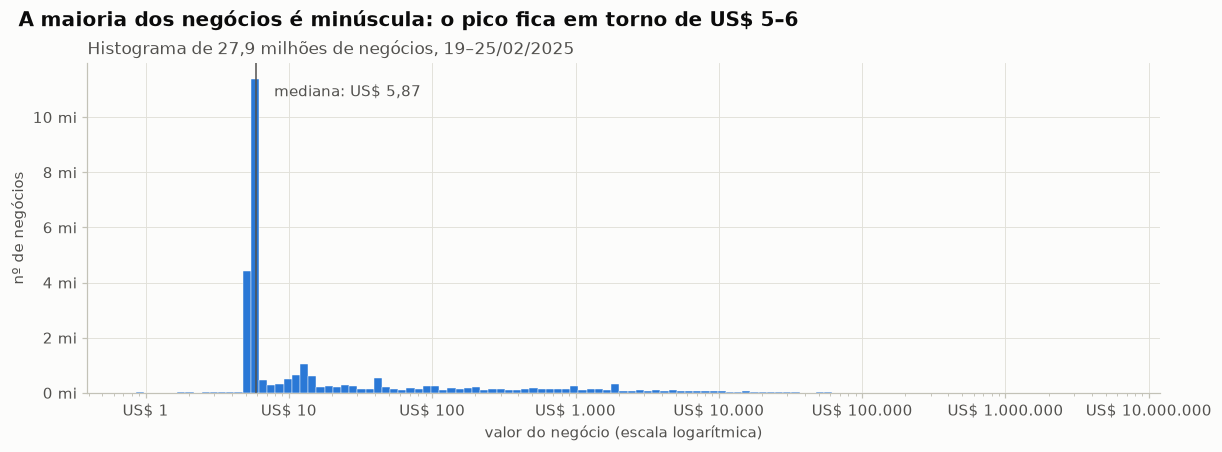
\includegraphics[width=\textwidth]{figuras/fig_hist_tamanho.png}
\end{center}
\fontedados
\end{figure}

\section{Concentração do volume por faixa de tamanho}\label{sec:faixas}

O agrupamento por faixa de tamanho (\code{groupby} em \code{size_bucket})
responde à segunda parte da pergunta P2: quem concentra o volume?

\begin{table}[htbp]
\caption{\label{tab:faixas}Negócios e volume financeiro por faixa de tamanho}
\begin{corpotabela}
\begin{tabularx}{\textwidth}{L{3.0cm}RRRRR}
\toprule
Faixa de tamanho & Negócios & Volume (\usd~mi) & Ticket mediano (\usd) & \% dos negócios & \% do volume \\
\midrule
$<$ \usd~100 & 23.123.213 & 276,70 & 5,78 & 82,80 & 1,50 \\
\usd~100 a 1 mil & 2.533.123 & 1.029,09 & 304,45 & 9,07 & 5,57 \\
\usd~1 mil a 10 mil & 1.871.733 & 6.118,64 & 2.134,25 & 6,70 & 33,14 \\
\usd~10 mil a 100 mil & 387.566 & 9.436,34 & 17.067,95 & 1,39 & 51,12 \\
$\geq$ \usd~100 mil & 9.703 & 1.599,66 & 120.057,53 & 0,03 & 8,67 \\
\midrule
Total & 27.925.338 & 18.460,44 & 5,87 & 100,00 & 100,00 \\
\bottomrule
\end{tabularx}
\end{corpotabela}
\fontedados
\end{table}

\begin{figure}[htbp]
\caption{\label{fig:faixas}Participação de cada faixa na contagem e no valor dos negócios}
\begin{center}
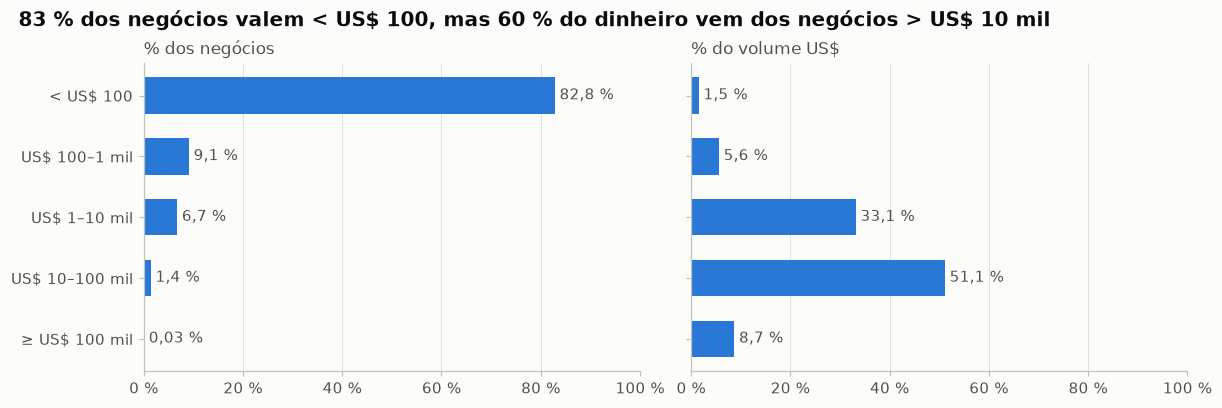
\includegraphics[width=\textwidth]{figuras/fig_faixas_tamanho.png}
\end{center}
\fontedados
\end{figure}

A \autoref{tab:faixas} e a \autoref{fig:faixas} mostram uma \textbf{concentração
extrema}: negócios abaixo de \usd~100 são 82,8\,\% da contagem e apenas 1,5\,\%
do valor, enquanto negócios a partir de \usd~10 mil são apenas 1,42\,\% da
contagem e respondem por 59,8\,\% do valor negociado. Para a mesa de execução,
contar negócios mede a atividade de robôs, e somar o valor financeiro mede a
liquidez de fato. As duas métricas contam histórias diferentes e precisam ser
vistas juntas.

\section{A semana em uma imagem}\label{sec:semana}

A \autoref{fig:precovolume} resume a semana: o preço subiu até o topo de
\usd~99.475 em 21/02, caiu com o ataque à Bybit, estabilizou no fim de semana e
desabou em 24 e 25/02, até o fundo de \usd~86.051. O volume por hora acompanha
os episódios de queda.

\begin{figure}[htbp]
\caption{\label{fig:precovolume}Preço de fechamento por minuto e volume por hora, de 19 a 25/02/2025}
\begin{center}
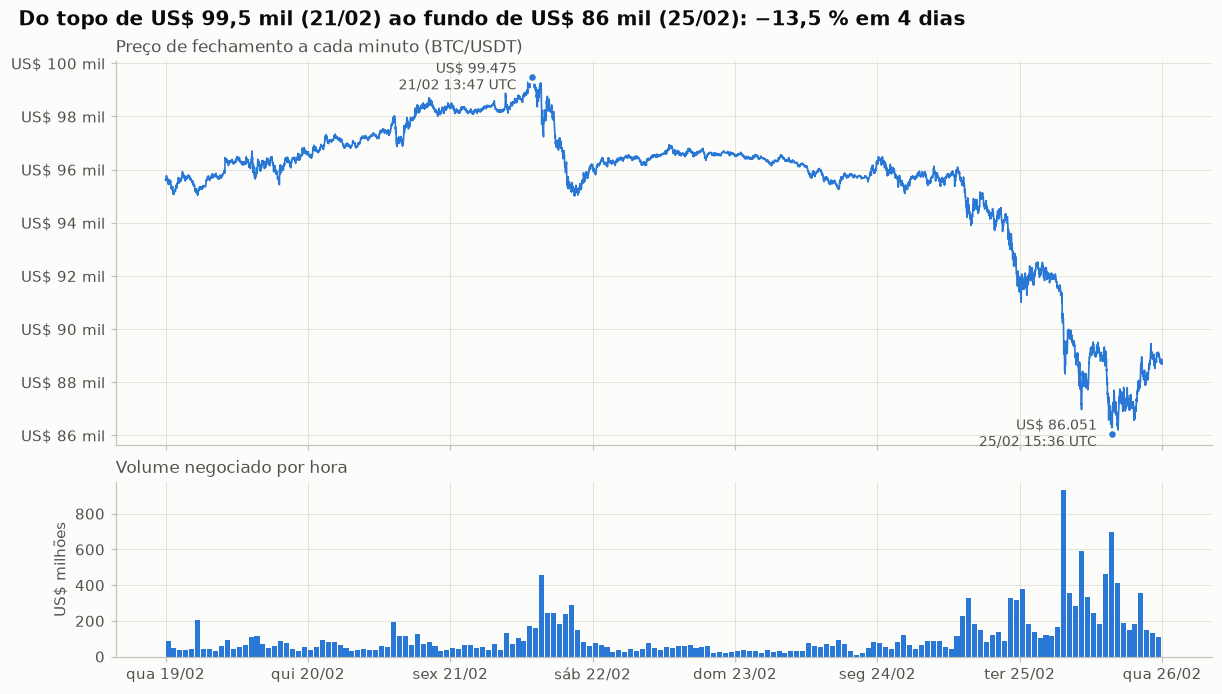
\includegraphics[width=\textwidth]{figuras/fig_preco_volume.png}
\end{center}
\fontedados
\end{figure}

\section{Resumo diário e dias de estresse}\label{sec:diario}

Para evitar a escolha subjetiva dos dias, cada dia foi classificado por uma
\textbf{regra objetiva}: amplitude intradiária
($\text{máxima}/\text{mínima} - 1$) acima de 4\,\% caracteriza um dia de
\textbf{estresse}; os demais são separados em dia útil e fim de semana, porque
no fim de semana o mercado é naturalmente mais calmo. A \autoref{tab:diario}
apresenta o resumo diário; a volatilidade realizada segue a
\autoref{eq:volrealizada}, e o saldo de fluxo é o OFI do dia em percentual.

\begin{table}[htbp]
\caption{\label{tab:diario}Resumo diário da semana e classificação dos dias}
\begin{corpotabela}
\setlength{\tabcolsep}{3.5pt}
\begin{tabular}{L{1.35cm}P{1.55cm}P{1.65cm}P{1.25cm}P{1.45cm}P{0.85cm}P{1.35cm}P{1.65cm}L{1.95cm}}
\toprule
Dia & Abertura & Fechamento & Retorno (\%) & Amplitude (\%) & VR (\%) & Volume (\usd~bi) & Negócios & Tipo \\
\midrule
qua 19/02 & 95.671,74 & 96.644,37 & 1,02 & 1,97 & 1,69 & 1,58 & 2.784.225 & dia útil \\
qui 20/02 & 96.644,37 & 98.305,00 & 1,72 & 2,38 & 1,48 & 1,66 & 2.386.973 & dia útil \\
sex 21/02 & 98.305,01 & 96.181,98 & $-2,16$ & 4,85 & 2,45 & 3,14 & 4.528.525 & estresse \\
sáb 22/02 & 96.181,99 & 96.551,01 & 0,38 & 1,26 & 0,97 & 1,09 & 1.506.418 & fim de semana \\
dom 23/02 & 96.551,01 & 96.258,00 & $-0,30$ & 1,49 & 0,93 & 1,04 & 1.457.368 & fim de semana \\
seg 24/02 & 96.258,00 & 91.552,88 & $-4,89$ & 5,64 & 2,56 & 2,98 & 4.972.684 & estresse \\
ter 25/02 & 91.552,88 & 88.680,40 & $-3,14$ & 7,54 & 4,72 & 6,96 & 10.289.145 & estresse \\
\bottomrule
\end{tabular}
\end{corpotabela}
\fonte{Elaborada pelos autores (2026), com dados de \citeonline{glitchlist2026}. VR: volatilidade realizada diária.}
\end{table}

\begin{figure}[htbp]
\caption{\label{fig:diario}Volume, número de negócios e volatilidade realizada por dia}
\begin{center}
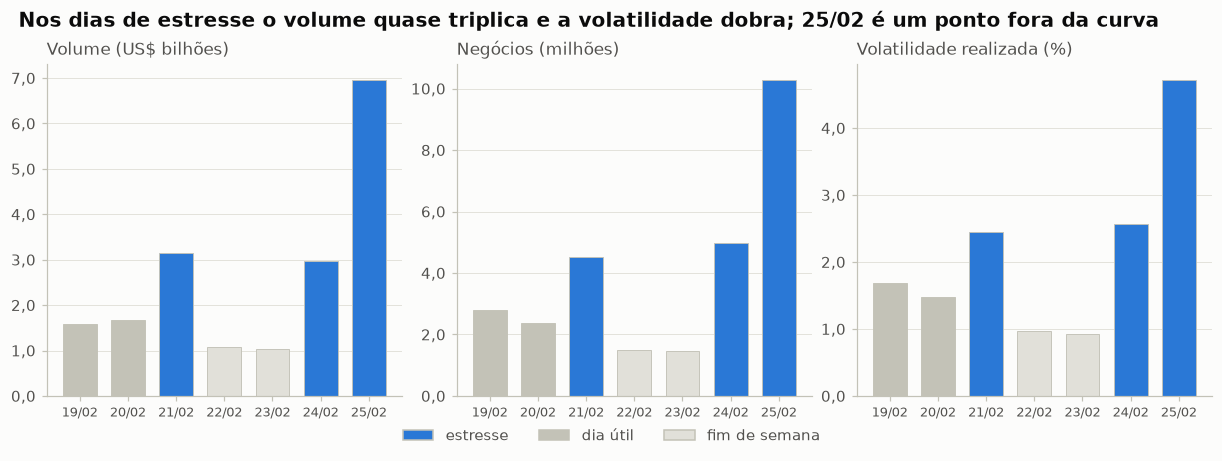
\includegraphics[width=\textwidth]{figuras/fig_resumo_diario.png}
\end{center}
\fontedados
\end{figure}

A \autoref{tab:regimes} compara as médias por tipo de dia. Nos dias de estresse
(21, 24 e 25/02), o volume foi \textbf{2,7 vezes} o de um dia útil normal, o
número de negócios 2,6 vezes e a volatilidade realizada \textbf{2,0 vezes}. O dia
25/02 é um ponto fora da curva: sozinho teve 10,3 milhões de negócios, cerca de
4 vezes um dia útil normal, e \usd~7 bilhões negociados
(\autoref{fig:diario}).

\begin{table}[htbp]
\caption{\label{tab:regimes}Médias diárias por tipo de dia e razão entre estresse e dia útil}
\begin{corpotabela}
\begin{tabular}{lrrrr}
\toprule
Tipo de dia & Volume (\usd~bi) & Negócios & VR (\%) & Amplitude (\%) \\
\midrule
Dia útil (19 e 20/02) & 1,62 & 2.585.599 & 1,59 & 2,17 \\
Fim de semana (22 e 23/02) & 1,07 & 1.481.893 & 0,95 & 1,38 \\
Estresse (21, 24 e 25/02) & 4,36 & 6.596.785 & 3,24 & 6,01 \\
\midrule
Razão estresse $\div$ dia útil & 2,69 & 2,55 & 2,04 & 2,76 \\
\bottomrule
\end{tabular}
\end{corpotabela}
\fontedados
\end{table}

O perfil de tamanho também muda. O agrupamento em dois níveis (tipo de dia
$\times$ faixa de tamanho) sobre as ordens agressoras mostra que, em estresse, as
ordens de \usd~100 mil ou mais passam de 35,9\,\% para 40,2\,\% do volume
(\autoref{tab:mixtamanho}). A \autoref{tab:grandes} mostra que só em 25/02
foram quase 10 mil dessas ordens, cerca de 4,5 vezes a média de um dia útil
normal, com ticket mediano estável perto de \usd~180 mil: o que cresce em
estresse é a quantidade de ordens institucionais, não o seu tamanho típico.

\begin{table}[htbp]
\caption{\label{tab:mixtamanho}Participação de cada faixa de tamanho no volume das ordens agressoras, por tipo de dia (\%)}
\begin{corpotabela}
\begin{tabular}{lrrrrr}
\toprule
Tipo de dia & $<$ \usd~100 & \usd~100 a 1 mil & \usd~1 a 10 mil & \usd~10 a 100 mil & $\geq$ \usd~100 mil \\
\midrule
Dia útil & 0,5 & 2,5 & 18,1 & 43,0 & 35,9 \\
Fim de semana & 0,6 & 3,6 & 17,2 & 40,8 & 37,9 \\
Estresse & 0,3 & 2,4 & 15,1 & 41,9 & 40,2 \\
\bottomrule
\end{tabular}
\end{corpotabela}
\fontedados
\end{table}

\begin{table}[htbp]
\caption{\label{tab:grandes}Ordens agressoras de \usd~100 mil ou mais, por dia}
\begin{corpotabela}
\begin{tabular}{lrrrr}
\toprule
Dia & Ordens & Volume (\usd~mi) & Ticket mediano (\usd~mil) & Maior ordem (\usd~mi) \\
\midrule
qua 19/02 & 2.066 & 531,8 & 177,8 & 3,1 \\
qui 20/02 & 2.346 & 631,6 & 187,6 & 5,1 \\
sex 21/02 & 5.100 & 1.367,0 & 185,0 & 3,4 \\
sáb 22/02 & 1.514 & 469,1 & 197,2 & 7,2 \\
dom 23/02 & 1.098 & 338,8 & 191,9 & 4,8 \\
seg 24/02 & 4.675 & 1.200,9 & 176,4 & 5,4 \\
ter 25/02 & 9.897 & 2.694,2 & 176,1 & 5,4 \\
\bottomrule
\end{tabular}
\end{corpotabela}
\fontedados
\end{table}

\section{Perfil intradiário da liquidez}\label{sec:intradiario}

Para a pergunta P1, usou-se a \textbf{mediana} por hora do dia: com apenas sete
dias, a média seria puxada pelos picos de 24 e 25/02. A
\autoref{fig:perfilhorario} mostra o volume, o número de negócios e a amplitude
medianos por minuto em cada hora UTC (no horário de Brasília, subtraem-se
3 horas).

\begin{figure}[htbp]
\caption{\label{fig:perfilhorario}Perfil horário de volume, negócios e amplitude por minuto (medianas, UTC)}
\begin{center}
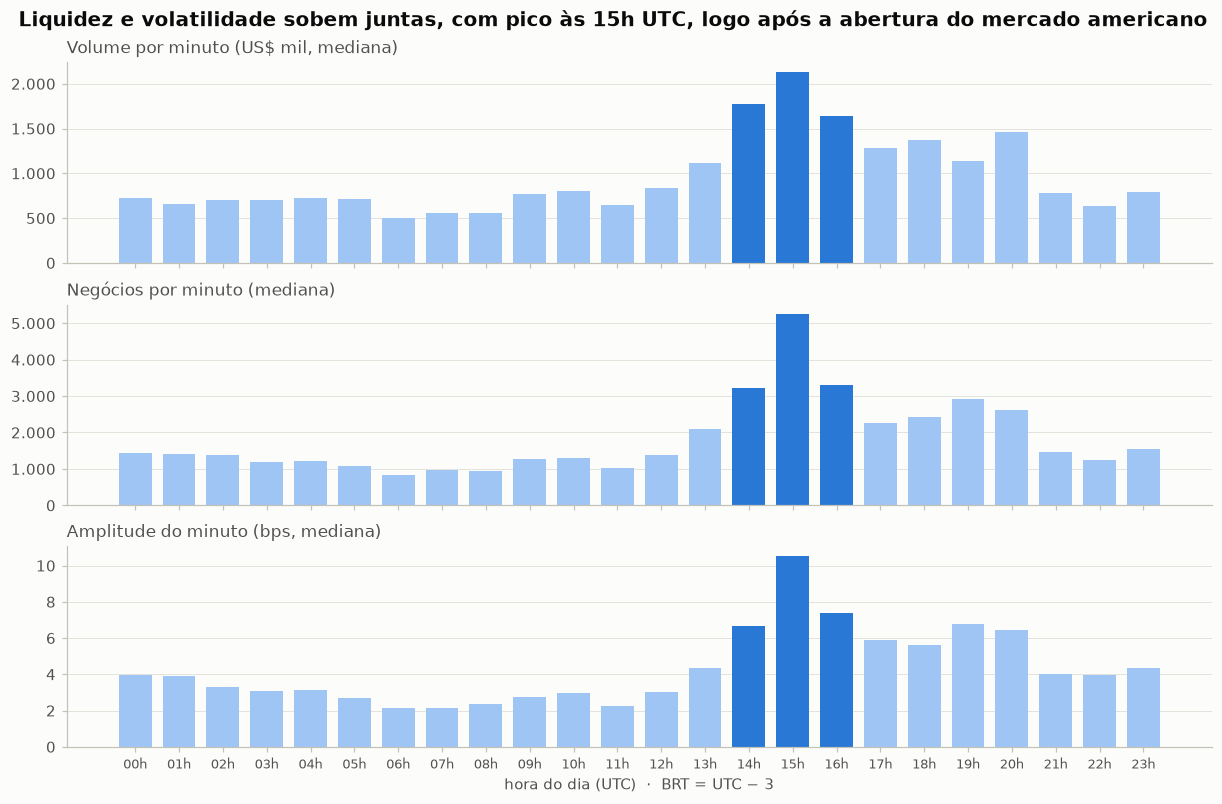
\includegraphics[width=\textwidth]{figuras/fig_perfil_horario.png}
\end{center}
\fontedados
\end{figure}

A liquidez é fortemente concentrada logo após a abertura do mercado americano,
entre 14h e 16h~UTC (11h e 13h em Brasília). Às 15h~UTC o volume mediano é de
\usd~2,13 milhões por minuto, \textbf{4,2 vezes} o das 06h~UTC (\usd~0,51 milhão
por minuto), a hora mais fraca. A volatilidade sobe junto: a correlação de
Spearman entre volume e amplitude é de $\rho = 0,83$ entre as 24 horas e de
$\rho = 0,79$ minuto a minuto. O mapa de calor da \autoref{fig:heatmap} revela,
porém, que a hora de maior volume da semana foi às 07h~UTC de 25/02, durante o
pânico: em estresse, a liquidez aparece fora do horário habitual.

\begin{figure}[htbp]
\caption{\label{fig:heatmap}Volume negociado por dia e hora (\usd~milhões por hora, UTC)}
\begin{center}
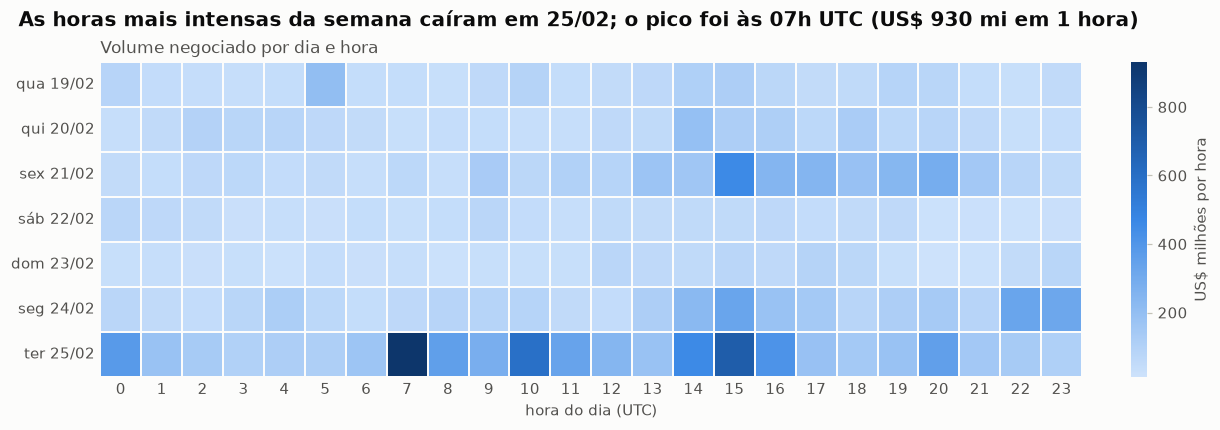
\includegraphics[width=\textwidth]{figuras/fig_heatmap_volume.png}
\end{center}
\fontedados
\end{figure}

\section{Retornos e caudas pesadas}\label{sec:caudas}

Os retornos de 1 minuto têm desvio-padrão $\sigma = 6,4$~bps e curtose em excesso
de 14,5. A \autoref{fig:caudas} compara o histograma observado, em escala
logarítmica, com uma distribuição normal de mesma média e desvio. Movimentos
além de $3\sigma$ ocorrem em \textbf{1,87\,\%} dos minutos, contra 0,27\,\% previstos
pela normal, ou seja, \textbf{6,9 vezes} mais, o que confirma as caudas pesadas
descritas por \citeonline{cont2001}. Para a mesa, limites de risco calibrados
pela curva normal subestimam a frequência de choques.

\begin{figure}[htbp]
\caption{\label{fig:caudas}Distribuição dos retornos de 1 minuto comparada à normal}
\begin{center}
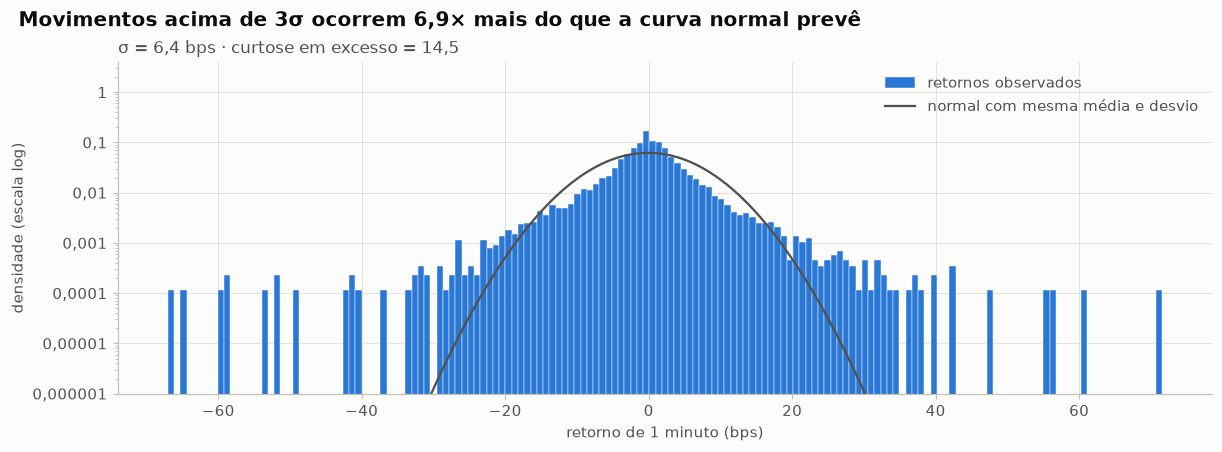
\includegraphics[width=\textwidth]{figuras/fig_caudas_retornos.png}
\end{center}
\fontedados
\end{figure}

\section{Pressão compradora e vendedora}\label{sec:pressao}

O saldo de fluxo agressor foi \textbf{negativo em todos os sete dias}, com mais
venda agressora que compra (de $-2,0\,\%$ em 20/02 a $-15,1\,\%$ em 23/02),
coerente com a queda de 13,5\,\% na semana. O painel direito da
\autoref{fig:ofi} mostra que, minuto a minuto, o OFI e o retorno do
\textbf{mesmo} minuto andam juntos.

\begin{figure}[htbp]
\caption{\label{fig:ofi}Saldo de fluxo diário e relação entre OFI e retorno no mesmo minuto}
\begin{center}
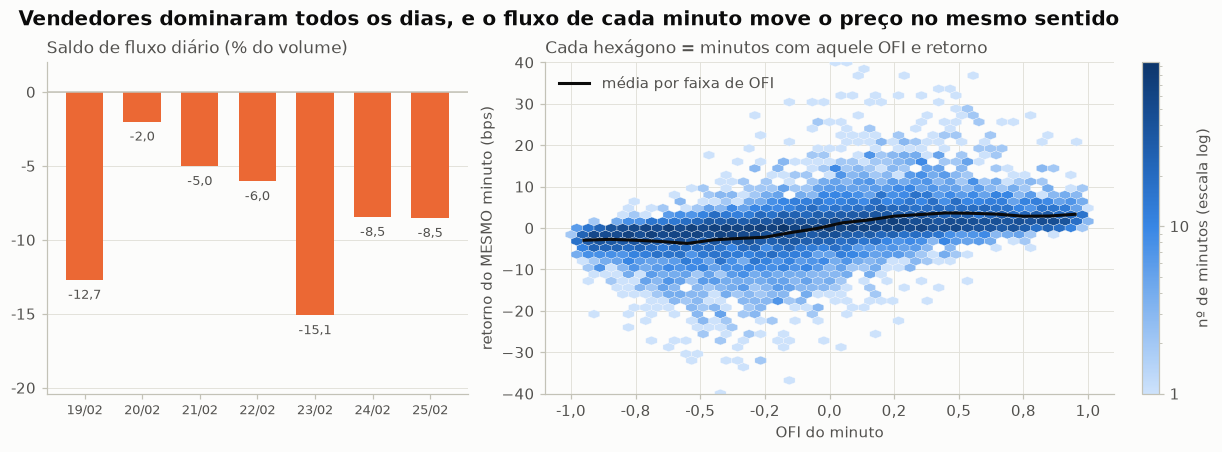
\includegraphics[width=\textwidth]{figuras/fig_ofi_fluxo.png}
\end{center}
\fontedados
\end{figure}

A pergunta P3, porém, é se o OFI \textbf{antecipa} o preço. A
\autoref{tab:defasagens} e a \autoref{fig:defasagens} mostram a correlação entre
o OFI do minuto $t$ e o retorno do minuto $t+k$. A faixa de ruído de 95\,\% para
$n = 10.080$ é $\pm 1,96/\sqrt{n} \approx \pm 0,0195$.

\begin{table}[htbp]
\caption{\label{tab:defasagens}Correlação entre $\mathrm{OFI}_t$ e $r_{t+k}$ para defasagens de 0 a 10 minutos}
\begin{corpotabela}
\setlength{\tabcolsep}{4.2pt}
\begin{tabular}{lrrrrrrrrrrr}
\toprule
$k$ (min) & 0 & 1 & 2 & 3 & 4 & 5 & 6 & 7 & 8 & 9 & 10 \\
\midrule
Pearson & 0,388 & 0,022 & 0,003 & $-0,017$ & $-0,008$ & $-0,016$ & $-0,010$ & $-0,005$ & $-0,007$ & 0,001 & $-0,010$ \\
Spearman & 0,545 & 0,038 & $-0,005$ & $-0,028$ & $-0,017$ & $-0,009$ & $-0,012$ & $-0,005$ & $-0,010$ & $-0,006$ & $-0,022$ \\
\bottomrule
\end{tabular}
\end{corpotabela}
\fontedados
\end{table}

\begin{figure}[htbp]
\caption{\label{fig:defasagens}Correlação de Pearson entre o OFI do minuto $t$ e o retorno do minuto $t+k$}
\begin{center}
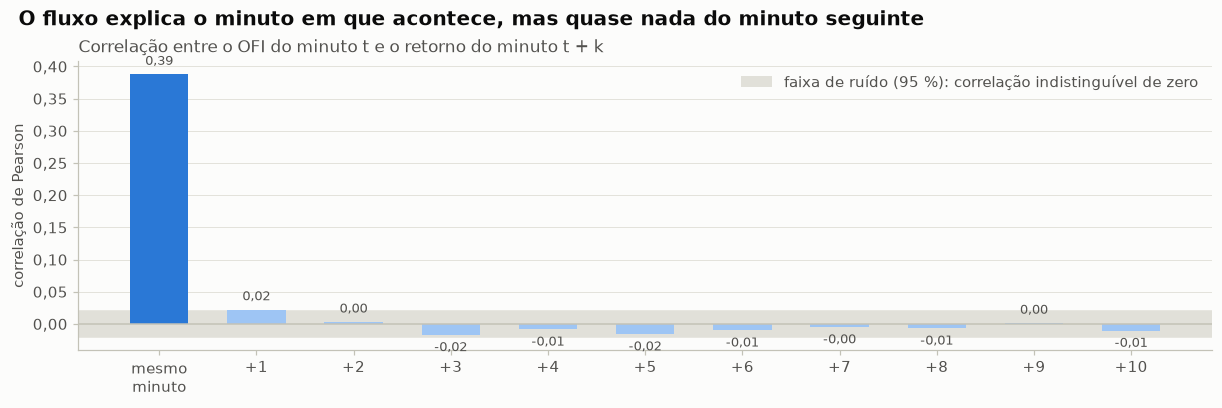
\includegraphics[width=\textwidth]{figuras/fig_ofi_defasagens.png}
\end{center}
\fontedados
\end{figure}

No mesmo minuto, a correlação de Pearson é de 0,388 (Spearman de 0,545): o fluxo
agressor empurra o preço no instante da execução. No minuto seguinte, cai para
0,022, pouco acima da faixa de ruído, o que explica apenas $r^2 \approx 0,05\,\%$
da variância do retorno, um valor economicamente desprezível. Da segunda
defasagem em diante, nenhum coeficiente de Pearson sai da faixa de ruído.

\section{Correlação entre as variáveis de 1 minuto}\label{sec:correlacao}

A \autoref{fig:spearman} mostra a matriz de correlação de Spearman, robusta às
caudas pesadas, entre as principais variáveis das barras de 1 minuto. Atividade
(volume e número de negócios), amplitude e retorno absoluto formam um bloco
fortemente correlacionado ($\rho$ entre 0,58 e 0,92). O OFI praticamente não se
relaciona com essas medidas de intensidade e só se liga ao retorno com sinal
($\rho = 0,55$). Essa separação antecipa o resultado do
\autoref{cap:modelagem}: a volatilidade é previsível a partir da atividade
recente, mas a direção não.

\begin{figure}[htbp]
\caption{\label{fig:spearman}Matriz de correlação de Spearman entre as variáveis de 1 minuto}
\begin{center}
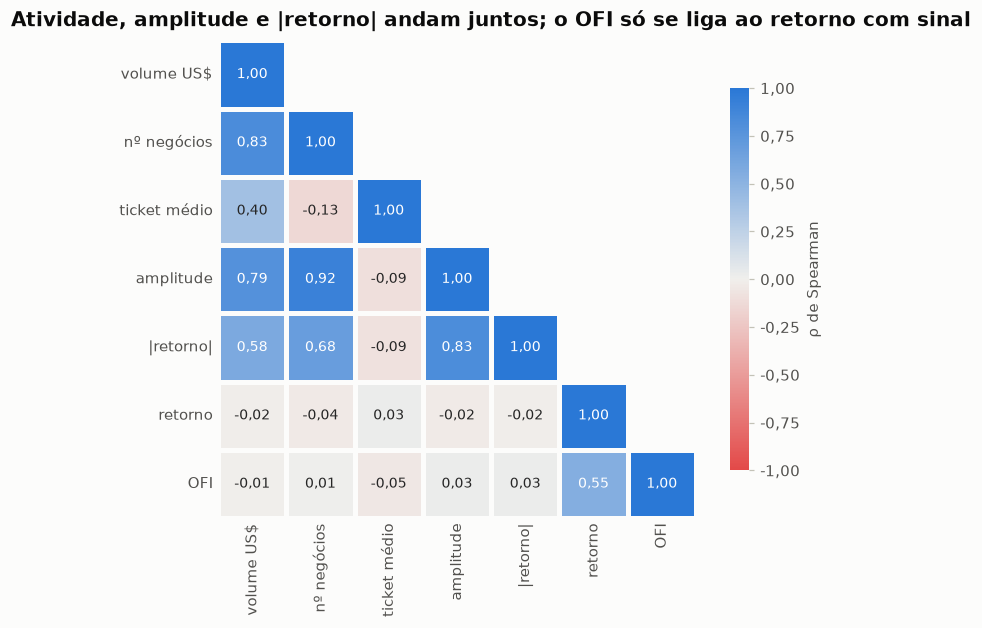
\includegraphics[width=0.78\textwidth]{figuras/fig_correlacao_spearman.png}
\end{center}
\fontedados
\end{figure}

\section{Respostas às perguntas de negócio}\label{sec:respostas}

A \autoref{tab:kpis} consolida os indicadores que respondem às três perguntas.

\begin{table}[htbp]
\caption{\label{tab:kpis}Indicadores-chave que respondem às perguntas P1 a P3}
\begin{corpotabela}
\begin{tabular}{llr}
\toprule
Pergunta & Indicador & Valor \\
\midrule
P1 & Hora de maior volume (mediana por minuto) & 15h UTC (\usd~2,13 mi/min) \\
P1 & Hora de menor volume (mediana por minuto) & 06h UTC (\usd~0,51 mi/min) \\
P1 & Razão entre pico e vale & 4,2 \\
P1 & Spearman entre volume e amplitude (24 horas) & 0,83 \\
P2 & Volume médio em estresse $\div$ dia útil & 2,7 \\
P2 & Volatilidade realizada em estresse $\div$ dia útil & 2,0 \\
P2 & Participação no volume dos negócios $\geq$ \usd~10 mil & 59,8\,\% \\
P2 & Participação na contagem dos negócios $\geq$ \usd~10 mil & 1,42\,\% \\
P3 & Correlação entre OFI e retorno no mesmo minuto & 0,388 \\
P3 & Correlação entre OFI e retorno do minuto seguinte & 0,022 \\
P3 & Dias com mais venda que compra agressora & 7 de 7 \\
\bottomrule
\end{tabular}
\end{corpotabela}
\fontedados
\end{table}

\textbf{P1 -- Liquidez e janela de execução.} A liquidez concentra-se entre 14h e
16h~UTC, com pico às 15h~UTC, e a volatilidade sobe junto. Para a mesa, isso é um
\textit{trade-off}: o horário mais líquido absorve ordens grandes com menos
impacto, mas expõe a execução a movimentos mais bruscos. A recomendação é fatiar
ordens grandes (TWAP ou VWAP) dentro da janela de liquidez, sem executar tudo de
uma vez nos minutos de pico de volatilidade, e monitorar deslocamentos da
liquidez em dias de choque.

\textbf{P2 -- Dias de estresse.} Pela regra objetiva, 21, 24 e 25/02 foram dias de
estresse, com volume 2,7 vezes e volatilidade 2,0 vezes maiores que um dia útil
normal. O volume é concentrado em poucos negócios grandes, e essa concentração
aumenta em estresse. Limites de risco e alertas devem ser calibrados pela
volatilidade realizada, e a infraestrutura deve suportar cerca de 4 vezes a carga
de um dia útil.

\textbf{P3 -- Fluxo de ordens.} O fluxo explica o retorno do minuto em que ocorre,
mas quase nada do minuto seguinte. De forma isolada e linear, o OFI de 1 minuto
não antecipa o preço de maneira útil, o que é consistente com um mercado
eficiente nessa escala \cite{fama1970}. O \autoref{cap:modelagem} testa essa
conclusão com horizontes mais curtos, combinações de variáveis e modelos não
lineares.

% =============================================================================
\chapter{Modelagem preditiva}\label{cap:modelagem}
% =============================================================================

Este capítulo documenta a etapa preditiva do \textit{Checkpoint}~3, implementada
em \code{src/modeling.py} e executada no notebook
\code{A3_CP3_modelagem_storytelling.ipynb}. A pergunta central é se informações
disponíveis no fechamento de um intervalo permitem antecipar algo útil sobre o
intervalo seguinte, sem que o modelo enxergue o futuro.

\section{Formulação dos problemas}\label{sec:formulacao}

Foram formulados dois problemas sobre o intervalo $t+1$, usando exclusivamente
informação disponível até o fechamento do intervalo $t$:

\begin{alineas}
  \item \textbf{tarefa A, volatilidade (regressão)}: prever a amplitude do
        intervalo seguinte e, como alvo alternativo, o retorno absoluto,
        \begin{equation}\label{eq:alvovol}
          y^{A}_t = \mathrm{amplitude}_{t+1}, \qquad
          y^{A'}_t = 10^4\,|r_{t+1}|;
        \end{equation}
  \item \textbf{tarefa B, direção (classificação binária)}: prever se o retorno
        do intervalo seguinte será positivo,
        \begin{equation}\label{eq:alvodir}
          y^{B}_t = \mathbb{I}\left(r_{t+1} > 0\right).
        \end{equation}
\end{alineas}

A tarefa A serve para calibrar limites dinâmicos de risco, o \textit{slippage}
esperado e o fatiamento TWAP ou VWAP. A tarefa B verifica se o desequilíbrio de
fluxo gera ganho direcional depois dos custos de transação. As duas tarefas
foram avaliadas em barras de 1 minuto (10.080) e de 1 segundo (604.800).

\section{Engenharia de atributos causais}\label{sec:atributos}

A função \code{build_lagged_features()} constrói os atributos a partir de cinco
defasagens, $\ell \in \{0, 1, 2, 3, 5\}$, em que $\ell = 0$ é o intervalo $t$
recém-fechado, e de três janelas móveis passadas, $w \in \{5, 15, 60\}$. Os
atributos se dividem em três famílias, combinadas em três conjuntos para um
estudo de ablação (\autoref{qua:atributos}). A lista completa dos 50 atributos
está no \autoref{apendice:atributos}.

\begin{quadro}[htbp]
\caption{\label{qua:atributos}Famílias e conjuntos de atributos dos modelos}
\begin{corpotabela}
\begin{tabularx}{\textwidth}{|L{2.6cm}|Y|C{1.9cm}|}
\hline
\textbf{Família} & \textbf{Atributos} & \textbf{Quantidade} \\ \hline
Fluxo (OFI) & $\mathrm{OFI}_{t-\ell}$ para cada defasagem; médias móveis do OFI em 5, 15 e 60 intervalos & 8 \\ \hline
Atividade & $\ln(1+\text{volume})$ e $\ln(1+\text{negócios})$ defasados; $\ln(1+\text{ticket médio})_t$; médias móveis de $\ln(1+\text{volume})$; interação $\mathrm{OFI}_t \times \ln(1+\text{volume}_t)$; nas barras de 1~s, também o indicador \code{has_trades} & 15 (16 em 1~s) \\ \hline
Volatilidade, retorno e sazonalidade & Amplitude, retorno absoluto e retorno defasados; médias móveis de amplitude e retorno absoluto e desvio-padrão móvel do retorno; razão de aceleração $\overline{\mathrm{amp}}_5 / (\overline{\mathrm{amp}}_{60} + 10^{-6})$; $\sin$ e $\cos$ da hora do dia & 27 \\ \hline
\multicolumn{3}{|l|}{\textbf{Conjuntos de ablação}: \code{apenas_ofi} (8 atributos) $\subset$ \code{fluxo_e_atividade} (23) $\subset$ \code{completo} (50; 51 em 1~s)} \\ \hline
\end{tabularx}
\end{corpotabela}
\fonteautores[Elaborado]
\end{quadro}

A sazonalidade intradiária entra por codificação cíclica, que é determinística e
portanto conhecida com antecedência, com $h_t$ igual à hora do dia em fração
(por exemplo, 14,5 para 14h30):

\begin{equation}\label{eq:sazonal}
  s_t = \sin\!\left(\frac{2\pi h_t}{24}\right), \qquad
  c_t = \cos\!\left(\frac{2\pi h_t}{24}\right).
\end{equation}

\section{Prevenção do vazamento de informação futura}\label{sec:vazamento}

Em microestrutura de alta frequência, qualquer erro sutil cria uma acurácia
artificial que desaparece em produção. O pipeline adota quatro salvaguardas:

\begin{alineas}
  \item os atributos usam apenas defasagens positivas (\code{shift(k)} com
        $k \geq 0$) e janelas móveis que terminam em $t$; nenhuma operação usa
        \code{shift(-k)} ou janelas centradas; apenas os alvos olham para
        $t+1$;
  \item as lacunas das barras de 1 segundo são preenchidas pelo último valor
        conhecido, nunca por interpolação (\autoref{sec:gaps});
  \item a padronização (\code{StandardScaler}) faz parte de um \code{Pipeline} e
        é ajustada apenas na dobra de treino;
  \item um teste de perturbação comprova a causalidade: alterar drasticamente
        todas as barras a partir de um instante (multiplicar preços, fixar o OFI
        em $-1$) não pode mudar nenhum atributo anterior a esse instante. O
        teste é executado no notebook e no conjunto de testes automatizados.
\end{alineas}

Após remover apenas as bordas incompletas (as primeiras 60 barras, exigidas pela
maior janela, e a última, que não tem alvo), restaram \textbf{10.019
observações} em 1 minuto e \textbf{604.739} em 1 segundo.

\section{Validação \textit{walk-forward}}\label{sec:validacaowf}

A validação usa dobras diárias com janela de treino expansiva
(\autoref{fig:walkforward}). Para cada dia de teste $d_k$, o conjunto de treino é
$\mathcal{T}_k = \{t : \mathrm{dia}(t) < d_k\}$ e o de teste é
$\mathcal{V}_k = \{t : \mathrm{dia}(t) = d_k\}$. Com mínimo de dois dias de
treino, há cinco dobras, que testam estritamente fora da amostra os dias 21 a
25/02 e cobrem tanto dias calmos quanto dias de estresse. As métricas são
calculadas em cada dobra e resumidas pela média simples entre as cinco.

\begin{figure}[htbp]
\caption{\label{fig:walkforward}Esquema das dobras de validação \textit{walk-forward} diária}
\begin{center}
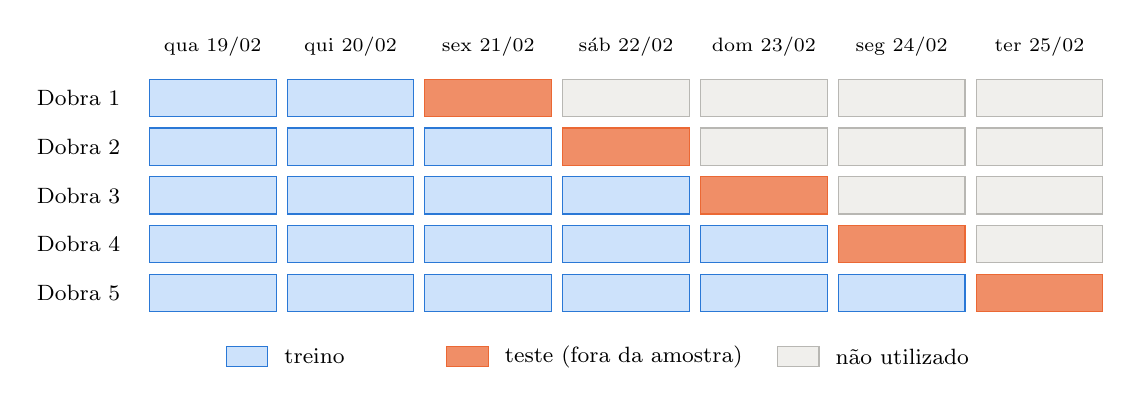
\begin{tikzpicture}[font=\footnotesize, x=1.75cm, y=0.62cm]
  \foreach \d [count=\i from 0] in {qua 19/02, qui 20/02, sex 21/02, sáb 22/02, dom 23/02, seg 24/02, ter 25/02}{
    \node[anchor=south, font=\scriptsize] at (\i+0.5, 0.15) {\d};
  }
  \foreach \k in {1,...,5}{
    \pgfmathtruncatemacro{\teste}{\k+1}
    \node[anchor=east] at (-0.1, -\k+0.5) {Dobra \k};
    \foreach \j in {0,...,6}{
      \ifnum\j<\teste
        \fill[azulclaro, draw=azul, line width=0.4pt] (\j+0.04,-\k+0.12) rectangle (\j+0.96,-\k+0.88);
      \else\ifnum\j=\teste
        \fill[laranja!75, draw=laranja, line width=0.4pt] (\j+0.04,-\k+0.12) rectangle (\j+0.96,-\k+0.88);
      \else
        \fill[cinzaclaro, draw=cinza!60, line width=0.4pt] (\j+0.04,-\k+0.12) rectangle (\j+0.96,-\k+0.88);
      \fi\fi
    }
  }
  \fill[azulclaro, draw=azul] (0.6,-6.0) rectangle (0.9,-5.6);
  \node[anchor=west] at (0.95,-5.8) {treino};
  \fill[laranja!75, draw=laranja] (2.2,-6.0) rectangle (2.5,-5.6);
  \node[anchor=west] at (2.55,-5.8) {teste (fora da amostra)};
  \fill[cinzaclaro, draw=cinza!60] (4.6,-6.0) rectangle (4.9,-5.6);
  \node[anchor=west] at (4.95,-5.8) {não utilizado};
\end{tikzpicture}
\end{center}
\fonteautores
\end{figure}

\section{Modelos e métricas}\label{sec:modelos}

Cada tarefa compara dois \textit{baselines} ingênuos, um modelo linear e um
modelo não linear baseado em árvores (\autoref{qua:modelos}). Os
\textit{baselines} são essenciais: um modelo só tem valor se superar regras
simples que qualquer operador aplicaria sem estatística.

\begin{quadro}[htbp]
\caption{\label{qua:modelos}Modelos avaliados e seus hiperparâmetros}
\begin{corpotabela}
\begin{tabularx}{\textwidth}{|L{1.4cm}|L{4.3cm}|L{2.4cm}|Y|}
\hline
\textbf{Tarefa} & \textbf{Modelo} & \textbf{Atributos} & \textbf{Especificação} \\ \hline
\multirow{6}{=}{A (regressão)}
 & Persistência & -- & Prevê a amplitude (ou retorno absoluto) de $t+1$ igual à de $t$ \\ \cline{2-4}
 & Média móvel (15) & -- & Prevê a média dos últimos 15 intervalos \\ \cline{2-4}
 & Ridge & \code{apenas_ofi}; \code{completo} & Padronização e regressão linear com penalidade L2, $\alpha = 10$ \\ \cline{2-4}
 & \textit{HistGradientBoosting} & \code{fluxo_e_atividade}; \code{completo} & 150 iterações, profundidade 5, taxa 0,05, mínimo de 50 amostras por folha, semente 42 \\ \hline
\multirow{6}{=}{B (classifi\-cação)}
 & Classe majoritária & -- & Probabilidade constante igual à frequência de alta no treino \\ \cline{2-4}
 & Persistência de sinal & -- & Prevê alta se o retorno de $t$ foi positivo (probabilidade 0,99 ou 0,01) \\ \cline{2-4}
 & Regressão logística & \code{apenas_ofi}; \code{completo} & Padronização e penalidade L2 com $C = 0,5$, até 500 iterações \\ \cline{2-4}
 & \textit{HistGradientBoosting} & \code{fluxo_e_atividade}; \code{completo} & Mesmos hiperparâmetros da tarefa A \\ \hline
\end{tabularx}
\end{corpotabela}
\fonteautores[Elaborado]
\end{quadro}

Na tarefa A, as previsões negativas são truncadas em zero. As métricas de
regressão são o erro absoluto médio (MAE), a raiz do erro quadrático médio
(RMSE), o coeficiente de determinação fora da amostra e a correlação de postos
de Spearman entre previsto e realizado:

\begin{equation}\label{eq:metricasreg}
  \mathrm{MAE} = \frac{1}{n}\sum_{t}|y_t - \hat{y}_t|, \qquad
  \mathrm{RMSE} = \sqrt{\frac{1}{n}\sum_{t}(y_t - \hat{y}_t)^2}, \qquad
  R^2 = 1 - \frac{\sum_t (y_t - \hat{y}_t)^2}{\sum_t (y_t - \bar{y})^2}.
\end{equation}

\noindent Fora da amostra, $R^2$ pode ser negativo, o que indica um modelo pior
que prever a média do próprio dia de teste. Na tarefa B, além de acurácia,
acurácia balanceada, ROC-AUC e perda logarítmica, mede-se o \textbf{retorno
bruto} de uma estratégia que compra quando $\hat{p}_t \geq 0,5$ e vende caso
contrário,

\begin{equation}\label{eq:retornobruto}
  \bar{g} = \frac{1}{n}\sum_{t} s_t \cdot 10^4\, r_{t+1}, \qquad
  s_t = \begin{cases} +1, & \hat{p}_t \geq 0,5,\\ -1, & \hat{p}_t < 0,5, \end{cases}
\end{equation}

\noindent e o mesmo retorno restrito aos 10\,\% de sinais mais confiantes, isto
é, aos intervalos em que $|\hat{p}_t - 0,5|$ está acima do seu percentil 90. O
retorno bruto não desconta taxas; ele é comparado depois aos custos de execução.

\section{Resultados em barras de 1 minuto}\label{sec:resultados1m}

\subsection{Volatilidade}\label{sec:vol1m}

\begin{table}[htbp]
\caption{\label{tab:vol1m}Previsão da amplitude do minuto seguinte: médias das cinco dobras}
\begin{corpotabela}
\begin{tabular}{llrrrr}
\toprule
Modelo & Família & MAE (bps) & RMSE (bps) & $R^2$ & Spearman \\
\midrule
Persistência & \textit{baseline} & 3,296 & 4,871 & 0,074 & 0,530 \\
Média móvel (15) & \textit{baseline} & 2,775 & 4,154 & 0,353 & 0,603 \\
Ridge (apenas OFI) & linear & 5,297 & 7,265 & $-0,963$ & 0,044 \\
\textbf{Ridge (completo)} & linear & \textbf{2,668} & \textbf{3,999} & \textbf{0,385} & \textbf{0,616} \\
HGB (fluxo e atividade) & não linear & 2,924 & 4,414 & 0,301 & 0,583 \\
HGB (completo) & não linear & 2,835 & 4,320 & 0,314 & 0,574 \\
\bottomrule
\end{tabular}
\end{corpotabela}
\fonte{Elaborada pelos autores (2026), com dados de \citeonline{glitchlist2026}. HGB: \textit{HistGradientBoosting}.}
\end{table}

A \autoref{tab:vol1m} mostra que a volatilidade do minuto seguinte é previsível.
O Ridge com todos os atributos teve o melhor desempenho em todas as métricas
($R^2 = 0,385$, Spearman de 0,616), superando a média móvel de 15 minutos, que
já é um \textit{baseline} forte ($R^2 = 0,353$). O OFI sozinho não prevê
volatilidade ($R^2 < 0$), o que é coerente com a matriz de correlação da
\autoref{fig:spearman}. Os modelos de árvore ficaram atrás do Ridge porque não
extrapolam: suas previsões ficam limitadas aos valores vistos no treino, e o
pânico de 25/02 produziu amplitudes acima de tudo o que havia nos dias
anteriores. O painel direito da \autoref{fig:modvol} ilustra esse efeito.

\begin{figure}[htbp]
\caption{\label{fig:modvol}Desempenho na previsão de volatilidade e série prevista em 25/02}
\begin{center}
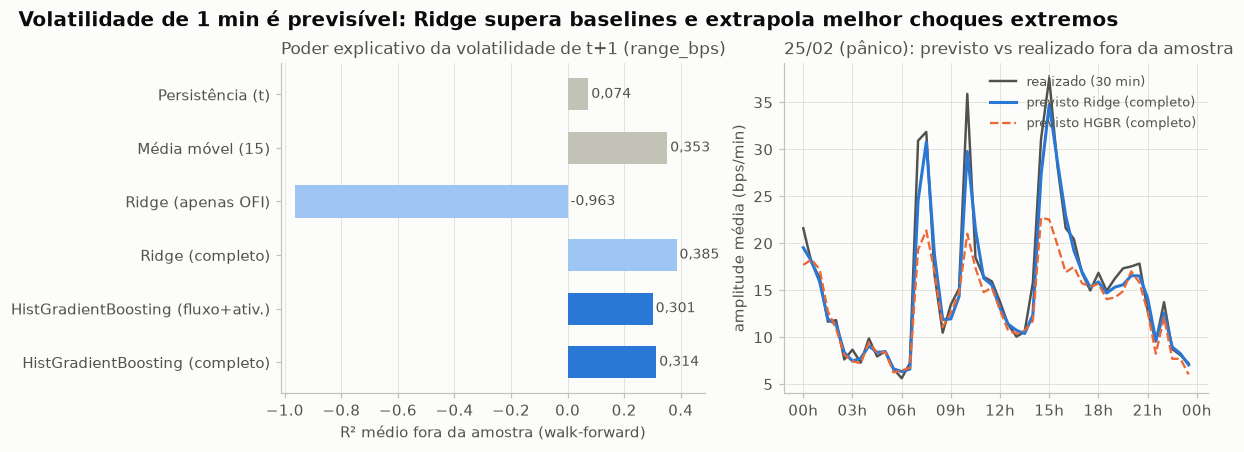
\includegraphics[width=\textwidth]{figuras/fig_modelo_volatilidade.png}
\end{center}
\fontedados
\end{figure}

Com o alvo alternativo, o retorno absoluto do minuto seguinte, o padrão se repete
em nível mais baixo, porque o retorno absoluto é uma medida mais ruidosa que a
amplitude: Ridge (completo) obteve $R^2 = 0,154$ e Spearman de 0,370, contra
$R^2 = 0,146$ da média móvel e $R^2 = -0,482$ da persistência.

\subsection{Direção do retorno}\label{sec:dir1m}

\begin{table}[htbp]
\caption{\label{tab:dir1m}Previsão da direção do minuto seguinte: médias das cinco dobras}
\begin{corpotabela}
\setlength{\tabcolsep}{4pt}
\begin{tabularx}{\textwidth}{L{3.6cm}RRRRRR}
\toprule
Modelo & Acurácia & Acur. balanc. & ROC-AUC & Perda log. & Ret. bruto (bps) & Ret. top 10\,\% (bps) \\
\midrule
Classe majoritária & 0,510 & 0,500 & 0,500 & 0,693 & 0,091 & 0,091 \\
Persistência de sinal & 0,530 & 0,529 & 0,529 & 2,172 & 0,257 & 0,257 \\
\textbf{Logit (apenas OFI)} & 0,526 & 0,524 & \textbf{0,536} & \textbf{0,691} & 0,155 & \textbf{0,360} \\
Logit (completo) & 0,517 & 0,516 & 0,523 & 0,699 & $-0,004$ & $-0,178$ \\
HGB (fluxo e atividade) & 0,520 & 0,520 & 0,521 & 0,705 & 0,172 & 0,330 \\
HGB (completo) & 0,511 & 0,511 & 0,513 & 0,709 & 0,015 & $-0,119$ \\
\bottomrule
\end{tabularx}
\end{corpotabela}
\fonte{Elaborada pelos autores (2026), com dados de \citeonline{glitchlist2026}. A perda logarítmica alta da persistência decorre das probabilidades extremas (0,01 e 0,99).}
\end{table}

A direção do minuto seguinte fica próxima do acaso (\autoref{tab:dir1m}). O
melhor ROC-AUC, de 0,536, é da regressão logística apenas com OFI, e o melhor
retorno bruto nos 10\,\% de sinais mais confiantes é de $+0,36$~bps por operação.
Acrescentar atributos piorou o resultado fora da amostra, sinal de que os modelos
mais ricos aprendem ruído. A \autoref{fig:moddir} compara esses ganhos com os
custos de execução.

\begin{figure}[htbp]
\caption{\label{fig:moddir}Discriminação direcional e retorno bruto contra o custo de transação}
\begin{center}
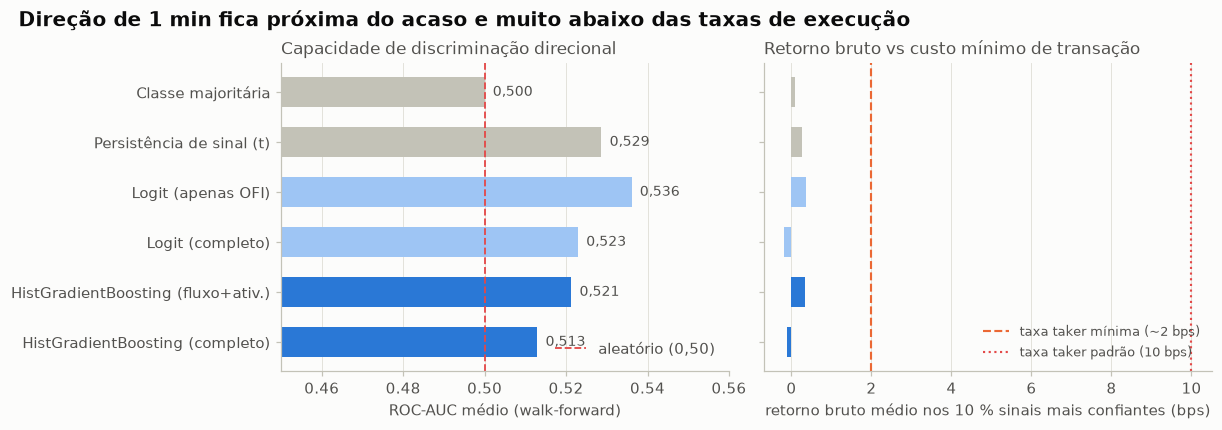
\includegraphics[width=\textwidth]{figuras/fig_modelo_direcao.png}
\end{center}
\fontedados
\end{figure}

\section{Resultados em barras de 1 segundo}\label{sec:resultados1s}

No \textit{Checkpoint}~2, levantou-se a hipótese de que o poder preditivo do
fluxo pudesse aparecer em escalas menores que 1 minuto. O mesmo pipeline causal
e \textit{walk-forward} foi aplicado às 604.800 barras de 1 segundo. Na
classificação, foram avaliados apenas os segundos em que o preço variou
($r_{t+1} \neq 0$), para evitar que segundos ``planos'' inflassem a acurácia.

\begin{table}[htbp]
\caption{\label{tab:vol1s}Previsão da amplitude do segundo seguinte: médias das cinco dobras}
\begin{corpotabela}
\begin{tabular}{llrrrr}
\toprule
Modelo & Família & MAE (bps) & RMSE (bps) & $R^2$ & Spearman \\
\midrule
Persistência & \textit{baseline} & 0,341 & 0,719 & $-0,465$ & 0,352 \\
Média móvel (15) & \textit{baseline} & 0,306 & 0,556 & 0,121 & 0,380 \\
Ridge (apenas OFI) & linear & 0,369 & 0,666 & $-0,149$ & 0,100 \\
\textbf{Ridge (completo)} & linear & \textbf{0,302} & \textbf{0,543} & \textbf{0,164} & 0,427 \\
HGB (fluxo e atividade) & não linear & 0,312 & 0,560 & 0,126 & \textbf{0,434} \\
HGB (completo) & não linear & 0,306 & 0,550 & 0,150 & 0,430 \\
\bottomrule
\end{tabular}
\end{corpotabela}
\fontedados
\end{table}

\begin{table}[htbp]
\caption{\label{tab:dir1s}Previsão da direção do segundo seguinte, apenas segundos com variação de preço}
\begin{corpotabela}
\setlength{\tabcolsep}{4pt}
\begin{tabularx}{\textwidth}{L{3.6cm}RRRRRR}
\toprule
Modelo & Acurácia & Acur. balanc. & ROC-AUC & Perda log. & Ret. bruto (bps) & Ret. top 10\,\% (bps) \\
\midrule
Classe majoritária & 0,503 & 0,500 & 0,500 & 0,693 & $-0,004$ & $-0,004$ \\
Persistência de sinal & 0,456 & 0,457 & 0,457 & 2,511 & 0,117 & 0,117 \\
Logit (apenas OFI) & 0,549 & 0,549 & 0,582 & 0,685 & $-0,096$ & $-0,106$ \\
Logit (completo) & 0,635 & 0,635 & 0,695 & 0,633 & 0,082 & 0,135 \\
HGB (fluxo e atividade) & 0,676 & 0,676 & 0,754 & 0,573 & 0,105 & 0,061 \\
\textbf{HGB (completo)} & \textbf{0,781} & \textbf{0,781} & \textbf{0,837} & \textbf{0,470} & 0,106 & 0,054 \\
\bottomrule
\end{tabularx}
\end{corpotabela}
\fontedados
\end{table}

Em volatilidade (\autoref{tab:vol1s}), os modelos com todos os atributos voltam a
superar os \textit{baselines}, com Spearman em torno de 0,43 contra 0,35 da
persistência. Em direção (\autoref{tab:dir1s}), o resultado parece
surpreendente: o \textit{HistGradientBoosting} com todos os atributos acerta
78,1\,\% das direções, com ROC-AUC de 0,837. A explicação está na própria tabela:
a persistência de sinal acerta só 45,6\,\%, ou seja, em 54,4\,\% dos casos o
segundo seguinte \textbf{reverte} o anterior. É o \textit{bid-ask bounce}
descrito por \citeonline{roll1984}: o último preço oscila entre a melhor
oferta de compra e a de venda conforme o lado do agressor, e o modelo aprende a
prever esse rebote de um \textit{tick}. Como o movimento previsto é minúsculo, o
retorno bruto médio é de apenas $+0,11$~bps por operação ($+0,05$~bps nos sinais
mais confiantes).

\section{Viabilidade operacional}\label{sec:viabilidade}

A taxa \textit{taker} da Binance no mercado à vista varia, conforme o nível do
cliente, de cerca de 2 a 10~bps por perna \cite{binancefees}; uma operação
completa paga duas pernas, além do \textit{slippage}. O \autoref{qua:viabilidade}
confronta os resultados com esses custos.

\begin{quadro}[htbp]
\caption{\label{qua:viabilidade}Viabilidade operacional dos sinais para a mesa de execução}
\begin{corpotabela}
\begin{tabularx}{\textwidth}{|L{2.6cm}|Y|L{4.4cm}|}
\hline
\textbf{Dimensão} & \textbf{Evidência em 1 minuto e 1 segundo} & \textbf{Veredito} \\ \hline
Previsão de volatilidade & Em 1~min, Ridge (completo) atinge $R^2 = 0,385$ e Spearman de 0,616, acima da média móvel de 15 minutos ($R^2 = 0,353$) e dos modelos de árvore. Em 1~s, Ridge e HGB atingem Spearman de cerca de 0,43. O OFI sozinho não prevê volatilidade. & \textbf{Viável e recomendada}: usar a previsão do Ridge para calibrar limites dinâmicos de \textit{slippage}, alertas e o ritmo do fatiamento TWAP ou VWAP. \\ \hline
Previsão de direção & Em 1~min, o melhor ROC-AUC é de 0,536, com retorno bruto de $+0,36$~bps nos sinais mais confiantes. Em 1~s, a acurácia de 78,1\,\% captura o \textit{bid-ask bounce}, com retorno bruto de $+0,11$~bps. & \textbf{Inviável para operar direção}: o ganho bruto, abaixo de 0,4~bps, é muito menor que o custo de 2 a 10~bps por perna. Útil apenas como filtro passivo de \textit{timing}. \\ \hline
\end{tabularx}
\end{corpotabela}
\fonteautores[Elaborado]
\end{quadro}

O resultado confirma a hipótese formulada para a pergunta P3: o fluxo agressor
explica o preço no instante em que ocorre, mas não gera previsão direcional
lucrativa, o que é consistente com a eficiência de mercado nessa escala
\cite{fama1970}. Por outro lado, a volatilidade tem persistência e sazonalidade
suficientes para ser prevista, e é essa previsão que tem valor prático imediato
para a mesa.

% =============================================================================
\chapter{Painel interativo}\label{cap:dashboard}
% =============================================================================

O painel interativo, implementado em \code{app/dashboard.py} com Streamlit
\cite{streamlit2026} e Plotly \cite{plotly2015}, é o produto de visualização do
\textit{Checkpoint}~3. Ele permite que a mesa de execução explore os indicadores
das perguntas P1 a P3 com filtros por dia, janela horária, fuso e faixa de
tamanho, e consulte os resultados da modelagem.

\section{Arquitetura e desempenho}\label{sec:dasharquitetura}

O painel não acessa a base bruta: ele consome somente os Parquets de
\code{data/processed/}, por meio das funções de \code{src/data_loader.py} e
\code{src/modeling.py}. Se os arquivos não existirem, exibe uma mensagem pedindo
que o ETL seja executado antes. Para manter a interação fluida, as operações
custosas são memorizadas com o decorador \code{st.cache_data} e executadas uma
única vez por sessão do servidor:

\begin{alineas}
  \item leitura das barras de 1 minuto;
  \item resumos centrais: resumo diário, distribuição de negócios por dia, hora e
        faixa de tamanho (com \textit{cache} adicional em
        \code{trade_size_hourly.parquet}) e agregação das ordens agressoras por
        dia, hora e faixa, incluindo a contagem e o volume das ordens de
        \usd~100 mil ou mais;
  \item validação \textit{walk-forward} completa em barras de 1 minuto, para as
        tarefas de volatilidade e direção.
\end{alineas}

Os filtros são aplicados depois, sobre esses resumos já agregados, o que evita
reprocessar os 27,9 milhões de negócios a cada clique.

\section{Filtros}\label{sec:filtros}

\begin{quadro}[htbp]
\caption{\label{qua:filtros}Filtros da barra lateral do painel}
\begin{corpotabela}
\begin{tabularx}{\textwidth}{|L{3.4cm}|L{4.2cm}|Y|}
\hline
\textbf{Filtro} & \textbf{Opções} & \textbf{Efeito} \\ \hline
Fuso horário & UTC; BRT (UTC$-3$) & Desloca o eixo horário de todos os perfis, barras e mapas de calor \\ \hline
Recorte rápido de dias & Semana completa; apenas dias de estresse (21, 24 e 25/02); apenas dias calmos (19, 20, 22 e 23/02); seleção manual & Pré-seleciona os dias do filtro seguinte \\ \hline
Dias incluídos & Cada dia, rotulado com o tipo (por exemplo, ``ter 25/02 $\cdot$ estresse'') & Restringe todos os gráficos e indicadores aos dias escolhidos \\ \hline
Janela horária & Intervalo de 0h a 23h no fuso escolhido & Restringe barras, perfis e agregações às horas escolhidas \\ \hline
Faixas de tamanho & As cinco faixas de \code{size_bucket} & Restringe as análises de concentração por tamanho (P2) \\ \hline
\end{tabularx}
\end{corpotabela}
\fonteautores[Elaborado]
\end{quadro}

Duas decisões de projeto devem ser conhecidas por quem usa o painel. Primeiro, o
filtro de dias usa a data em UTC; ao escolher BRT, muda o rótulo das horas, mas
cada dia continua delimitado pela meia-noite UTC. Segundo, as tabelas de
modelagem da aba P3 resumem a validação \textit{walk-forward} da semana inteira e
não respondem aos filtros, porque o treino depende da sequência completa de dias.

\section{Indicadores e abas}\label{sec:abas}

O topo do painel exibe o título, um resumo do filtro ativo e cinco indicadores
recalculados a cada mudança de filtro. Abaixo deles, quatro abas organizam o
conteúdo segundo a narrativa do projeto. A \autoref{fig:wireframe} mostra um
esquema da interface, e o \autoref{qua:abas} detalha o conteúdo de cada aba.

\begin{figure}[htbp]
\caption{\label{fig:wireframe}Esquema da interface do painel interativo}
\begin{center}
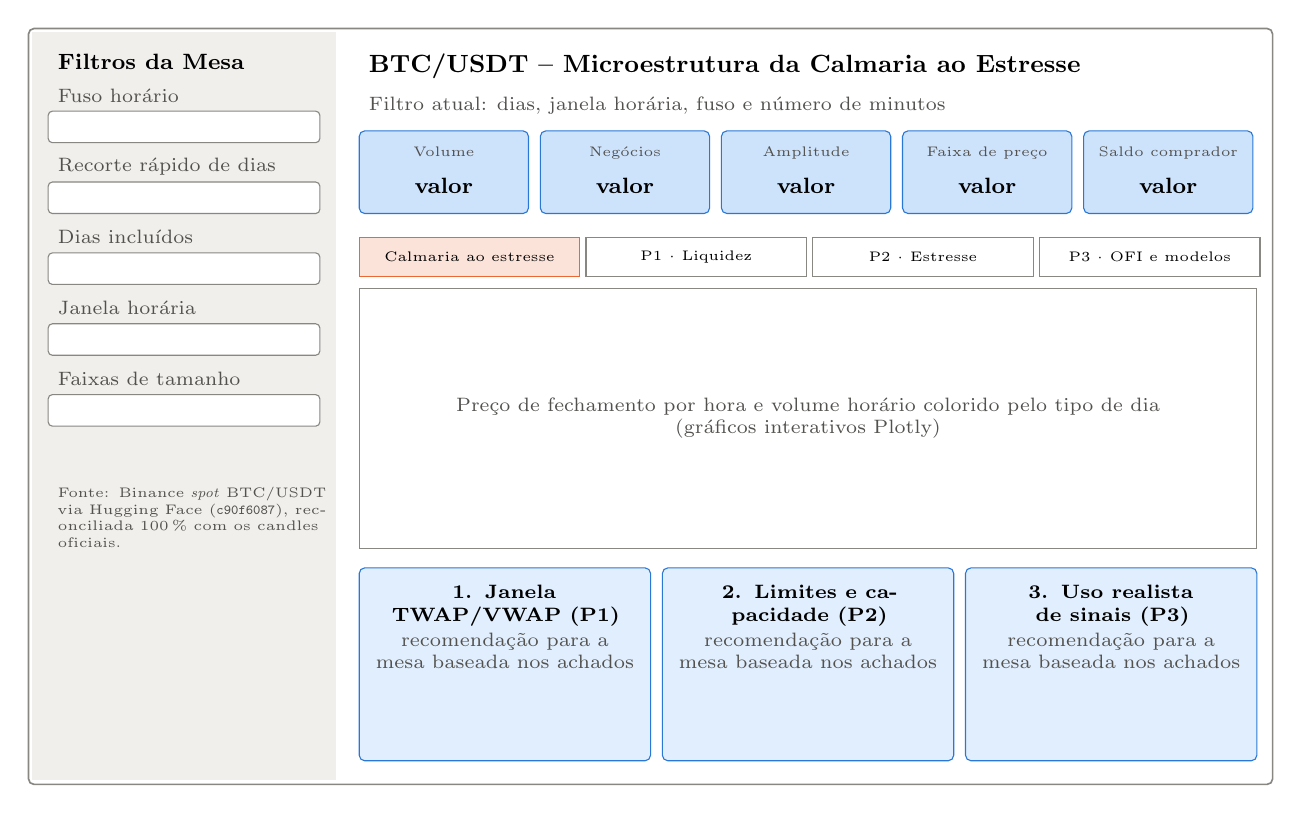
\begin{tikzpicture}[font=\scriptsize, x=1cm, y=1cm]
  % moldura
  \draw[cinza, line width=0.6pt, rounded corners=2pt] (0,0) rectangle (15.8,9.6);
  % barra lateral
  \fill[cinzaclaro] (0.05,0.05) rectangle (3.9,9.55);
  \node[anchor=north west, font=\footnotesize\bfseries] at (0.25,9.4) {Filtros da Mesa};
  \foreach \y/\t in {8.6/Fuso horário, 7.7/Recorte rápido de dias, 6.8/Dias incluídos, 5.9/Janela horária, 5.0/Faixas de tamanho}{
    \node[anchor=west, text=tinta] at (0.25,\y+0.15) {\t};
    \draw[cinza, fill=white, rounded corners=1.5pt] (0.25,\y-0.45) rectangle (3.7,\y-0.05);
  }
  \node[anchor=north west, text width=3.4cm, align=left, text=tinta, font=\tiny] at (0.25,3.9)
    {Fonte: Binance \textit{spot} BTC/USDT via Hugging Face (\texttt{c90f6087}), reconciliada 100\,\% com os candles oficiais.};
  % título e legenda
  \node[anchor=north west, font=\small\bfseries] at (4.2,9.4) {BTC/USDT -- Microestrutura da Calmaria ao Estresse};
  \node[anchor=north west, text=tinta] at (4.2,8.85) {Filtro atual: dias, janela horária, fuso e número de minutos};
  % KPIs
  \foreach \i/\t in {0/Volume, 1/Negócios, 2/Amplitude, 3/Faixa de preço, 4/Saldo comprador}{
    \pgfmathsetmacro{\x}{4.2+\i*2.3}
    \draw[azul, fill=azulclaro, rounded corners=2pt] (\x,7.25) rectangle (\x+2.15,8.3);
    \node[anchor=north, font=\tiny, text=tinta] at (\x+1.075,8.22) {\t};
    \node[font=\footnotesize\bfseries] at (\x+1.075,7.6) {valor};
  }
  % abas
  \foreach \i/\t in {0/Calmaria ao estresse, 1/P1 $\cdot$ Liquidez, 2/P2 $\cdot$ Estresse, 3/P3 $\cdot$ OFI e modelos}{
    \pgfmathsetmacro{\x}{4.2+\i*2.88}
    \ifnum\i=0
      \draw[laranja, fill=laranjaclaro] (\x,6.45) rectangle (\x+2.8,6.95);
    \else
      \draw[cinza, fill=white] (\x,6.45) rectangle (\x+2.8,6.95);
    \fi
    \node[font=\tiny] at (\x+1.4,6.7) {\t};
  }
  % conteúdo
  \draw[cinza, fill=white] (4.2,3.0) rectangle (15.6,6.3);
  \node[text=tinta, align=center] at (9.9,4.65) {Preço de fechamento por hora e volume horário colorido pelo tipo de dia\\(gráficos interativos Plotly)};
  \foreach \i/\t in {0/{1. Janela TWAP/VWAP (P1)}, 1/{2. Limites e capacidade (P2)}, 2/{3. Uso realista de sinais (P3)}}{
    \pgfmathsetmacro{\x}{4.2+\i*3.85}
    \draw[azul, fill=azulclaro!60, rounded corners=2pt] (\x,0.3) rectangle (\x+3.7,2.75);
    \node[anchor=north, text width=3.4cm, align=center, font=\scriptsize\bfseries] at (\x+1.85,2.65) {\t};
    \node[anchor=north, text width=3.4cm, align=center, text=tinta] at (\x+1.85,2.05) {recomendação para a mesa baseada nos achados};
  }
\end{tikzpicture}
\end{center}
\fonte{Elaborada pelos autores (2026). Esquema ilustrativo da disposição dos elementos de \texttt{app/dashboard.py}, não uma captura de tela.}
\end{figure}

\begin{quadro}[htbp]
\caption{\label{qua:abas}Indicadores e conteúdo das abas do painel}
\begin{corpotabela}
\begin{tabularx}{\textwidth}{|L{3.3cm}|Y|}
\hline
\textbf{Elemento} & \textbf{Conteúdo} \\ \hline
Indicadores do topo & Volume negociado (\usd~bilhões); negócios executados (milhões); amplitude mediana de 1 minuto (bps); faixa de preço (mínima a máxima); saldo comprador líquido (\% do volume) \\ \hline
Aba ``Da Calmaria ao Estresse'' & Preço de fechamento por hora e volume horário colorido pelo tipo de dia; plano de ação da mesa em três cartões: janela TWAP/VWAP (P1), limites e capacidade em estresse (P2) e uso realista de sinais preditivos (P3) \\ \hline
Aba ``P1 $\cdot$ Liquidez Intradiária'' & Medianas por hora de volume, negócios e amplitude, com as três horas de maior volume em destaque; mapa de calor de volume por dia e hora; dispersão entre volume e amplitude por hora, com o $\rho$ de Spearman no título \\ \hline
Aba ``P2 $\cdot$ Estresse \& Faixas de Tamanho'' & Volume e volatilidade realizada por dia, coloridos pelo tipo de dia; tabela de médias por regime; participação de cada faixa na contagem e no valor dos negócios; número de ordens agressoras de \usd~100 mil ou mais por dia \\ \hline
Aba ``P3 $\cdot$ Fluxo (OFI) \& Modelagem'' & Saldo líquido diário do fluxo agressor; correlação de Pearson entre $\mathrm{OFI}_t$ e $r_{t+k}$ para $k$ de 0 a 10, com a faixa de ruído de 95\,\%; tabelas-resumo da validação \textit{walk-forward} para volatilidade e direção \\ \hline
\end{tabularx}
\end{corpotabela}
\fonteautores[Elaborado]
\end{quadro}

\section{Execução}\label{sec:dashexecucao}

Com os Parquets gerados (\autoref{sec:comoexecutar}), o painel é iniciado a
partir da raiz do repositório com o comando abaixo e abre no navegador, por
padrão em \url{http://localhost:8501}.

\begin{lstlisting}[language=bash]
streamlit run app/dashboard.py
\end{lstlisting}

A primeira carga é a mais lenta, porque executa a validação
\textit{walk-forward} e grava o \textit{cache} de faixas de tamanho; as interações
seguintes reutilizam os resultados memorizados. O teste automatizado
\code{test_streamlit_dashboard_renders_without_errors} executa o painel sem
navegador e verifica que ele renderiza sem exceções, com cinco indicadores e
quatro abas.

% =============================================================================
\chapter{\textit{Data Storytelling}}\label{cap:storytelling}
% =============================================================================

A comunicação dos resultados foi pensada para quem decide na mesa de execução,
não para especialistas em estatística. Este capítulo descreve os princípios de
visualização adotados, a narrativa em três atos e a matriz de decisão que fecha o
projeto. A versão textual da narrativa está em \code{STORYTELLING.md}; a versão
visual, no notebook do \textit{Checkpoint}~3 e na primeira aba do painel.

\section{Princípios de visualização}\label{sec:principios}

Os gráficos seguem as recomendações de \citeonline{knaflic2018} de reduzir
elementos que não informam e direcionar a atenção para a mensagem. As regras
aplicadas em todos os gráficos do projeto foram:

\begin{alineas}
  \item \textbf{título-manchete}: o título principal de cada gráfico enuncia a
        conclusão (por exemplo, ``O fluxo explica o minuto em que acontece, mas
        quase nada do minuto seguinte''), e o subtítulo descreve o conteúdo;
  \item \textbf{cor com função fixa}: azul para compra ou série principal,
        laranja para venda ou alerta e tons de cinza para contexto, com paleta
        validada para daltonismo (protanopia, deuteranopia e tritanopia);
  \item \textbf{destaque seletivo}: apenas o que sustenta a conclusão recebe cor
        forte, como as três horas de maior volume na
        \autoref{fig:perfilhorario} ou o coeficiente do mesmo minuto na
        \autoref{fig:defasagens};
  \item \textbf{escalas honestas}: escala logarítmica para distribuições de
        cauda pesada, medianas quando a média distorce e faixa de ruído
        explícita nas correlações;
  \item \textbf{números no padrão brasileiro}: vírgula decimal, ponto como
        separador de milhar e horários em UTC com a conversão para BRT
        indicada.
\end{alineas}

\section{Narrativa em três atos}\label{sec:narrativa}

A narrativa ``Da calmaria ao estresse'' organiza os achados como uma história em
três atos, cada um ligado a uma pergunta de negócio e a uma decisão. A
\autoref{fig:storytelling} reúne as três evidências centrais em uma única
imagem, pensada para a apresentação executiva.

\begin{figure}[htbp]
\caption{\label{fig:storytelling}Síntese visual da narrativa ``Da calmaria ao estresse''}
\begin{center}
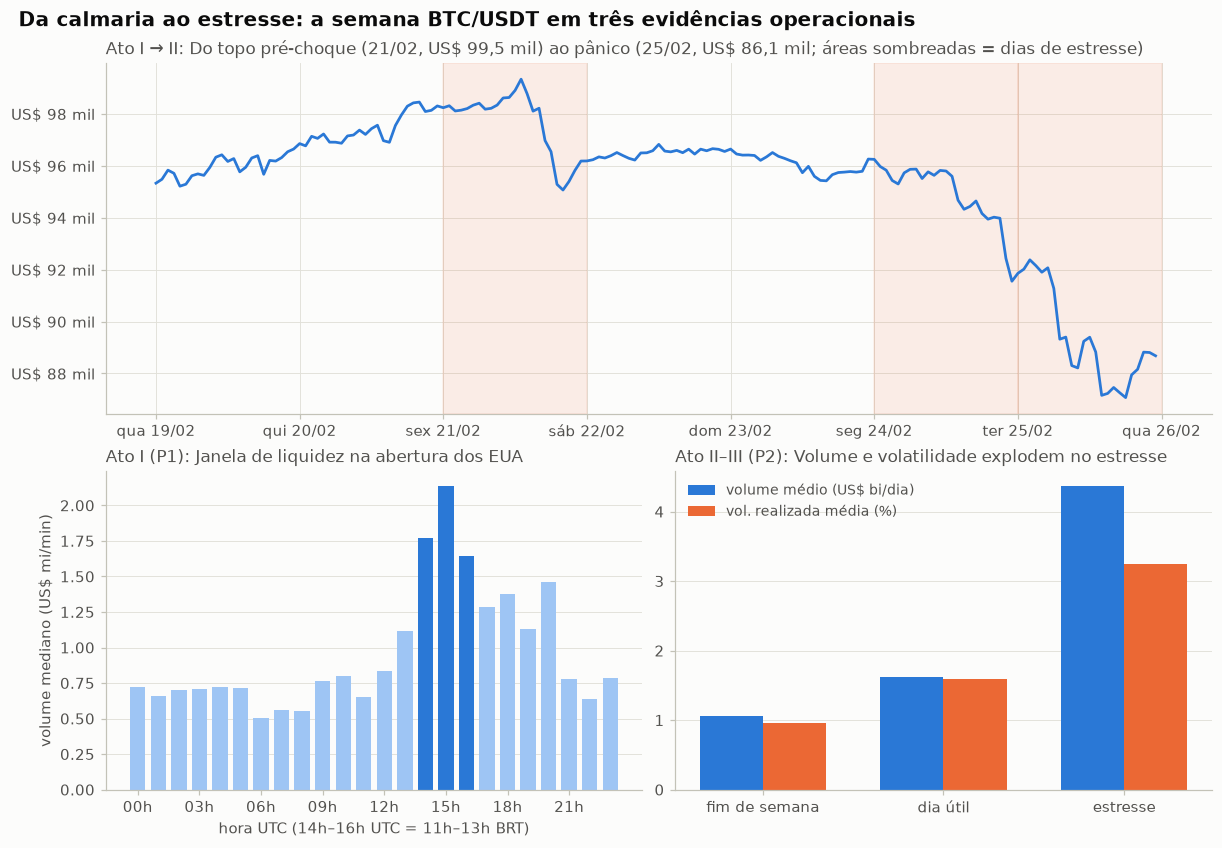
\includegraphics[width=\textwidth]{figuras/fig_storytelling.png}
\end{center}
\fontedados
\end{figure}

\textbf{Ato I -- O ritmo da calmaria (P1).} O mercado de BTC/USDT funciona
24 horas por dia, mas a liquidez não é uniforme: o volume mediano às 15h~UTC
(12h em Brasília) é 4,2 vezes o das 06h~UTC. O horário mais ativo coincide com a
abertura do mercado acionário americano. O dilema da mesa é que liquidez e
volatilidade caminham juntas ($\rho = 0,83$ entre as horas): entrar às 15h~UTC
reduz o impacto no livro, mas expõe uma ordem única a oscilações maiores.
\textbf{Decisão}: executar ordens institucionais dentro da janela líquida, sempre
fatiadas por TWAP ou VWAP.

\textbf{Ato II -- O choque e a escalada ao pânico (P2).} Na sexta-feira, 21/02, o
ataque à Bybit desencadeou uma mudança abrupta de regime. O bitcoin caiu 13,5\,\%
em quatro dias, com saldo vendedor em todos os dias da semana. Nos dias de
estresse, o volume foi 2,7 vezes e a volatilidade 2,0 vezes a de um dia útil; em
25/02 ocorreram 10,3 milhões de negócios e quase 10 mil ordens agressoras de
\usd~100 mil ou mais. Movimentos além de $3\sigma$ foram 6,9 vezes mais
frequentes que o previsto pela curva normal. \textbf{Decisão}: abandonar limites
estáticos e dimensionar a infraestrutura para picos de 4 a 5 vezes a carga
normal.

\textbf{Ato III -- Fluxo, modelos e os limites da eficiência (P3).} O fluxo
agressor empurra o preço no instante da execução (correlação de 0,388 no mesmo
minuto), mas quase não antecipa o minuto seguinte (0,022). Nenhum modelo
direcional, em 1 minuto ou 1 segundo, gerou ganho bruto capaz de pagar as taxas.
Em contrapartida, a volatilidade do próximo minuto é previsível fora da amostra
($R^2 = 0,385$). \textbf{Decisão}: usar a previsão de volatilidade para calibrar
limites e ritmo de execução, e não usar o OFI para operar direção.

\section{Matriz de decisão}\label{sec:matriz}

O \autoref{qua:matriz} consolida as recomendações em formato de matriz de
decisão, que é o fechamento da narrativa e o principal entregável para o
público executivo.

\begin{quadro}[htbp]
\caption{\label{qua:matriz}Matriz de decisão para a mesa de execução}
\begin{corpotabela}
\begin{tabularx}{\textwidth}{|L{2.7cm}|Y|L{5.4cm}|}
\hline
\textbf{Alavanca da mesa} & \textbf{Evidência empírica} & \textbf{Ação recomendada} \\ \hline
Janela de execução (TWAP/VWAP) & Pico às 15h~UTC com \usd~2,13 mi/min contra \usd~0,51 mi/min às 06h~UTC (4,2 vezes); Spearman entre volume e amplitude de 0,83 & Programar execuções grandes preferencialmente entre 14h e 16h~UTC (11h e 13h~BRT), sempre fatiadas; em dias de choque, monitorar deslocamentos da liquidez, como o pico às 07h~UTC de 25/02 \\ \hline
Limites de risco e \textit{slippage} & Em estresse, volatilidade realizada 2,0 vezes maior; 1,87\,\% dos minutos além de $3\sigma$ (6,9 vezes a normal); volatilidade de $t+1$ previsível ($R^2 = 0,385$; Spearman de 0,616) & Calibrar limites de \textit{slippage} e de perda dinamicamente pela volatilidade prevista pelo Ridge e pela realizada em janela móvel, abandonando bandas fixas baseadas na curva normal \\ \hline
Capacidade operacional & 25/02 teve 10,3 milhões de negócios (37\,\% da semana) e quase 10 mil ordens de \usd~100 mil ou mais (4,5 vezes um dia útil) & Dimensionar ingestão e roteamento para pelo menos 4 a 5 vezes o volume de negócios de um dia útil, sem perda de latência \\ \hline
Uso de sinais de fluxo (OFI) & Correlação de 0,388 no mesmo minuto e de 0,022 no minuto seguinte; ganho bruto direcional abaixo de 0,4~bps contra custos de 2 a 10~bps por perna & Não operar estratégia direcional com base no OFI; usá-lo apenas como filtro auxiliar para evitar cruzar o \textit{spread} contra um fluxo extremo imediato \\ \hline
\end{tabularx}
\end{corpotabela}
\fonteautores[Elaborado]
\end{quadro}

Os \textit{slides} da defesa final, último entregável pendente do
\textit{Checkpoint}~3, devem seguir esta mesma estrutura: problema, três atos e
matriz de decisão, reaproveitando as figuras deste documento.

% =============================================================================
\chapter{Ética, LGPD e limitações}\label{cap:etica}
% =============================================================================

Este capítulo consolida a análise de governança do projeto: a conformidade com a
LGPD \cite{brasil2018}, o respeito à licença da fonte, os vieses e limitações dos
dados e do método e os riscos de transformar análises estatísticas em decisões
automatizadas. A versão detalhada está em \code{ETHICS_LGPD.md}.

\section{Conformidade com a LGPD}\label{sec:lgpd}

Nos termos do art.~5º, inciso~I, da LGPD, dado pessoal é a ``informação
relacionada a pessoa natural identificada ou identificável''
\cite[art.~5º, I]{brasil2018}. A base analisada contém exclusivamente registros
públicos de execução no livro de ofertas à vista de BTC/USDT da Binance. O
\autoref{qua:lgpd} avalia cada campo.

\begin{quadro}[htbp]
\caption{\label{qua:lgpd}Avaliação dos campos da base quanto à presença de dados pessoais}
\begin{corpotabela}
\begin{tabularx}{\textwidth}{|L{3.0cm}|Y|L{4.6cm}|}
\hline
\textbf{Campo} & \textbf{Natureza} & \textbf{Contém dado pessoal?} \\ \hline
\code{trade_id} & Número sequencial atribuído pelo motor de casamento da corretora & Não. Identifica um evento de mercado, sem vínculo público com conta, CPF, CNPJ ou carteira \\ \hline
\code{exchange_ts} (\code{ts}) & Instante da execução pública, em UTC & Não. Metadado temporal de mercado \\ \hline
\code{price}, \code{quantity} & Preço e quantidade executados no livro público & Não. Informação pública de formação de preço \\ \hline
\code{aggressor_side} (\code{side}) & Lado do agressor (compra ou venda) & Não. Dinâmica impessoal de oferta e demanda \\ \hline
\code{exchange}, \code{symbol} & Constantes técnicas (\code{binance}, \code{BTCUSDT}) & Não \\ \hline
\code{ingest_ts} & Carimbo de coleta do fornecedor, 100\,\% inválido & Não; além disso, foi descartado na limpeza \\ \hline
\end{tabularx}
\end{corpotabela}
\fonteautores[Elaborado]
\end{quadro}

Não há titular identificável nem dado pessoal sensível (art.~5º, II). Como a LGPD
regula o tratamento de dados pessoais, o tratamento de dados de mercado anônimos
fica fora do seu escopo. Mesmo que houvesse dado pessoal, o art.~4º, inciso~II,
alínea~b, afasta a aplicação da lei ao tratamento realizado para fins
exclusivamente acadêmicos, ressalvados os arts.~7º e 11.

Ainda assim, o projeto aplica, por boa prática, os princípios do art.~6º. Pelo
princípio da \textbf{necessidade}, foram removidas as colunas constantes,
redundantes e corrompidas, mantendo-se apenas o necessário às perguntas de
negócio. Pelo princípio da \textbf{qualidade dos dados}, a base passou por
contrato de qualidade e por validação cruzada com a fonte primária. Pelo
princípio da \textbf{transparência}, todas as decisões de tratamento estão
documentadas.

\section{Risco residual de reidentificação}\label{sec:reidentificacao}

Embora a base isolada seja impessoal, em uma mesa real existiria um risco
conceitual de reidentificação indireta se os registros públicos fossem cruzados
com logs internos de ordens da própria mesa, com cadastros de clientes
(processos de identificação de clientes, ou KYC) ou com movimentações em
\textit{blockchain} próximas ao instante de uma ordem. O projeto mitiga esse risco
de três formas: opera exclusivamente sobre o fluxo público, sem nenhum
cruzamento com cadastros, carteiras ou logs de clientes; trabalha
predominantemente com agregações temporais (barras de 1 minuto e 1 segundo); e
reconstrói ordens agressoras apenas por contiguidade temporal, sem atribuição de
autoria.

\section{Licença e reprodutibilidade}\label{sec:licenca}

A base está sob licença de uso pessoal e acadêmico, com redistribuição proibida
\cite{glitchlist2026}. Os controles técnicos adotados são:

\begin{alineas}
  \item \textbf{sem redistribuição}: o arquivo \code{.gitignore} bloqueia toda a
        pasta \code{data/}; nenhum Parquet bruto ou processado é versionado;
  \item \textbf{download na origem e imutabilidade}: o código fixa o
        \textit{commit} da base no Hugging Face e confere o SHA-256 antes de
        qualquer processamento;
  \item \textbf{finalidade acadêmica}: código, documentação e painel destinam-se
        à avaliação da unidade curricular e à demonstração metodológica em um
        cenário simulado;
  \item \textbf{fonte primária apenas para validação}: os candles da Binance
        \cite{binance2025} são usados somente para reconciliar a base.
\end{alineas}

As figuras deste documento mostram apenas agregações e estatísticas derivadas,
não os registros da base.

\section{Vieses e limitações}\label{sec:vieses}

O recorte escolhido traz vieses que limitam a generalização dos resultados. O
\autoref{qua:vieses} resume cada um e o seu impacto na interpretação.

\begin{quadro}[htbp]
\caption{\label{qua:vieses}Vieses e limitações dos dados e do método}
\begin{corpotabela}
\begin{tabularx}{\textwidth}{|L{3.3cm}|Y|L{5.0cm}|}
\hline
\textbf{Dimensão} & \textbf{Limitação} & \textbf{Impacto na interpretação} \\ \hline
Seleção temporal & Apenas 7 dias (19 a 25/02/2025), marcados pelo ataque à Bybit e por queda de 13,5\,\%; saldo vendedor em todos os dias & Os padrões não representam semanas neutras ou de alta \\ \hline
Única corretora & Somente a Binance \textit{spot}, a de maior liquidez global & Outras corretoras e mercados de derivativos podem ter horários de pico e profundidade diferentes \\ \hline
Único par & Somente BTC/USDT, o par mais líquido do mercado & Outros criptoativos e pares contra moeda fiduciária têm \textit{spreads} e lacunas de liquidez maiores \\ \hline
Amostra horária curta & Apenas 7 observações por hora do dia, das quais 3 em estresse & As medianas horárias são indicativas, não definitivas \\ \hline
Reconstrução de ordens & Negócios do mesmo milissegundo e lado são fundidos em uma ordem & Ordens independentes simultâneas podem ser somadas \\ \hline
Qualidade do fornecedor & \code{ingest_ts} 100\,\% inválido e período declarado incorreto & Impede qualquer análise de latência de coleta; exigiu validação cruzada integral \\ \hline
Sem livro de ofertas & A base contém apenas negócios, sem cotações nem profundidade & Não é possível medir o \textit{spread} cotado ou a liquidez em repouso, apenas o impacto realizado \\ \hline
\end{tabularx}
\end{corpotabela}
\fonteautores[Elaborado]
\end{quadro}

\section{Riscos do uso de sinais de mercado}\label{sec:riscos}

Mesmo com uma base limpa e validada, transformar análises em decisões
automatizadas envolve riscos que a mesa precisa conhecer:

\begin{alineas}
  \item \textbf{ilusão preditiva diante dos custos}: acurácia ou ROC-AUC acima de
        50\,\% não implica lucro; o ganho bruto dos sinais direcionais é muito menor
        que as taxas, e operá-los geraria prejuízo por excesso de giro;
  \item \textbf{quebra de regime}: modelos treinados em dias calmos subestimam a
        escala da volatilidade e o tamanho das ordens durante choques; a
        reavaliação contínua em janelas \textit{walk-forward} e limites rígidos
        baseados em volatilidade são indispensáveis;
  \item \textbf{vazamento de futuro e mineração de dados}: interpolação de lacunas,
        normalização antes da divisão entre treino e teste ou atributos com
        \code{shift(-1)} criam acurácia artificial; o projeto evita esses erros e os
        testa automaticamente;
  \item \textbf{impacto próprio e retroalimentação}: uma mesa que executa ordens
        grandes sempre no mesmo horário, ou que reage mecanicamente ao OFI, passa
        a gerar ela própria o desequilíbrio observado e aumenta o próprio
        \textit{slippage};
  \item \textbf{uso responsável}: os modelos são recomendados exclusivamente como
        \textbf{apoio à decisão}, com supervisão humana, para dimensionar janelas
        de execução e calibrar limites, e não como motor autônomo de
        negociação.
\end{alineas}

% =============================================================================
\chapter{Testes e reprodutibilidade}\label{cap:reprodutibilidade}
% =============================================================================

\section{Testes automatizados}\label{sec:testes}

O arquivo \code{tests/test_etl_and_modeling.py} reúne sete testes escritos com
pytest. Seis deles usam pequenos conjuntos sintéticos e não dependem da base
real; o sétimo executa o painel e só roda quando os Parquets processados estão
disponíveis (\autoref{qua:testes}).

\begin{quadro}[htbp]
\caption{\label{qua:testes}Testes automatizados do projeto}
\begin{corpotabela}
\begin{tabularx}{\textwidth}{|L{6.4cm}|Y|}
\hline
\textbf{Teste} & \textbf{O que garante} \\ \hline
\code{test_clean_and_validate_trades_contract} & A limpeza remove \code{ingest_ts} inválido e as colunas constantes, preserva \code{exchange} e \code{symbol} nos metadados, mapeia corretamente o lado do agressor e produz uma base que passa no contrato de qualidade \\ \hline
\code{test_build_bars_and_fill_bar_gaps_no_lookahead} & A grade de 1 segundo tem o número correto de barras; segundos vazios aparecem como nulos e são preenchidos com o preço \textbf{anterior}, nunca com o futuro; volume zero, OFI neutro e VWAP igual ao último preço \\ \hline
\code{test_build_taker_orders_merges_consecutive_same_ts_and_side} & Negócios consecutivos de mesmo milissegundo e lado formam uma única ordem, com quantidade somada e \textit{book walk} positivo \\ \hline
\code{test_build_lagged_features_strictly_causal_no_lookahead} & Perturbar drasticamente preços, OFI e volume a partir de um instante não altera nenhum atributo anterior a ele \\ \hline
\code{test_daily_walk_forward_folds_chronological} & Todas as observações de treino são anteriores ao dia de teste, e cada dobra testa exatamente um dia \\ \hline
\code{test_prepare_modeling_dataset_shapes} & O conjunto de modelagem não tem nulos, atributos e alvos têm o mesmo tamanho, e os grupos de atributos existem nas colunas \\ \hline
\code{test_streamlit_dashboard_renders_without_errors} & O painel renderiza sem exceções, com cinco indicadores e quatro abas (ignorado se os Parquets não existirem) \\ \hline
\end{tabularx}
\end{corpotabela}
\fonteautores[Elaborado]
\end{quadro}

Para esta documentação, a suíte foi executada em 25/11/2026, em ambiente limpo,
com Python 3.13, pandas 3.0, NumPy 2.5, scikit-learn 1.9 e Streamlit 1.67. O
resultado foi de \textbf{seis testes aprovados e um ignorado}: o teste do painel
foi ignorado porque, nesse ambiente, os Parquets processados não haviam sido
gerados.

\section{Como executar}\label{sec:comoexecutar}

\subsection{No Google Colab}\label{sec:colab}

É a forma recomendada para o notebook do \textit{Checkpoint}~2, que baixa os
dados sozinho: no Colab, escolher \textit{Arquivo} $\rightarrow$ \textit{Fazer
upload de notebook}, selecionar o arquivo \code{.ipynb} e então
\textit{Ambiente de execução} $\rightarrow$ \textit{Executar tudo}. A execução
leva de 1 a 3 minutos e cabe na memória do Colab gratuito.

\subsection{Localmente}\label{sec:local}

A partir da raiz do repositório, criar um ambiente virtual e instalar as
dependências:

\begin{lstlisting}[language=bash]
python -m venv .venv && source .venv/bin/activate
pip install -r requirements.txt
\end{lstlisting}

Em seguida, gerar e validar os Parquets de \code{data/processed/} pelo pipeline
consolidado (a função é idempotente: se os arquivos já existirem, nada é
refeito):

\begin{lstlisting}[language=bash]
python -m src.etl
\end{lstlisting}

Os notebooks são abertos a partir da pasta \code{notebooks/}, o painel é iniciado
como descrito na \autoref{sec:dashexecucao}, e os testes rodam a partir da raiz:

\begin{lstlisting}[language=bash]
cd notebooks && jupyter notebook A3_CP3_modelagem_storytelling.ipynb
streamlit run app/dashboard.py
python -m pytest -q tests/
\end{lstlisting}

\section{Requisitos de ambiente e cuidados com memória}\label{sec:memoria}

A base tem 27,9 milhões de linhas, e o Colab gratuito oferece cerca de 12~GB de
RAM. O pico de uso medido foi de aproximadamente 6~GB com pandas~3 e 9~GB com
pandas~2.2. Para caber nesse limite, o projeto adota as seguintes técnicas:

\begin{alineas}
  \item textos armazenados no formato compacto do Arrow (padrão no pandas 3 e
        ativado explicitamente no 2.x);
  \item alocador de memória do sistema no PyArrow, que devolve ao sistema
        operacional a memória liberada, e liberação explícita após leituras
        grandes;
  \item transformação sobre o próprio \textit{DataFrame} carregado, com o bruto
        preservado em disco, e remoção de objetos auxiliares seguida de coleta de
        lixo;
  \item leitura apenas das colunas necessárias nos produtos derivados e
        \textit{cache} das agregações usadas pelo painel.
\end{alineas}

A correlação de Spearman no pandas depende da biblioteca SciPy, que não aparece
explicitamente em \code{requirements.txt}, mas é instalada como dependência do
scikit-learn e já vem no Colab.

\section{Garantias de reprodutibilidade}\label{sec:garantias}

Os resultados podem ser reproduzidos por qualquer pessoa porque o projeto fixa
todas as fontes de variação controláveis:

\begin{alineas}
  \item \textbf{dados}: \textit{commit} da base e SHA-256 fixados; candles da
        Binance conferidos pelo SHA-256 publicado pela própria corretora;
  \item \textbf{código}: um único pacote (\code{src/}) compartilhado por
        notebooks, painel e testes, versionado em Git;
  \item \textbf{aleatoriedade}: semente fixa (\code{random_state=42}) nos modelos
        de árvore; os demais modelos são determinísticos;
  \item \textbf{ordem temporal}: dobras \textit{walk-forward} cronológicas e
        atributos estritamente causais, verificados por testes.
\end{alineas}

% =============================================================================
\chapter{Considerações finais}\label{cap:consideracoes}
% =============================================================================

O Projeto Analítico A3 transformou uma base pública de 27,9 milhões de negócios
de BTC/USDT em evidências para as decisões de uma mesa de execução de
criptoativos, cobrindo todas as etapas previstas nas diretrizes da disciplina:
diagnóstico, ETL com auditoria de qualidade, análise exploratória, modelagem
preditiva, visualização e reflexão ética.

A primeira contribuição do trabalho está na qualidade dos dados. Uma base que
parecia limpa, sem nenhum nulo, escondia um carimbo de ingestão 100\,\% inválido
e 41,7\,\% de duplicatas aparentes que, se removidas por um procedimento
ingênuo, teriam destruído quase metade dos negócios. A reconciliação minuto a
minuto com a fonte oficial, com concordância total nos 10.080 minutos, deu
segurança para todas as análises seguintes e é a melhor ilustração do princípio
\textit{Garbage In, Garbage Out} no projeto.

As três perguntas de negócio foram respondidas com números. Na P1, a liquidez se
concentra entre 14h e 16h~UTC, com pico 4,2 vezes maior que o vale, mas acompanhada
de volatilidade mais alta, o que recomenda execução fatiada nessa janela. Na P2,
os dias de estresse multiplicam o volume por 2,7 e a volatilidade por 2,0, e o
valor negociado é dominado por poucos negócios grandes, o que exige limites de
risco dinâmicos e folga de capacidade. Na P3, o desequilíbrio do fluxo explica o
preço do mesmo minuto, mas não o do minuto seguinte.

A modelagem preditiva confirmou e refinou essas conclusões. A volatilidade do
intervalo seguinte é previsível fora da amostra, e a regressão Ridge superou
tanto os \textit{baselines} quanto os modelos de árvore. A direção do preço, por
outro lado, não oferece ganho que cubra os custos de transação, nem mesmo na
escala de 1 segundo, em que a alta acurácia apenas reflete o \textit{bid-ask
bounce}. Para a mesa, o valor prático está na gestão de risco e no ritmo de
execução, e não em apostas direcionais.

As conclusões devem ser lidas à luz das limitações discutidas no
\autoref{cap:etica}: uma única semana, atípica, de uma única corretora e de um
único par. Como trabalhos futuros, recomenda-se:

\begin{alineas}
  \item repetir as análises em mais semanas, incluindo períodos calmos e de alta,
        e em outras corretoras e pares, para validar a estabilidade dos padrões
        horários e de estresse;
  \item incorporar dados do livro de ofertas, para medir o \textit{spread}
        cotado, a profundidade e o OFI na forma original de
        \citeonline{cont2014};
  \item comparar a previsão de volatilidade com modelos econométricos clássicos
        de volatilidade realizada e avaliar seu uso em uma simulação de execução
        TWAP e VWAP com custos;
  \item evoluir o pipeline para processamento contínuo, com o mesmo contrato de
        qualidade aplicado a cada novo lote de dados.
\end{alineas}

No momento desta documentação, as pendências do projeto, registradas em
\code{TODO.md}, são a elaboração dos \textit{slides} da defesa final, a
atualização da tabela de entregas no \code{README.md} e uma revisão de
reprodutibilidade de ponta a ponta dos notebooks, do código consolidado e do
painel antes da entrega.


% ---------------------------------------------------------------------------------
% ELEMENTOS PÓS-TEXTUAIS
% ---------------------------------------------------------------------------------
\postextual

\bibliography{referencias}

\begin{apendicesenv}
% =============================================================================
\chapter{Matriz de atendimento aos requisitos e à rubrica da A3}\label{apendice:matriz}
% =============================================================================

O \autoref{qua:rubrica} relaciona cada critério da rubrica de avaliação da A3
\cite{usjt2026} às seções deste documento e aos arquivos do repositório que o
atendem. O \autoref{qua:regras} faz o mesmo com as regras gerais do projeto.

\begin{quadro}[htbp]
\caption{\label{qua:rubrica}Critérios da rubrica da A3 e onde são atendidos}
\begin{corpotabela}
\begin{tabularx}{\textwidth}{|L{3.4cm}|C{1.2cm}|Y|L{3.8cm}|}
\hline
\textbf{Critério} & \textbf{Pontos} & \textbf{Onde é atendido neste documento} & \textbf{Arquivos do repositório} \\ \hline
1. Diagnóstico do problema e \textit{dataset} & 5,0 & Contexto, objetivos e perguntas (\autoref{cap:introducao}); base, aderência e dicionário (\autoref{cap:base}) & \code{CHECKPOINT_1.md} \\ \hline
2. Qualidade do código e processo ETL & 10,0 & Arquitetura e módulos (\autoref{cap:arquitetura}); auditoria, nulos, duplicatas, tipos, contrato e validação cruzada (\autoref{cap:etl}); testes (\autoref{cap:reprodutibilidade}) & Notebook do CP2; \code{src/etl.py}; \code{tests/} \\ \hline
3. Análise exploratória e métricas & 10,0 & Estatísticas, \code{groupby}, séries temporais, correlações e respostas P1 a P3 (\autoref{cap:eda}); modelagem (\autoref{cap:modelagem}) & Notebooks do CP2 e do CP3; \code{src/data_loader.py}; \code{src/modeling.py} \\ \hline
4. \textit{Data Storytelling} e visualização & 10,0 & Gráficos (\autoref{cap:eda} e \autoref{cap:modelagem}); painel (\autoref{cap:dashboard}); narrativa e matriz de decisão (\autoref{cap:storytelling}) & \code{app/dashboard.py}; \code{STORYTELLING.md}; notebook do CP3 \\ \hline
5. Ética, LGPD e comunicação & 5,0 & LGPD, reidentificação, licença, vieses e riscos (\autoref{cap:etica}) & \code{ETHICS_LGPD.md}; \textit{slides} (pendentes) \\ \hline
\end{tabularx}
\end{corpotabela}
\fonteautores[Elaborado]
\end{quadro}

\begin{quadro}[htbp]
\caption{\label{qua:regras}Regras gerais da A3 e situação do projeto}
\begin{corpotabela}
\begin{tabularx}{\textwidth}{|L{4.6cm}|Y|C{2.0cm}|}
\hline
\textbf{Regra} & \textbf{Evidência} & \textbf{Situação} \\ \hline
Grupo de 2 a 3 alunos & 2 integrantes (\autoref{sec:equipe}) & atendida \\ \hline
Base real e pública & Hugging Face, validada contra a Binance (\autoref{sec:fonte}) & atendida \\ \hline
Mínimo de 1.000 registros & 27.925.338 registros & atendida \\ \hline
De 8 a 10 colunas de tipos variados & 9 colunas numéricas, categóricas e temporais (\autoref{sec:dicionario}) & atendida \\ \hline
Oportunidades reais de limpeza & 14 achados registrados no log de auditoria (\autoref{sec:sinteseauditoria}) & atendida \\ \hline
CP1: grupo, cenário, base, dicionário e 3 perguntas & \code{CHECKPOINT_1.md} & entregue \\ \hline
CP2: notebook comentado com auditoria, tratamento, limpeza e EDA & \code{notebooks/A3_CP2_auditoria_etl_eda.ipynb} & entregue \\ \hline
CP3: \textit{slides}, painel ou gráficos, ética e LGPD, código consolidado & Painel, código, ética e esta documentação; \textit{slides} pendentes & parcial \\ \hline
\end{tabularx}
\end{corpotabela}
\fonteautores[Elaborado]
\end{quadro}

% =============================================================================
\chapter{Dicionário dos produtos analíticos}\label{apendice:dicionario}
% =============================================================================

Este apêndice descreve as colunas dos quatro arquivos Parquet gravados em
\code{data/processed/}. As barras de 1 minuto e de 1 segundo têm o mesmo
esquema, exceto pela coluna \code{has_trades}, exclusiva das barras de 1 segundo.

\begin{quadro}[htbp]
\caption{\label{qua:dictrades}Colunas de \texttt{trades\_clean.parquet} (1 linha por negócio)}
\begin{corpotabela}
\begin{tabularx}{\textwidth}{|L{2.8cm}|L{3.0cm}|Y|}
\hline
\textbf{Coluna} & \textbf{Tipo} & \textbf{Descrição} \\ \hline
\code{trade_id} & inteiro de 64 bits & Identificador sequencial do negócio na Binance (único e contíguo) \\ \hline
\code{ts} & data-hora UTC & Instante da execução, com precisão de milissegundo \\ \hline
\code{price} & real & Preço de execução (USDT por BTC) \\ \hline
\code{quantity} & real & Quantidade negociada (BTC) \\ \hline
\code{side} & categórica & Lado do agressor: \code{buy}, o comprador tomou a oferta; \code{sell}, o vendedor atingiu a demanda \\ \hline
\code{notional_usd} & real & Valor financeiro do negócio, \code{price} $\times$ \code{quantity} (\usd) \\ \hline
\code{size_bucket} & categórica ordenada & Faixa de valor do negócio \\ \hline
\end{tabularx}
\end{corpotabela}
\fonteautores[Elaborado]
\end{quadro}

\begin{quadro}[htbp]
\caption{\label{qua:dicbars}Colunas de \texttt{bars\_1min.parquet} e \texttt{bars\_1s.parquet} (1 linha por intervalo, índice \texttt{ts})}
\begin{corpotabela}
\begin{tabularx}{\textwidth}{|L{3.0cm}|L{2.0cm}|Y|}
\hline
\textbf{Coluna} & \textbf{Tipo} & \textbf{Descrição} \\ \hline
\code{open}, \code{high}, \code{low}, \code{close} & real & Primeiro, máximo, mínimo e último preço do intervalo (USDT) \\ \hline
\code{volume_btc} & real & Quantidade total negociada (BTC) \\ \hline
\code{volume_usd} & real & Valor total negociado (\usd) \\ \hline
\code{n_trades} & inteiro & Número de negócios \\ \hline
\code{buy_volume_btc} & real & Volume em que o agressor foi comprador (BTC) \\ \hline
\code{sell_volume_btc} & real & Volume em que o agressor foi vendedor (BTC) \\ \hline
\code{vwap} & real & Preço médio ponderado pelo volume; igual ao fechamento quando não há negócio \\ \hline
\code{ofi} & real & Desequilíbrio do fluxo agressor, entre $-1$ e $+1$ (\autoref{eq:ofi}); 0 quando não há negócio \\ \hline
\code{log_return} & real & Retorno logarítmico em relação ao fechamento anterior (\autoref{eq:retorno}) \\ \hline
\code{abs_return_bps} & real & Valor absoluto do retorno, em pontos-base \\ \hline
\code{range_bps} & real & Amplitude do intervalo, em pontos-base (\autoref{eq:amplitude}) \\ \hline
\code{avg_trade_usd} & real & Valor médio por negócio (\usd); 0 quando não há negócio \\ \hline
\code{has_trades} & booleano & Somente em 1~s: indica se houve negócio no segundo \\ \hline
\end{tabularx}
\end{corpotabela}
\fonteautores[Elaborado]
\end{quadro}

\begin{quadro}[htbp]
\caption{\label{qua:dicorders}Colunas de \texttt{taker\_orders.parquet} (1 linha por ordem agressora, índice \texttt{order\_id})}
\begin{corpotabela}
\begin{tabularx}{\textwidth}{|L{3.0cm}|L{2.4cm}|Y|}
\hline
\textbf{Coluna} & \textbf{Tipo} & \textbf{Descrição} \\ \hline
\code{ts} & data-hora UTC & Instante da primeira execução da ordem \\ \hline
\code{side} & categórica & Lado do agressor \\ \hline
\code{first_trade_id} & inteiro & Identificador do primeiro negócio da ordem \\ \hline
\code{n_fills} & inteiro & Número de execuções parciais agrupadas \\ \hline
\code{quantity} & real & Quantidade total da ordem (BTC) \\ \hline
\code{notional_usd} & real & Valor total da ordem (\usd) \\ \hline
\code{price_first}, \code{price_last} & real & Preço da primeira e da última execução \\ \hline
\code{book_walk_bps} & real & Distância entre o primeiro e o último preço executado, em pontos-base \\ \hline
\code{size_bucket} & categórica ordenada & Faixa de valor da ordem \\ \hline
\end{tabularx}
\end{corpotabela}
\fonteautores[Elaborado]
\end{quadro}

% =============================================================================
\chapter{Lista completa de atributos dos modelos}\label{apendice:atributos}
% =============================================================================

O \autoref{qua:listaatributos} lista os nomes das colunas geradas por
\code{build_lagged_features()}. Os sufixos \code{t0} e \code{lagN} indicam o
intervalo atual e a defasagem de $N$ intervalos; \code{ma_W} e \code{std_W}
indicam média e desvio-padrão móveis nos últimos $W$ intervalos.

\begin{quadro}[htbp]
\caption{\label{qua:listaatributos}Atributos de entrada dos modelos, por família}
\begin{corpotabela}
\begin{tabularx}{\textwidth}{|L{3.0cm}|Y|C{1.2cm}|}
\hline
\textbf{Família} & \textbf{Atributos} & \textbf{Total} \\ \hline
Fluxo (OFI) & \code{ofi_t0}, \code{ofi_lag1}, \code{ofi_lag2}, \code{ofi_lag3}, \code{ofi_lag5}, \code{ofi_ma_5}, \code{ofi_ma_15}, \code{ofi_ma_60} & 8 \\ \hline
Atividade & \code{log_vol_usd_t0}, \code{log_vol_usd_lag1}, \code{log_vol_usd_lag2}, \code{log_vol_usd_lag3}, \code{log_vol_usd_lag5}, \code{log_n_trades_t0}, \code{log_n_trades_lag1}, \code{log_n_trades_lag2}, \code{log_n_trades_lag3}, \code{log_n_trades_lag5}, \code{log_avg_trade_t0}, \code{log_vol_ma_5}, \code{log_vol_ma_15}, \code{log_vol_ma_60}, \code{ofi_x_log_vol_t0}; em 1~s, também \code{has_trades_t0} & 15 (16) \\ \hline
Volatilidade e retorno & \code{range_bps_t0}, \code{range_bps_lag1}, \code{range_bps_lag2}, \code{range_bps_lag3}, \code{range_bps_lag5}, \code{abs_ret_bps_t0}, \code{abs_ret_bps_lag1}, \code{abs_ret_bps_lag2}, \code{abs_ret_bps_lag3}, \code{abs_ret_bps_lag5}, \code{ret_bps_t0}, \code{ret_bps_lag1}, \code{ret_bps_lag2}, \code{ret_bps_lag3}, \code{ret_bps_lag5}, \code{range_bps_ma_5}, \code{range_bps_ma_15}, \code{range_bps_ma_60}, \code{abs_ret_bps_ma_5}, \code{abs_ret_bps_ma_15}, \code{abs_ret_bps_ma_60}, \code{ret_bps_std_5}, \code{ret_bps_std_15}, \code{ret_bps_std_60}, \code{range_ratio_5_60} & 25 \\ \hline
Sazonalidade & \code{sin_hour}, \code{cos_hour} & 2 \\ \hline
\multicolumn{2}{|r|}{\textbf{Total do conjunto \code{completo}}} & \textbf{50 (51)} \\ \hline
\end{tabularx}
\end{corpotabela}
\fonteautores[Elaborado]
\end{quadro}

\end{apendicesenv}

\end{document}
